\documentclass{template}
\usepackage{graphicx,subfig,parskip,appendix,float,geometry,titlesec,uarial,glossaries}

\geometry{
 a4paper,
 total={150mm,240mm},
 left=35mm,
 top=25mm,
 }

\usepackage[
    style=authoryear,
    natbib=true,
    doi=true,
    giveninits=true
]{biblatex}

\DeclareFieldFormat{url}{%
    \mkbibacro{Available at}\addcolon\space
    \url{#1}%
}

\DeclareFieldFormat{doi}{%
    \mkbibacro{Available at}\addcolon\space
    \url{https://doi.org/#1}%
}

\DeclareFieldFormat{isbn}{%
    \mkbibacro{Available at}\addcolon\space
    \url{https://isbnsearch.org/#1}%
}

\DefineBibliographyStrings{english}{%
    bibliography = {References},
}

\addbibresource{main.bib}

\newcommand*{\urlprefix}{Available from: }
\newcommand*{\urldateprefix}{Accessed }

\renewcommand*\familydefault{\sfdefault}
\usepackage[T1]{fontenc}
\usepackage{enumitem}
\usepackage{afterpage}
\usepackage{tabularx}
\usepackage{tabulary}
\usepackage{adjustbox}
\usepackage{colortbl}
\usepackage[outputdir=out]{minted}
\usepackage[dvipsnames]{xcolor}
\definecolor{LightGray}{gray}{0.9}

\usepackage[ruled] {algorithm2e}
\usepackage{pdflscape}
\usepackage{url,amsmath,amssymb,pdfpages,caption,multicol,datetime,rotating, booktabs}
\usepackage{array}
\usepackage{ragged2e}
\usepackage{colortbl}

\usepackage{textcomp}
\usepackage{siunitx}
\usepackage{wasysym}
\usepackage{stmaryrd}
\usepackage{csquotes}
\usepackage{subfiles}
\usepackage[pagebackref=false,pdffitwindow=true]{hyperref}

\newcommand{\authorName}{By Adam Cordner, Christopher Perry \& Evie Snuggle (Group 4)}
\newcommand{\reportTitle}{Cloud Computing with AWS}
\newcommand{\degreeAward}{BSc. (Hons.) in Computer Science }
\hypersetup{
    pdftitle    = {\reportTitle},
    pdfauthor   = {\authorName},
    pdfsubject  = {Computer Science},
    pdfkeywords = {Comma separated list of keywords},
    colorlinks  = true, anchorcolor = blue, filecolor = blue, urlcolor = blue,
    linkcolor   = colIdentifier,    %NOTE: change (blue) to (colIdentifier) to have links within the document in Black
    citecolor   = colIdentifier,    %NOTE: change (blue) to (colIdentifier) to have citation links within the document in Black
}
\definecolor{colBackGrnd}{rgb}{1,1,0.8}
\definecolor{colKeys}{rgb}{0,0,1}
\definecolor{colIdentifier}{rgb}{0,0,0}
\definecolor{colComments}{rgb}{0,.5,0}
\definecolor{colString}{rgb}{0,0,1}
\definecolor{colWhite}{rgb}{1,1,1}
\newcommand{\MyHookSign}{\hbox{\ensuremath\hookleftarrow}}
\newtheorem{Theorem}{Theorem}
\newtheorem{Proposition}[Theorem]{Proposition}
\newtheorem{Lemma}[Theorem]{Lemma}
\newtheorem{Proof}[Theorem]{Proof}
\newtheorem{Remark}[Theorem]{Remark}
\newtheorem{Claim}[Theorem]{Claim}
\newtheorem{Example}[Theorem]{Example}
\newtheorem{Definition}[Theorem]{Definition}


\sloppy %NOTE: To ensure the Right Hand Margin is used (Especially for long URLS)
%NOTE: END of the document configuration settings

\titleformat{\chapter}[display]
{\normalfont\huge\bfseries}{\chaptertitlename\ \thechapter}{20pt}{\Huge}

\titlespacing*{\chapter}{0pt}{0pt}{10pt}
\begin{document}
    \DeclareGraphicsExtensions{.jpg,.png,.gif,.pdf}

    %NOTE: When inserting Figures if the extension of the graphic file is not provided LaTeX will automatically search
% for the extensions declared above, in the order declared.

    \title{\huge{\reportTitle}}
    \author{\authorName}
    \degreetitle{\degreeAward} % Replace with appropriate degree
    \rpttype{BSc}    % Replace PhD / MSc  / BSc.

%NOTE: Include the relative reference for each chapter to be included
% dividing the thesis file structure into a number of directories aids development
% format: directoryName/filename (the .tex extension is not required for the filename)

    \chapter{Glossary}\label{ch:glossary}

\begin{itemize}
    \item
    \item --> === @
    \item  \textbf{ACL} \tab— Access Control List
    \item  \textbf{ACM} \tab— AWS Certificate Manager
    \item  \textbf{AMI} \tab— Amazon Machine Images
    \item  \textbf{App} \tab— Application
    \item  \textbf{AWS} \tab— Amazon Web Services
    \item  \textbf{AZ} \tab— Availability Zone
    \item  \textbf{CA} \tab— Certificate Authority
    \item  \textbf{CDS} \tab— Content Delivery Network
    \item  \textbf{CPU} \tab— Central Processing Unit
    \item  \textbf{DB} \tab— Database
    \item  \textbf{EC2} \tab— Elastic Cloud Compute
    \item  \textbf{ELB} \tab— Elastic Load Balancing
    \item  \textbf{.env} \tab— Environment File Extension
    \item  \textbf{GB} \tab— Gigabyte
    \item  \textbf{HTTP} \tab— HyperText Transfer Protocol
    \item  \textbf{HTTPS} \tab— HyperText Transfer Protocol Secure
    \item  \textbf{IAM} \tab— Identity and Access Management
    \item  \textbf{IEEE} \tab— Institute of Electrical and Electronics Engineers
    \item  \textbf{IP} \tab— Internet Protocol
    \item  \textbf{IPv4} \tab— Internet Protocol Version 4
    \item  \textbf{LAMP} \tab— Linux, Apache, MySQL, PHP
    \item  \textbf{ML} \tab— Machine Learning
    \item  \textbf{nslookup} \tab— Name Server Lookup
    \item  \textbf{DIG} \tab— Domain Information Groper
    \item  \textbf{OS} \tab— Operating System
    \item  \textbf{.pem} \tab— Privacy Enhanced Mail File Extension
    \item  \textbf{PHP} \tab— PHP: Hypertext Preprocessor
    \item  \textbf{RAM} \tab— Random Access Memory
    \item  \textbf{S3} \tab— Simple Storage Service
    \item  \textbf{RAM} \tab— Random Access Memory
    \item  \textbf{RDBMS} \tab— Relational Database Management System
    \item  \textbf{RDS} \tab— Relational Database Service
    \item  \textbf{SNS} \tab— Simple Notification Service
    \item  \textbf{SQL} \tab— Structured Query Language
    \item  \textbf{SSH} \tab— Secure Shell
    \item  \textbf{VPC} \tab— Virtual Private Cloud
    \item  \textbf{VPN} \tab— Virtual Private Network
\end{itemize}
    \chapter{Introduction}\label{ch:introduction}
\pagenumbering{arabic}\setcounter{page}{1}

This report details the process of designing, developing, and deploying a cloud application onto Amazon Web Services (AWS).
The application is called \textit{Digital Ink} and allows users to create, edit, and delete their own short stories.
Users can then view their own short stories and other users' short stories.
It was first developed locally using a LAMP stack.
This consisted of Linux - hosted through Docker - for the operating system, an Apache HTTP Server, MySQL for the relational database management, and PHP as the programming language.

After the application was built locally, it was gradually integrated onto AWS\@.
This involved implementing several AWS cloud features to enhance the application, ensure application security, and increase availability.
This was accomplished by using Simple Storage Service (S3), Elastic Compute Cloud (EC2), ELB (Elastic Load Balancing), and more.
The process of implementing these cloud features will be discussed throughout the report.

After the application was integrated onto AWS, an evaluation of the process was conducted.
This includes a discussion of the security practices used, estimated costs for different user scales, and thorough testing.
Lastly, several enhancements which could be made to the application in the future will be discussed.
    \chapter{Web App}\label{ch:web-app}

This chapter of the report will detail the local design and development of the \textit{Digital Ink} web application.
We will first discuss the software stack used to develop the app, then the design of the database used, and, lastly, the design of the user interface.

\section{Software Stack}\label{sec:stack}

\textit{Digital Ink} was first developed locally using a LAMP stack.
LAMP refers to a generic software stack, where each letter in the acronym stands for one the following open source building blocks: Linux, Apache HTTP Server, MySQL, and PHP \citep{lee2003open}.
The web app is hosted within a Docker container~\citep{anderson2015docker} which runs a minified version of the Linux operating system.
Apache is an open-source web server software which is used to host the app on the web~\citep{fielding1997apache}.
MySQL is an open-source relational database management system~\citep{widenius2002mysql} which is used to store all the data used within the app, including user details and story details.
PHP is a programming language aimed towards web development, chosen due to its stability and reliability~\citep{lerdorf2002programming}.
Additionally, all developers involved have prior experience with PHP\@.

\clearpage
\section{Database Design}\label{sec:database}

As mentioned before, the web app uses the MySQL relational database management system to store its data.
MySQL is a relational database management system (RDBMS) which stores data in the form of tables, where Structures Query Language (SQL) is used to access the database.
As shown in Figure~\ref{fig:tables-overview}, the database which this web app uses consists of three tables: \mintinline{sql}|users|, \mintinline{sql}|stories|, and \mintinline{sql}|migrations|.

\begin{figure}[!htbp]
    \centering
    
\includegraphics[scale=1]{resources/database/tables-overview}
    \caption{Database tables overview.}
    \label{fig:tables-overview}
\end{figure}

The \mintinline{sql}|migrations| table (see Figure~\ref{fig:migrations-records}) contains records which correspond to the migrations within the Laravel web app.
These migrations contain the scripts required to automatically generate the \mintinline{sql}|users| and \mintinline{sql}|stories| tables in SQL\@.
It contains the following three columns:

\begin{itemize}
    \item \mintinline{sql}|id|: the unique ID for each migration.
    \item \mintinline{sql}|migration|: points to the scripts used to create tables.
    \item \mintinline{sql}|batch|: how many times the script has been ran.
\end{itemize}

\begin{figure}[!htbp]
    \centering
    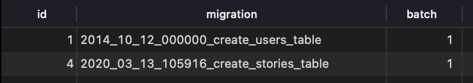
\includegraphics[scale=0.85]{resources/database/migrations-records}
    \caption{\mintinline{sql}|migrations| table.}
    \label{fig:migrations-records}
\end{figure}

The \mintinline{sql}|users| table (see Figure~\ref{fig:users-records}) contains all the information about user accounts, and it contains the following seven columns:

\begin{itemize}
    \item \mintinline{sql}|id|: the unique ID for each user account.
    \item \mintinline{sql}|name|: the name associated with user account.
    \item \mintinline{sql}|email|: the unique email used to log in.
    \item \mintinline{sql}|password|: the password used to log in, encrypted with 184 bit hashing by Bcrypt~\citep{laravel2022hashing}.
    \item \mintinline{sql}|remember_token|: keeps the user logged into the device if the user selects "Remember me".
    \item \mintinline{sql}|created_at|: records what date and time the user account was first created at.
    \item \mintinline{sql}|updated_at|: records what date and time the user account was last updated at.
\end{itemize}

\begin{figure}[!htbp]
    \centering
    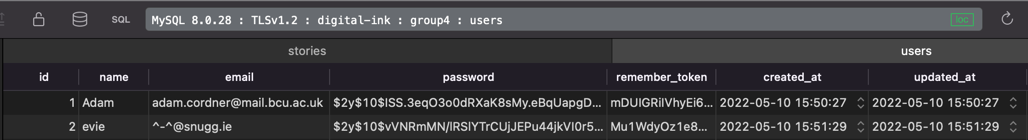
\includegraphics[scale=0.4]{resources/database/users-records}
    \caption{\mintinline{sql}|users| table.}
    \label{fig:users-records}
\end{figure}

The \mintinline{sql}|stories| table (see Figure~\ref{fig:stories-records}) contains all the information about user-created stories, and it contains the following 11 columns:

\begin{itemize}
    \item \mintinline{sql}|id|: the unique ID for each story.
    \item \mintinline{sql}|author_id|: the unique ID associated with the user who created the story.
    \item \mintinline{sql}|title|: the title associated with the story.
    \item \mintinline{sql}|genre|: the genre associated with the story, which can be one of eight different genres.
    \item \mintinline{sql}|blurb|: a brief description of the story.
    \item \mintinline{sql}|content|: the full content of the story.
    \item \mintinline{sql}|cover_image|: a thumbnail image for the story.
    \item \mintinline{sql}|file_upload|: an optional PDF upload of the story.
    \item \mintinline{sql}|published|: 1 if the story has been made public, or 0 if it is a draft.
    \item \mintinline{sql}|created_at|: records what date and time the story was first created at.
    \item \mintinline{sql}|updated_at|: records what date and time the story was last updated at.
\end{itemize}

\begin{figure}[!htbp]
    \centering
    \begin{subfigure}
        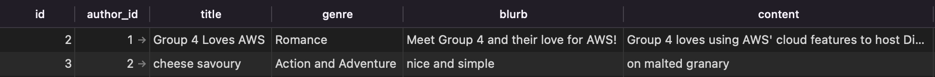
\includegraphics[scale=0.45]{resources/database/stories-records-1}
    \end{subfigure}
    \begin{subfigure}
        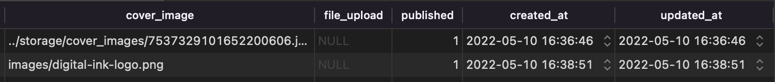
\includegraphics[scale=0.55]{resources/database/stories-records-2}
    \end{subfigure}
    \caption{\mintinline{sql}|stories| table.}
    \label{fig:stories-records}
\end{figure}

\section{Interface Design}\label{sec:interface}

The design of the web app was created using Blade, a powerful templating engine~\citep{laravel2022blade}.
When the user initially accesses the web app, they are able to log in or sign up.
This can be seen in Figure~\ref{fig:digital-ink-home-and-sign-up}.
When a user has created an account, a record is written to the \mintinline{sql}|users| table in the database.

\begin{figure}[!htbp]
    \centering
    \begin{minipage}{.5\textwidth}
        \centering
        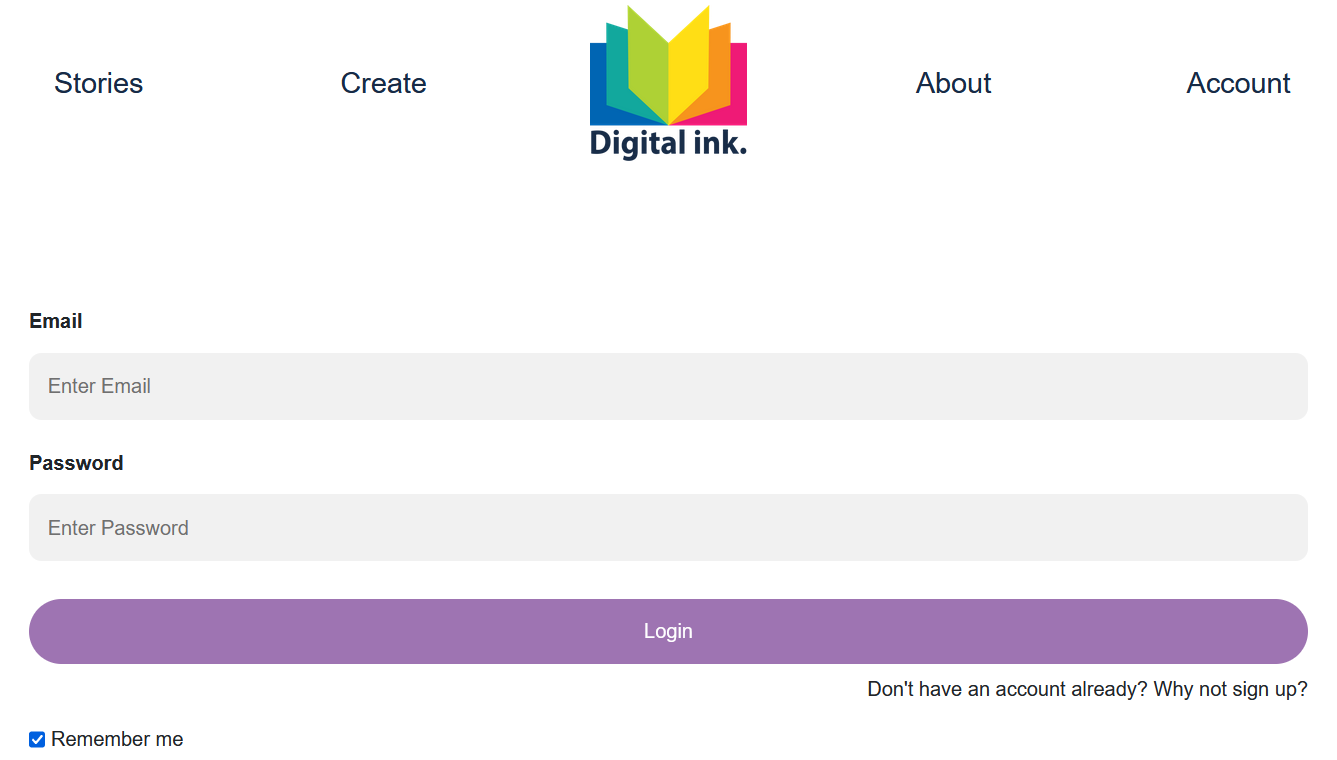
\includegraphics[width=1\linewidth]{resources/webapp/digital-ink-home}
        \label{fig:digital-ink-home}
    \end{minipage}%
    \begin{minipage}{.5\textwidth}
        \centering
        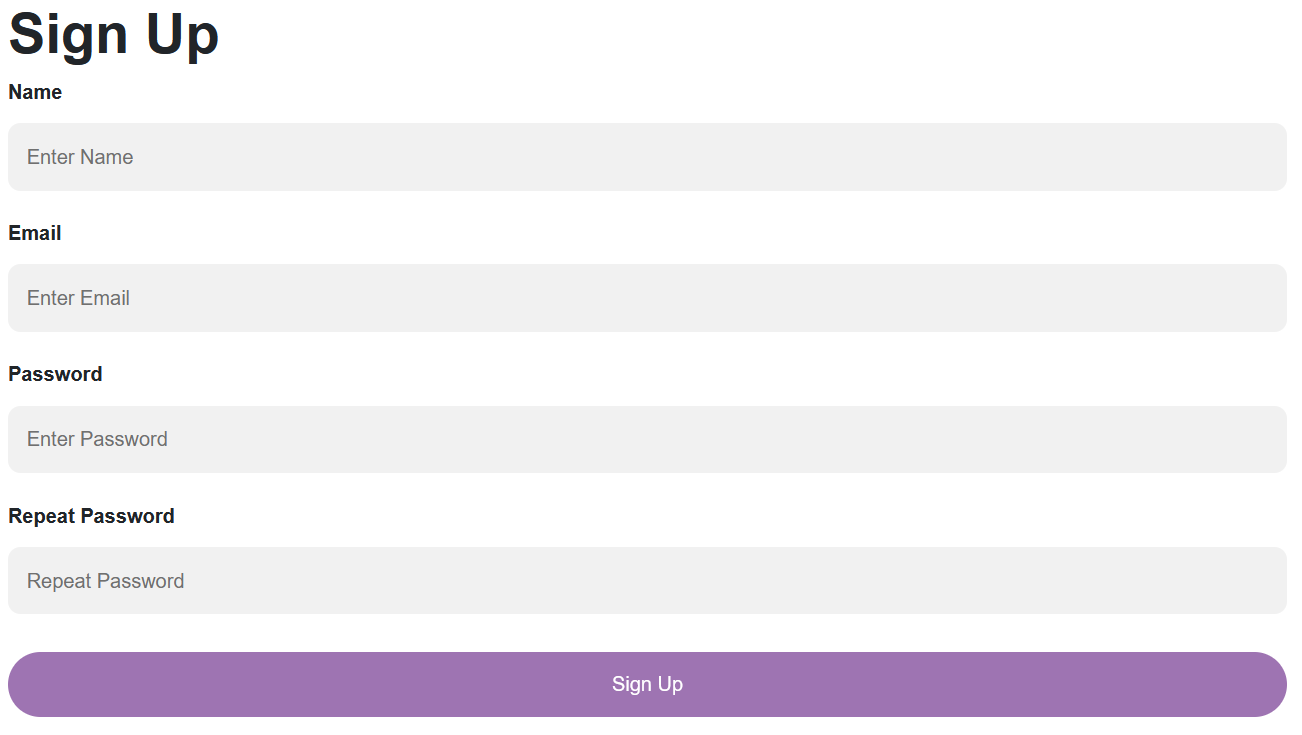
\includegraphics[width=1\linewidth]{resources/webapp/digital-ink-sign-up}
        \label{fig:digital-ink-sign-up}
    \end{minipage}
    \caption{\textit{Digital-Ink} home page log in and sign up forms.}
    \label{fig:digital-ink-home-and-sign-up}
\end{figure}

Once a user is signed in, they can create a story.
Creating a story requires the user to entire a title, a genre, the story itself, a blurb, and, optionally, a thumbnail image.
This can be seen in Figure~\ref{fig:digital-ink-create-story}.
Once a story has been created, it is written to the \mintinline{sql}|stories| table.

\begin{figure}[!htbp]
    \centering
        \begin{subfigure}
            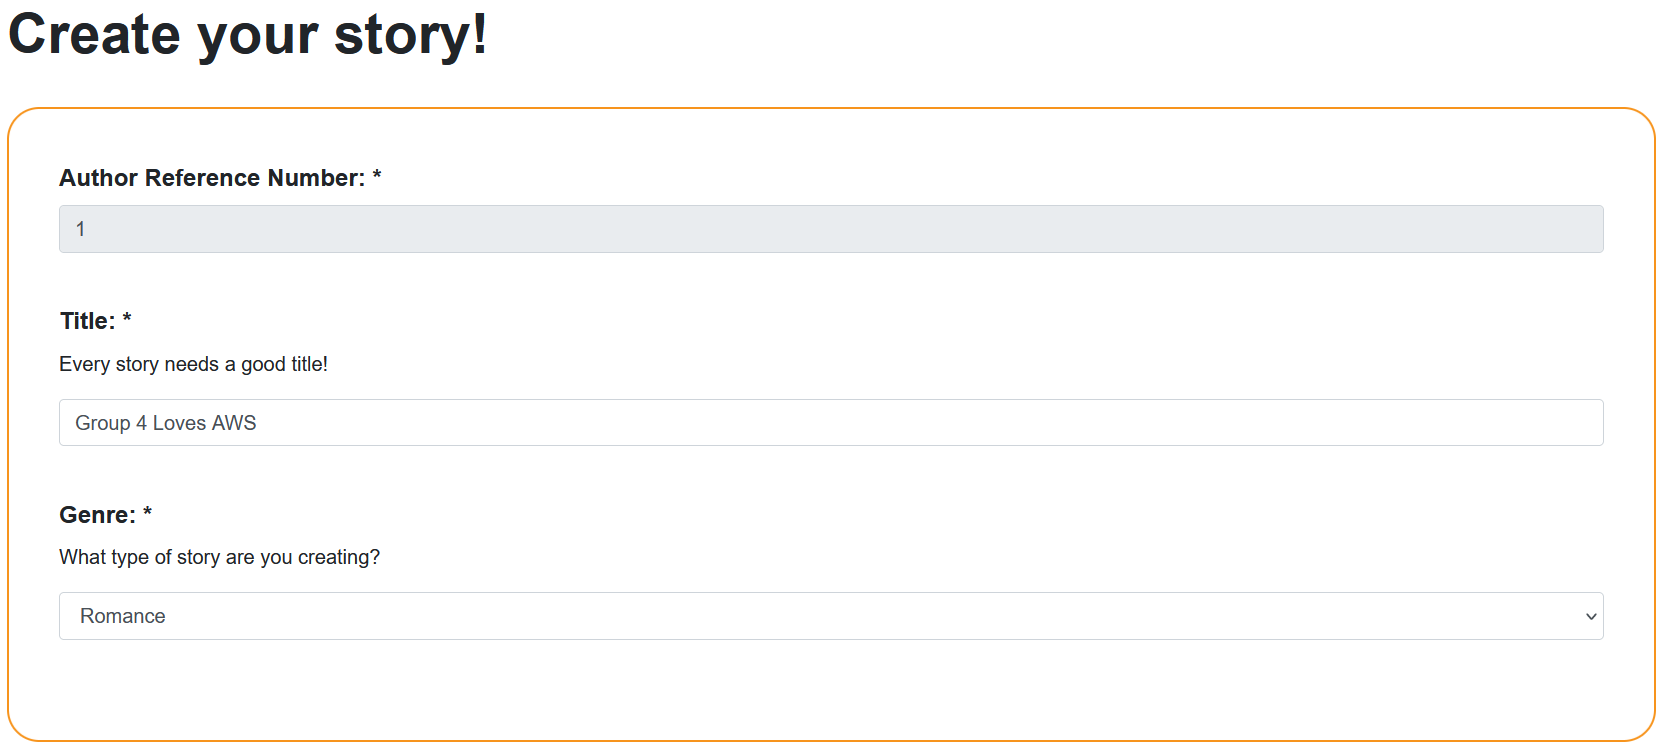
\includegraphics[scale=0.35]{resources/webapp/digital-ink-create-story-1}
        \end{subfigure}
        \begin{subfigure}
            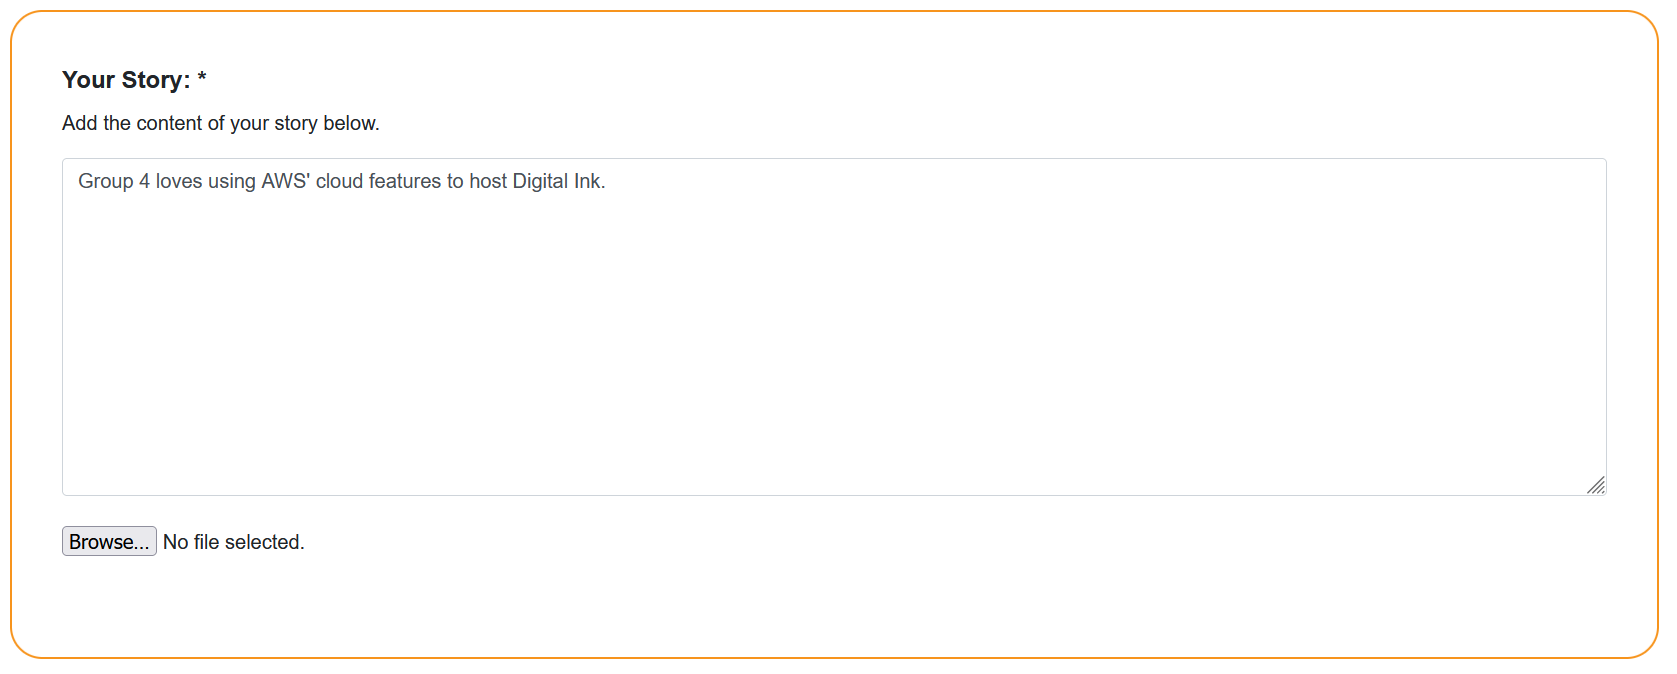
\includegraphics[scale=0.35]{resources/webapp/digital-ink-create-story-2}
        \end{subfigure}
        \begin{subfigure}
            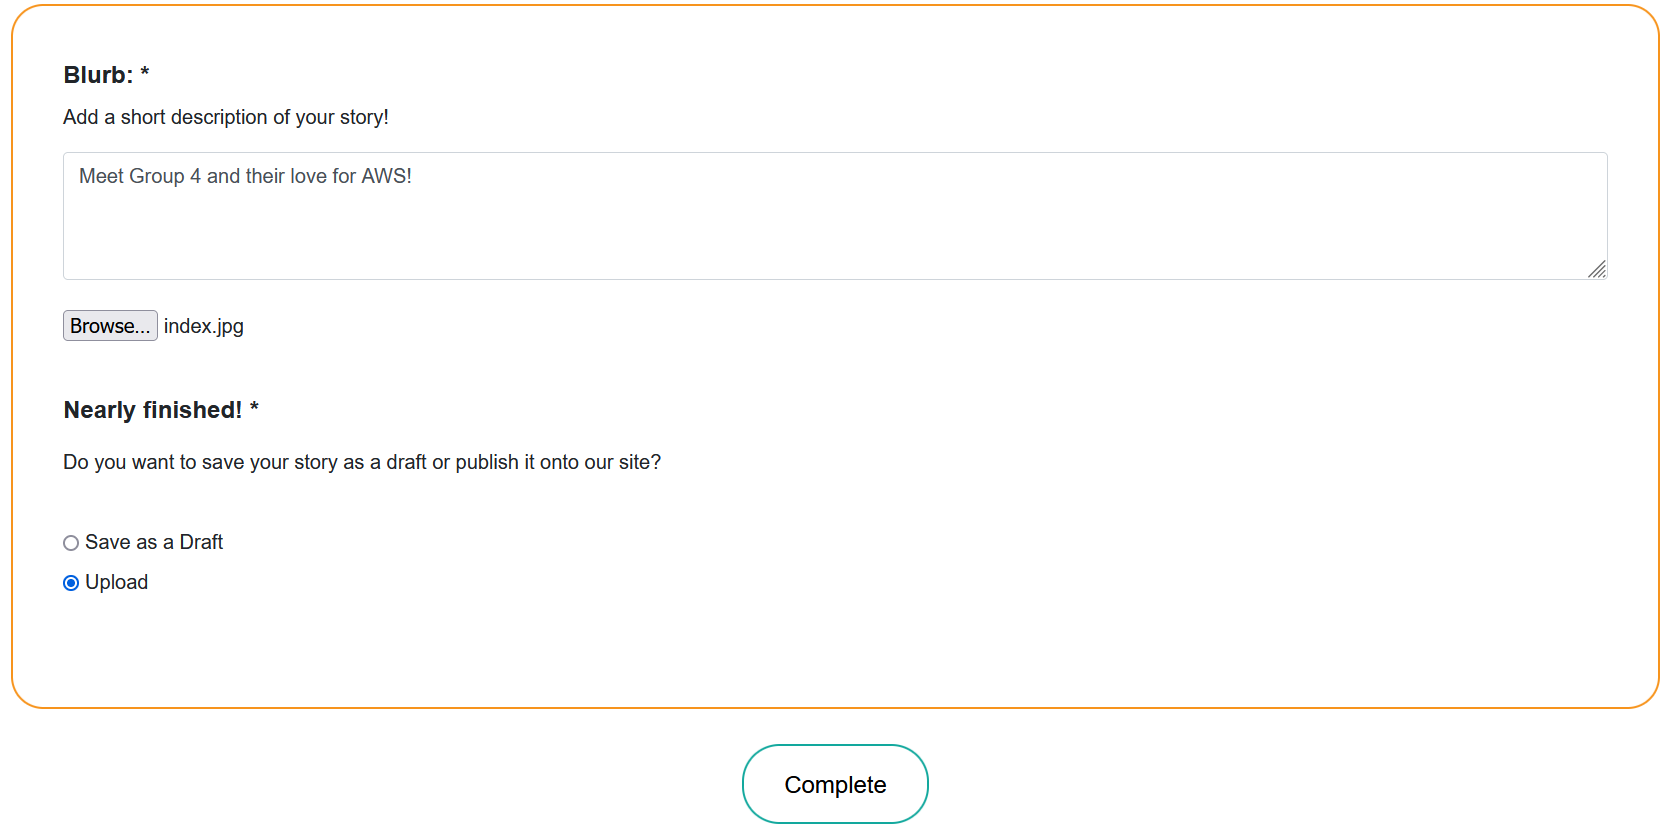
\includegraphics[scale=0.35]{resources/webapp/digital-ink-create-story-3}
        \end{subfigure}
        \caption{\textit{Digital-Ink} story creation form.}
        \label{fig:digital-ink-create-story}
\end{figure}

After this, the user can see all of their uploaded stories on their account page.
This can be seen in Figure~\ref{fig:digital-ink-account}.
From here, a story can be edited or deleted, which either updates a record in the \mintinline{sql}|stories|table or removes a record from it.

\begin{figure}[!htbp]
    \centering
        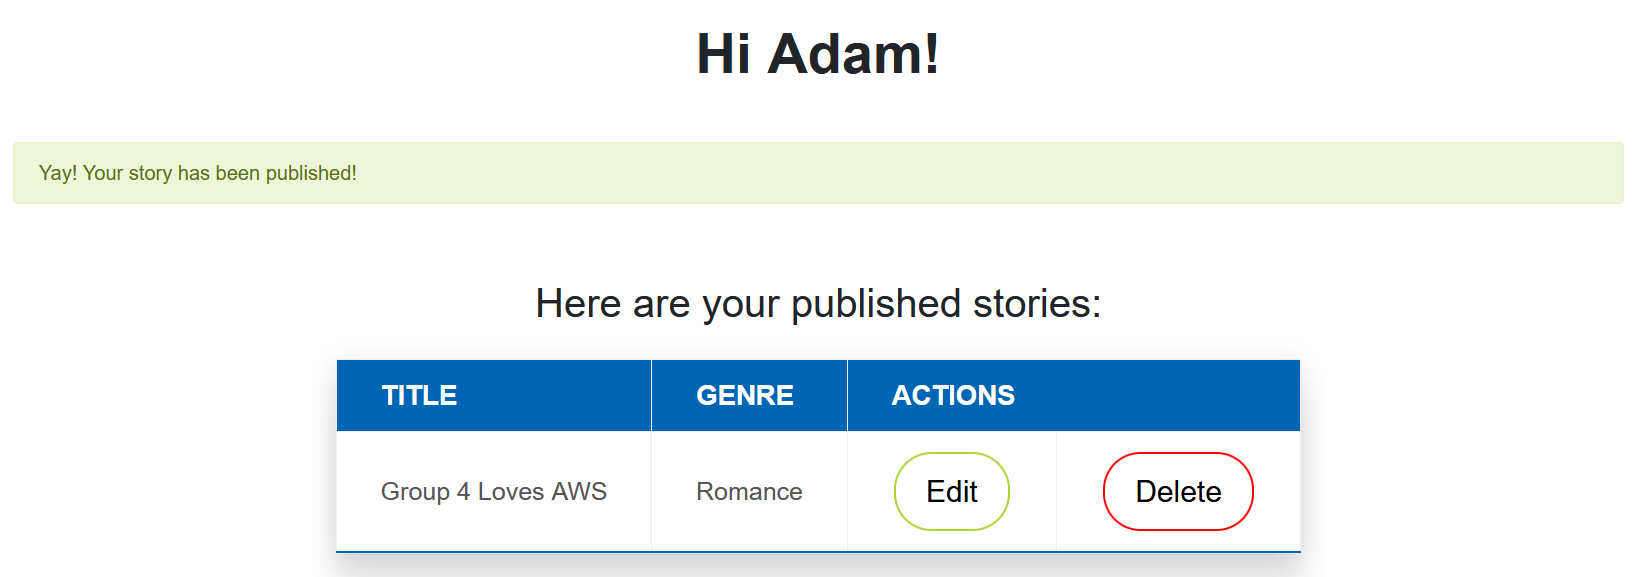
\includegraphics[scale=0.4]{resources/webapp/digital-ink-account}
        \caption{\textit{Digital-Ink} account page.}
        \label{fig:digital-ink-account}
\end{figure}

Lastly, on the Stories page, a user can view and search through all uploaded stories across all users.
Each story's title, genre, and blurb is shown in a list view.
A user can click into one of these stories to see the thumbnail image and read the full story.
These pages can be seen in Figure~\ref{fig:digital-ink-stories-and-story}.

\begin{figure}[!htbp]
    \centering
    \begin{subfigure}
        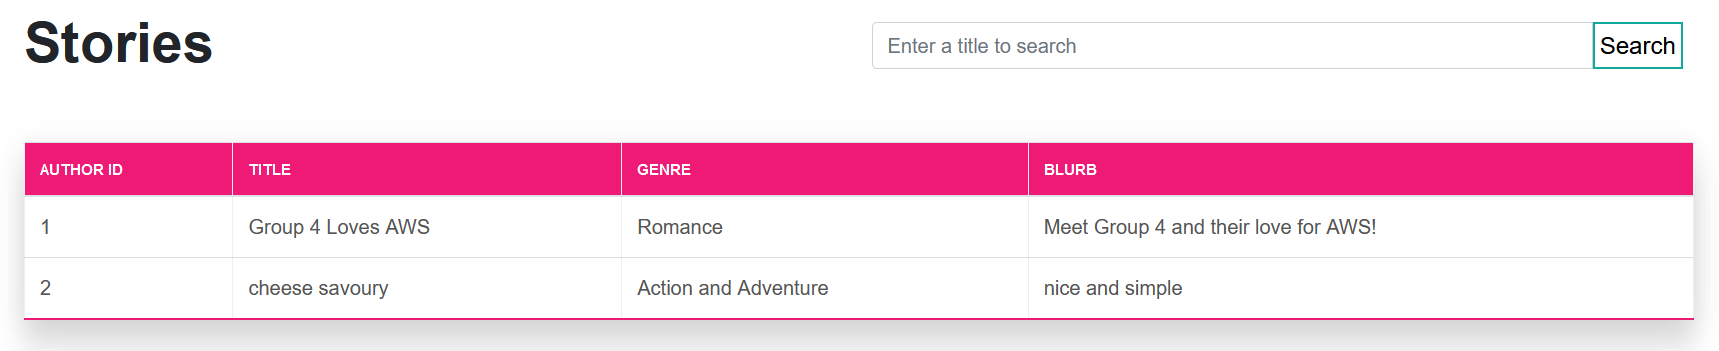
\includegraphics[scale=0.4]{resources/webapp/digital-ink-stories}
    \end{subfigure}
    \begin{subfigure}
        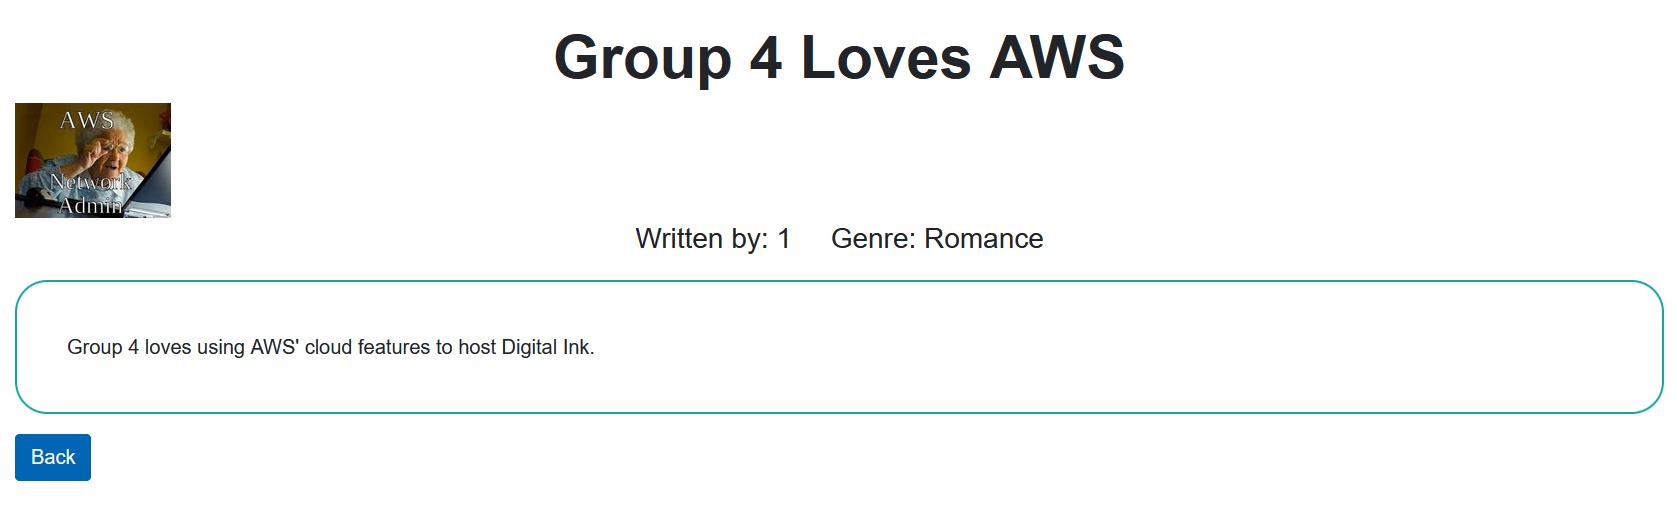
\includegraphics[scale=0.4]{resources/webapp/digital-ink-story}
    \end{subfigure}
    \caption{\textit{Digital-Ink} stories page and story view.}
    \label{fig:digital-ink-stories-and-story}
\end{figure}

    \chapter{Virtual Private Cloud (VPC)}\label{ch:vpc}

Amazon VPC allows for AWS resources to be launched in a virtual network that has been custom defined and configured.
This virtual network is similar to a traditional network which operates within your own physical data center, with the
added benefits of the scalable AWS infrastructure~\parencite{amazon2022what}.
A VPC can have multiple assigned subnets, which are a range of IP addresses accessible in the VPC\@.

The first step of migrating the web app to the cloud was creating a VPC to deploy and manage AWS resources for the app.
To do this, the VPC wizard must be used.
This is accessed by navigating to the VPC Management Console and then click the Launch VPC Wizard button, which can be
seen in Figure~\ref{fig:vpc-wizard}.

\begin{figure}[!htbp]
    \centering
    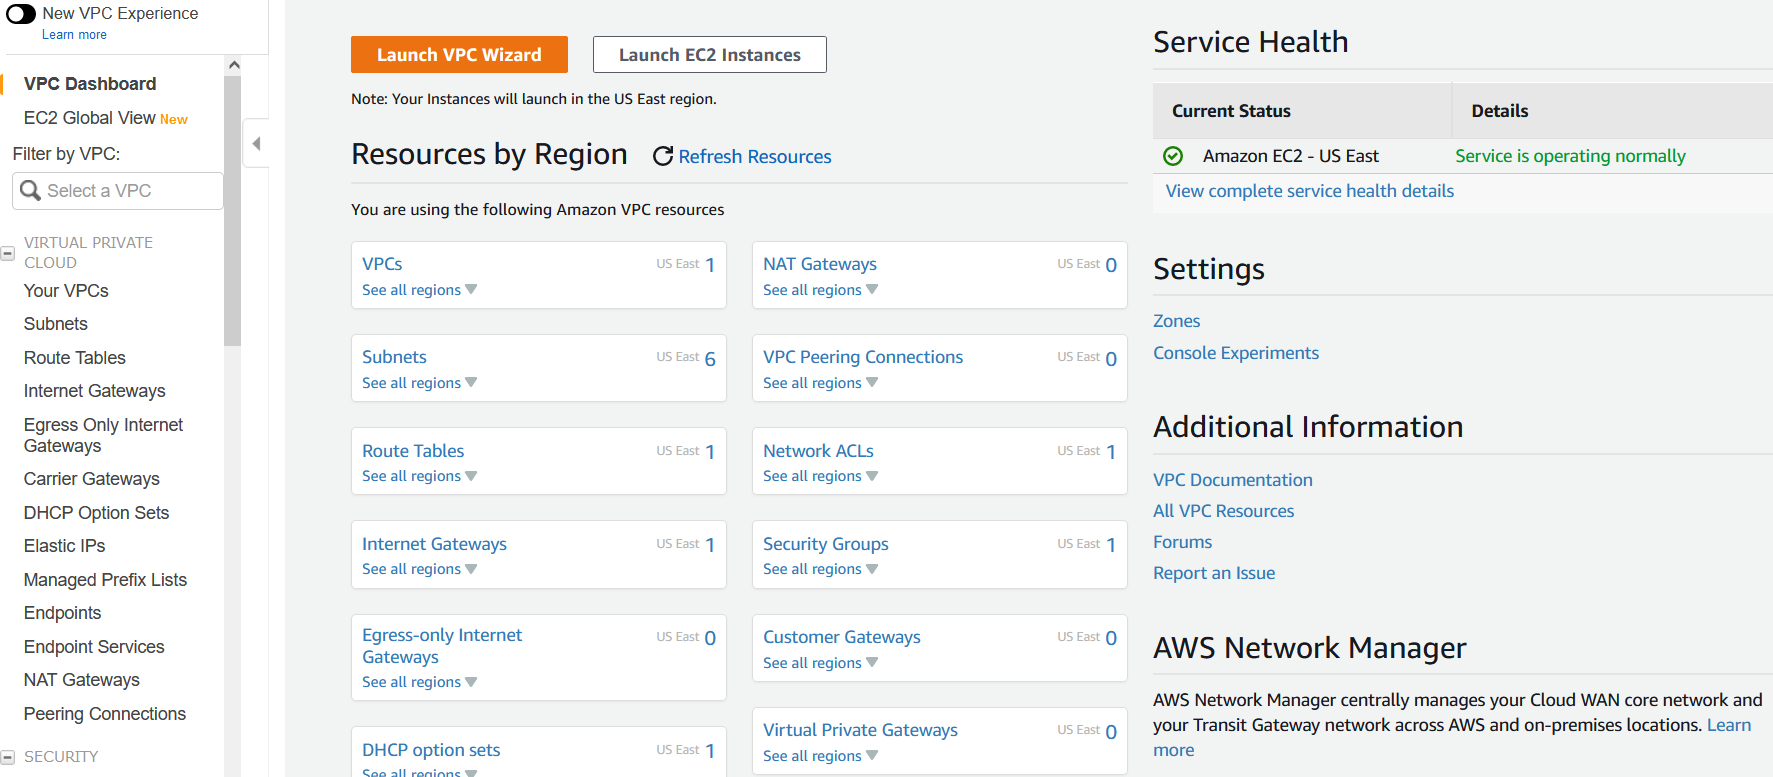
\includegraphics[width=\textwidth]{resources/vpc/vpc-dashboard}
    \caption{VPC Management Console.}
    \label{fig:vpc-wizard}
\end{figure}

The wizard presents us with step one of creating a VPC: selecting a VPC configuration.
There are several options for this, where each configuration has the following features:

\begin{itemize}
    \item VPC with a Single Public Subnet: Creates a /16 network with a /24 subnet where the subnet instances use
    Elastic IPs or Public IPs for internet access.
    \item VPC with Public and Private Subnets: Creates a /16 network and two /24 subnets where the public subnet
    instances use Elastic IPs for internet access and the private subnet instances use NAT for internet access.
    \item VPC with Public and Private Subnets and Hardware VPN Access: Creates a /16 network with two /24 subnets where
    one subnet is connected to the internet and another is connected to your personal network via a VPN\@.
    \item VPC with a Private Subnet Only and Hardware VPN Access: Creates a/16 network and a /24 subnet where the
    subnet is connected to your personal network via a VPN\@.
\end{itemize}

For the deployment of this web app, hardware VPN access is not necessary, so the VPC configuration with public and
private subnets was selected, as seen in Figure~\ref{fig:vpc-step-1}.

\begin{figure}[!htbp]
    \centering
    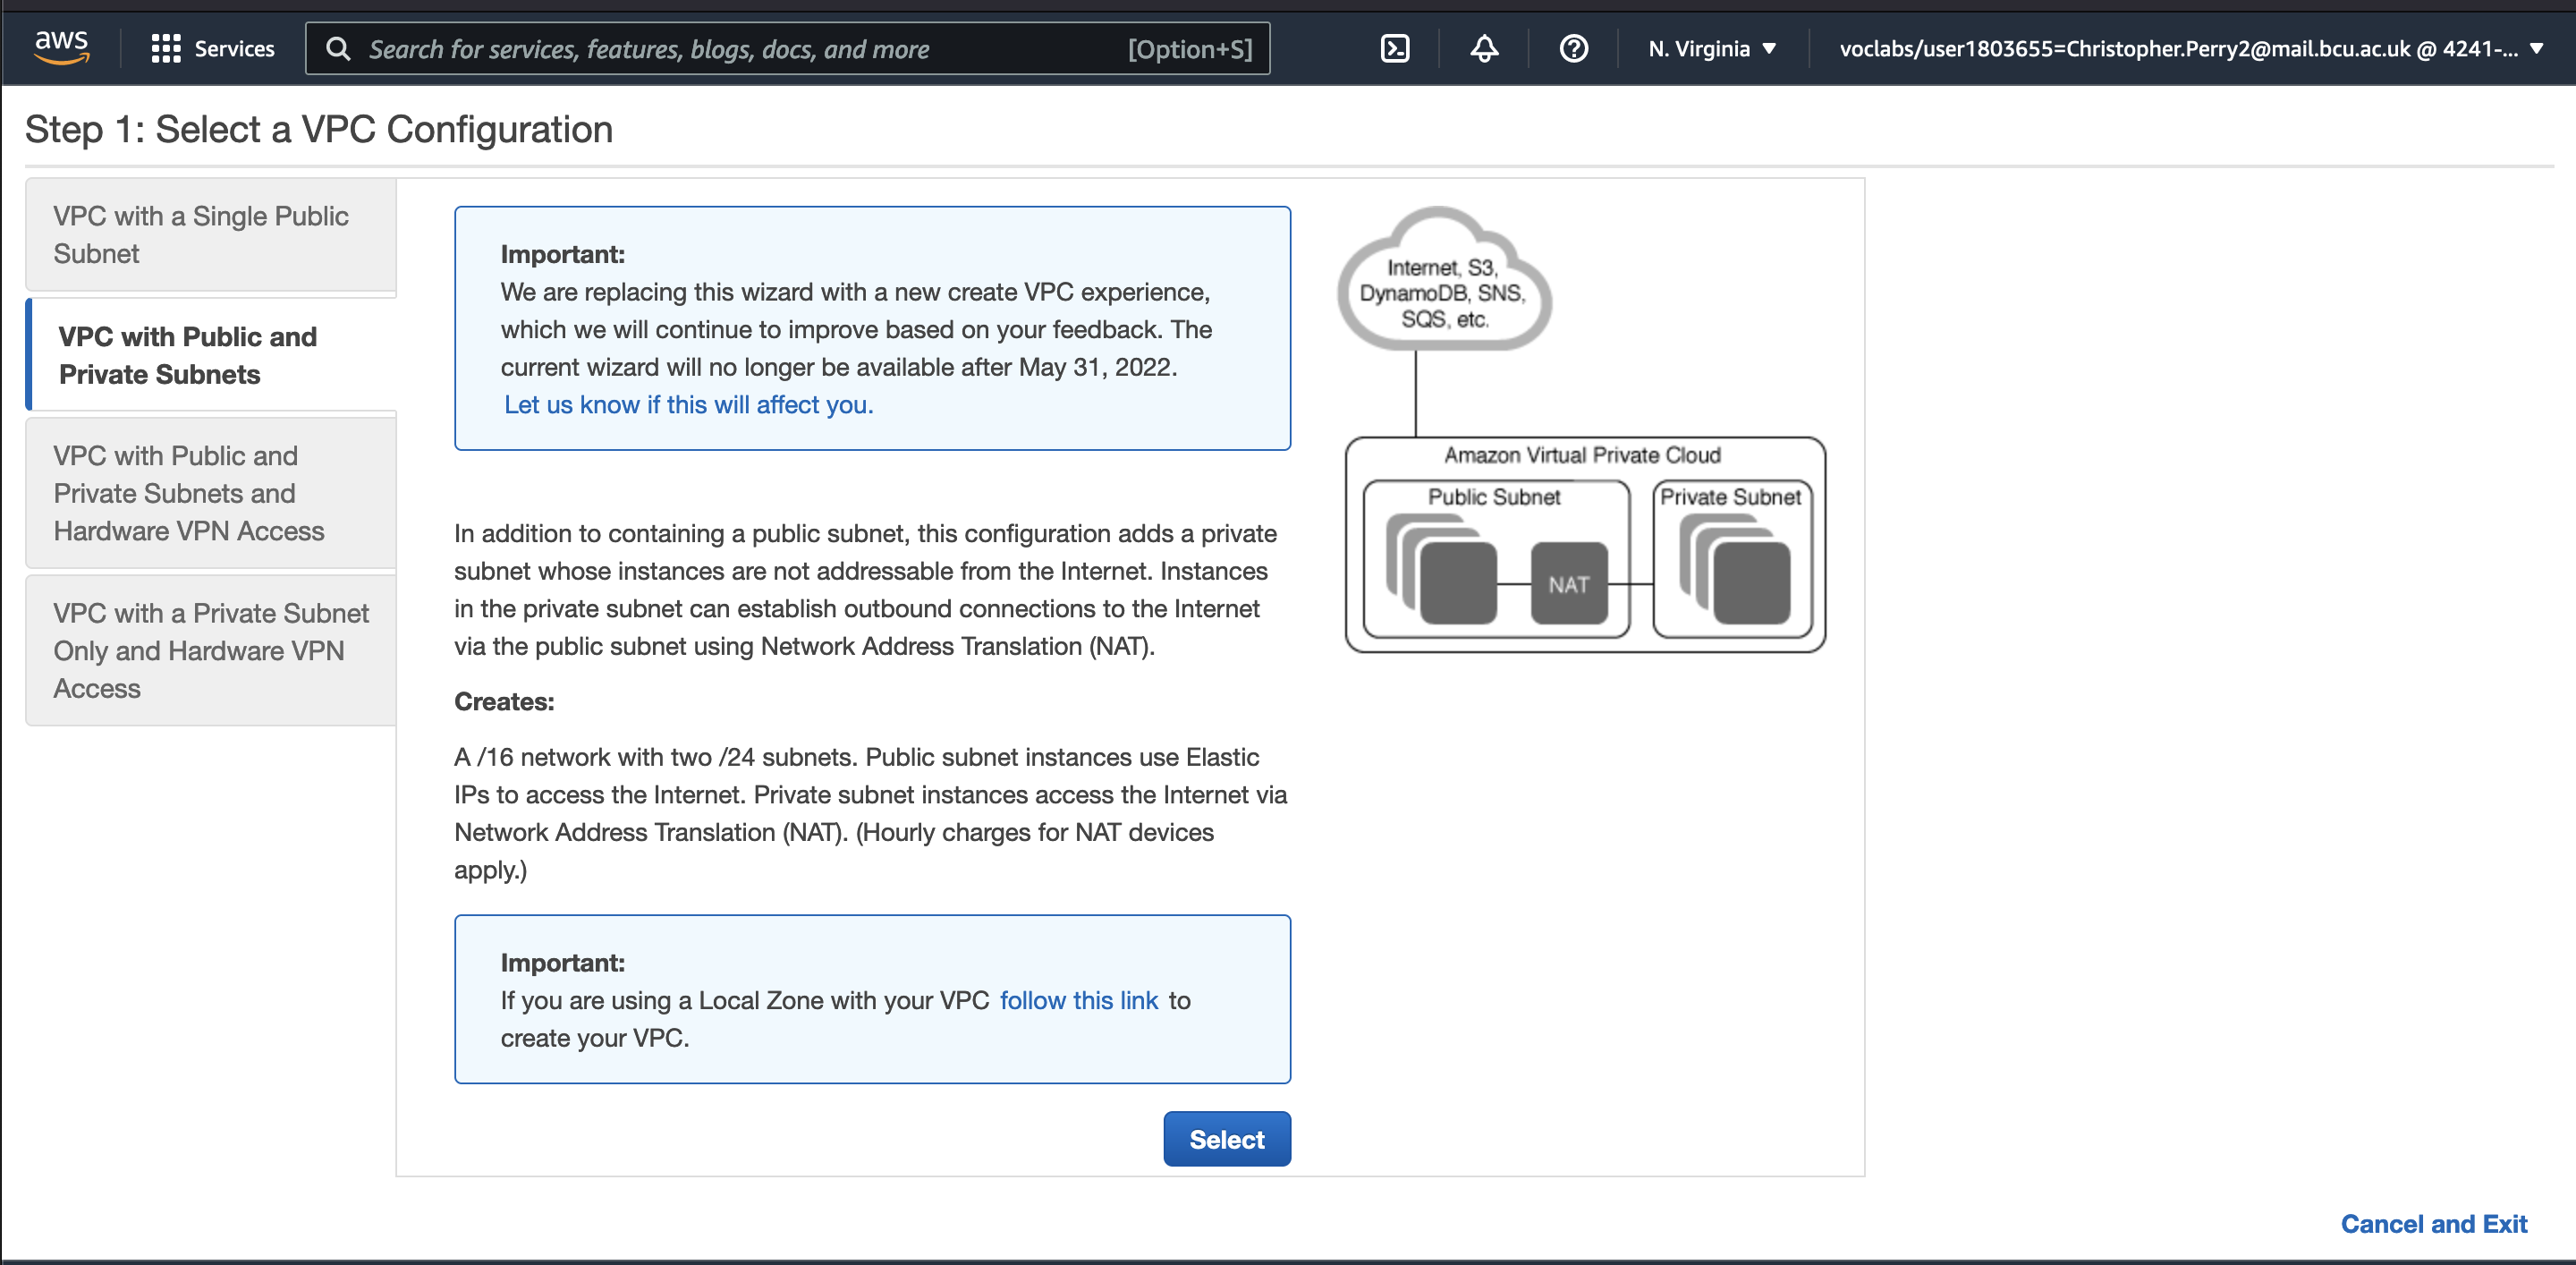
\includegraphics[width=\textwidth]{resources/vpc/step_1_select_a_vpc_configuration}
    \caption{Selecting a VPC configuration.}
    \label{fig:vpc-step-1}
\end{figure}

Following this, the specific details, such as the IP address block, of the selected configuration must be entered.
An IPv4 CIDR block of \mintinline{zsh}|10.0.0.0/16| was chosen as it provides a large amount of available IP addresses.
Additionally, no IPv6 CIDR block was configured and the VPC was named \mintinline{zsh}|Group4_VPC|.

Next, the public and private subnets were configured.
The public subnet was assigned an IPv4 CIDR of \mintinline{zsh}|10.0.0.0/24|, making 251 distinct IP addresses available
for the public subnet.
The availability zone of \mintinline{zsh}|us-east-1a| was chosen and the subnet was named
\mintinline{zsh}|Public subnet 1|.
The private subnet was assigned an IPv4 CIDR of \mintinline{zsh}|10.0.1.0/24|, making 251 distinct IP addresses
available for the private subnet as well.
The availability zone of \mintinline{zsh}|us-east-1a| was chosen and the subnet was named
\mintinline{zsh}|Private subnet 1|.

Lastly, the previously created Elastic IP Allocation ID was selected, and the remaining settings were left at their
default values.
Clicking the Create VPC button now will generate the VPC with the specified configurations.

\begin{figure}[!htbp]
    \centering
    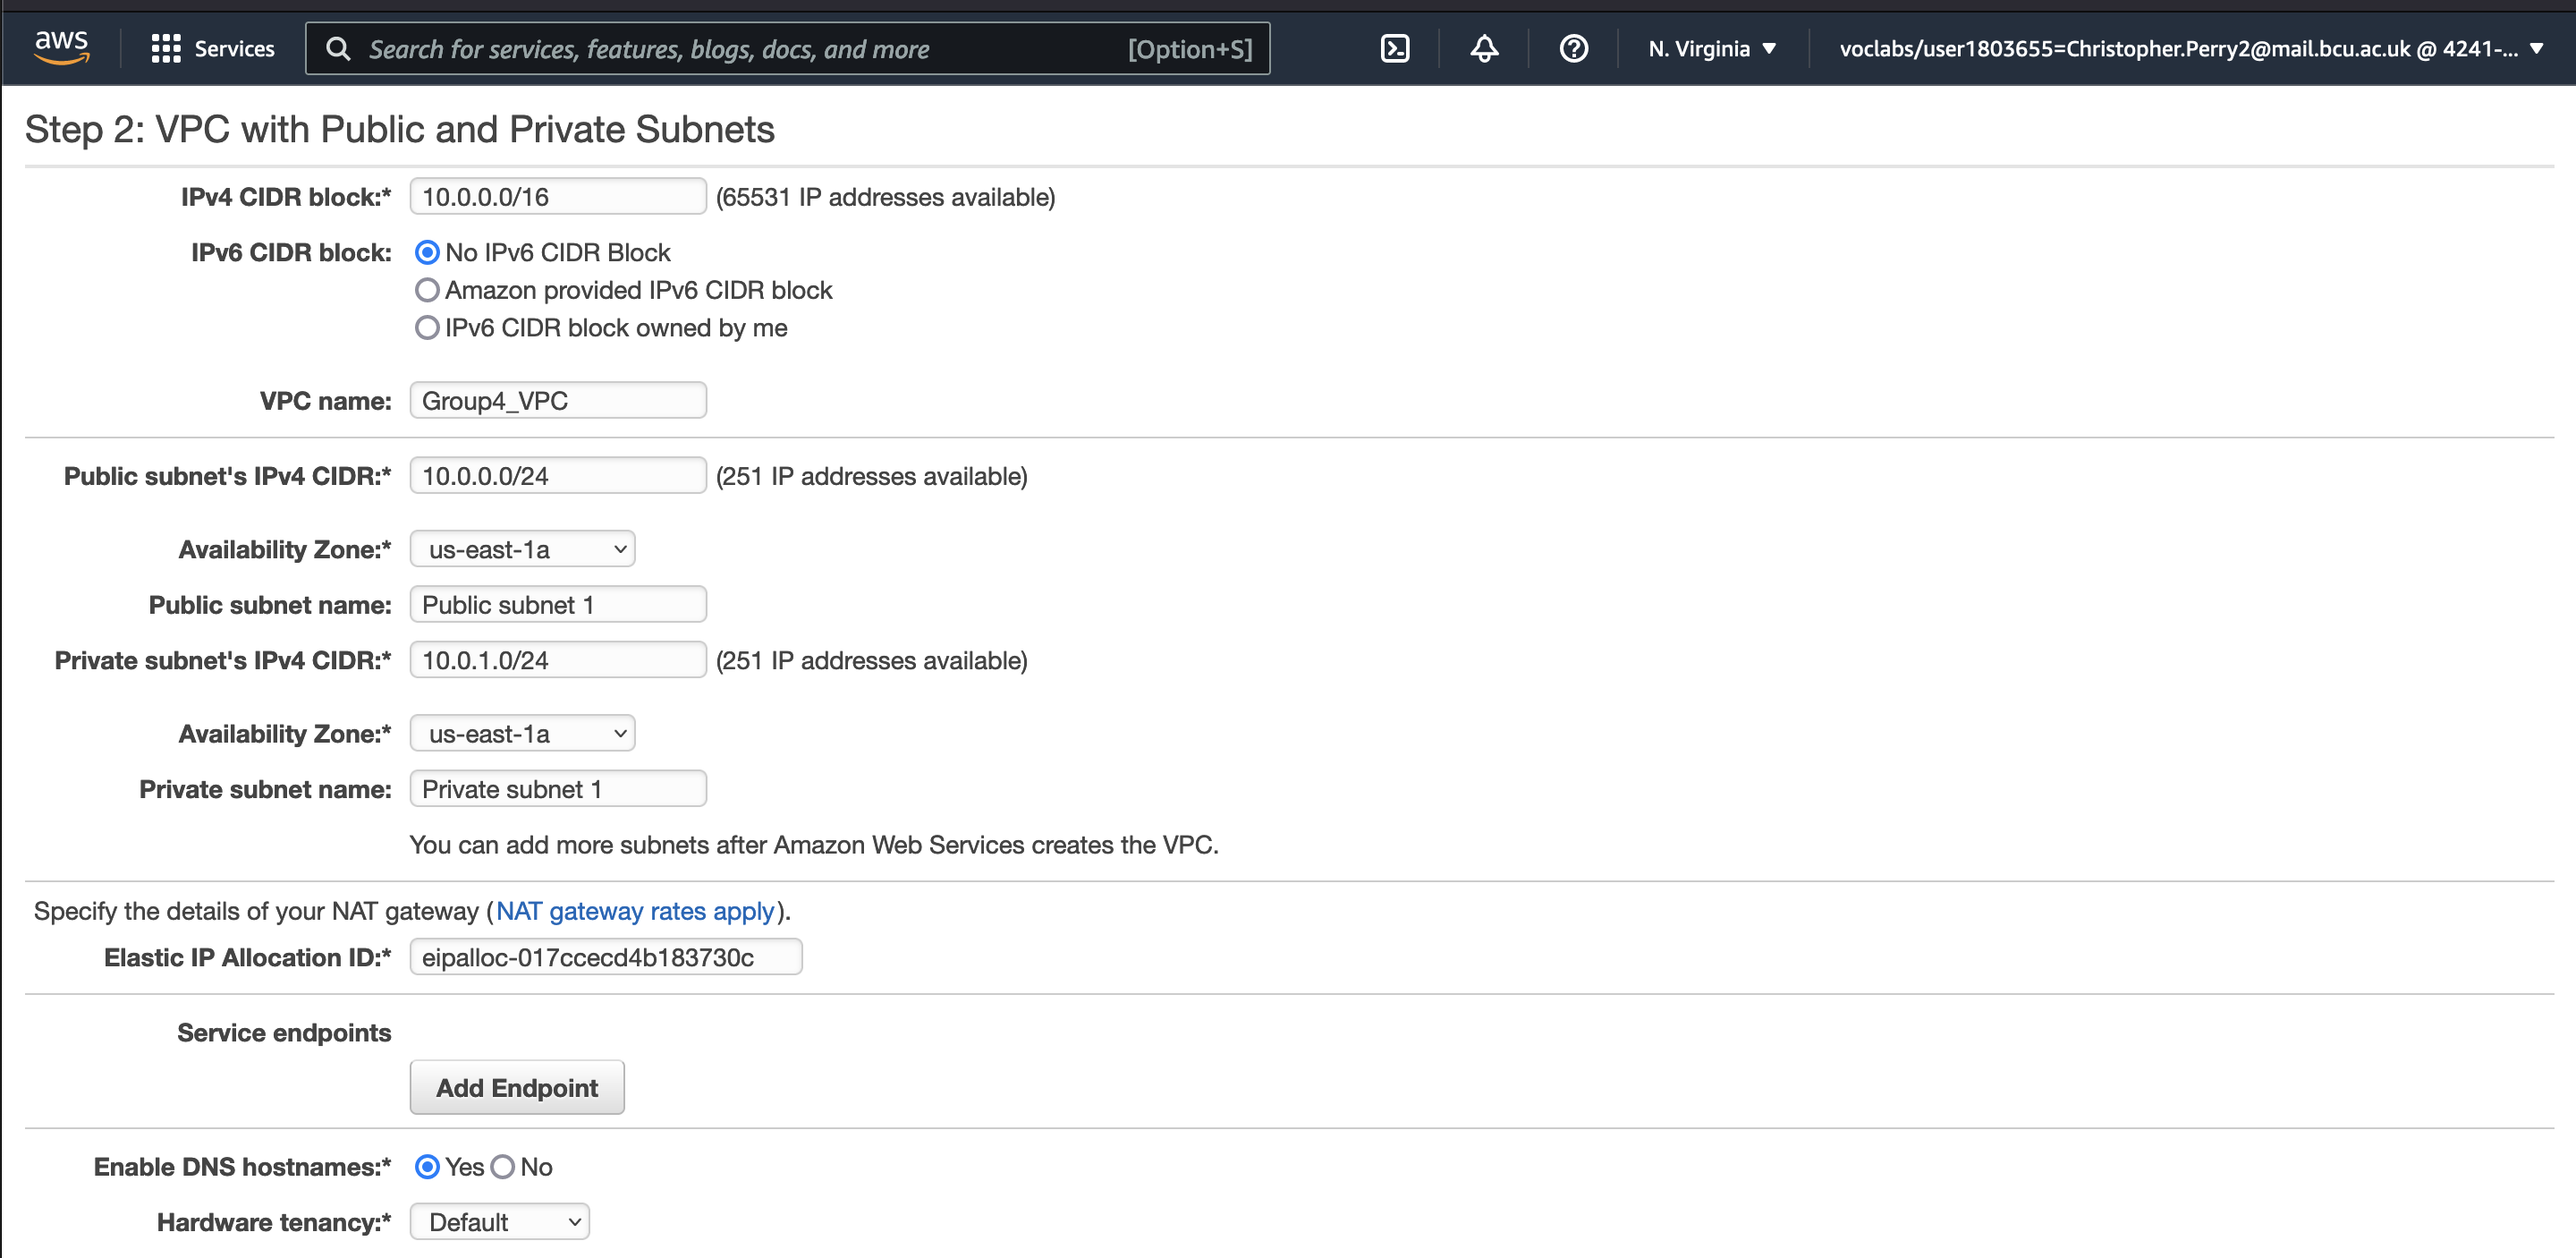
\includegraphics[width=\textwidth]{resources/vpc/step_2_vpc_with_public_and_private_subnets}
    \caption{Configuring VPC public and private subnets.}
    \label{fig:vpc-step-2}
\end{figure}

After this, AWS takes a few minutes to generate the VPC\@.

\begin{figure}[!htbp]
    \centering
    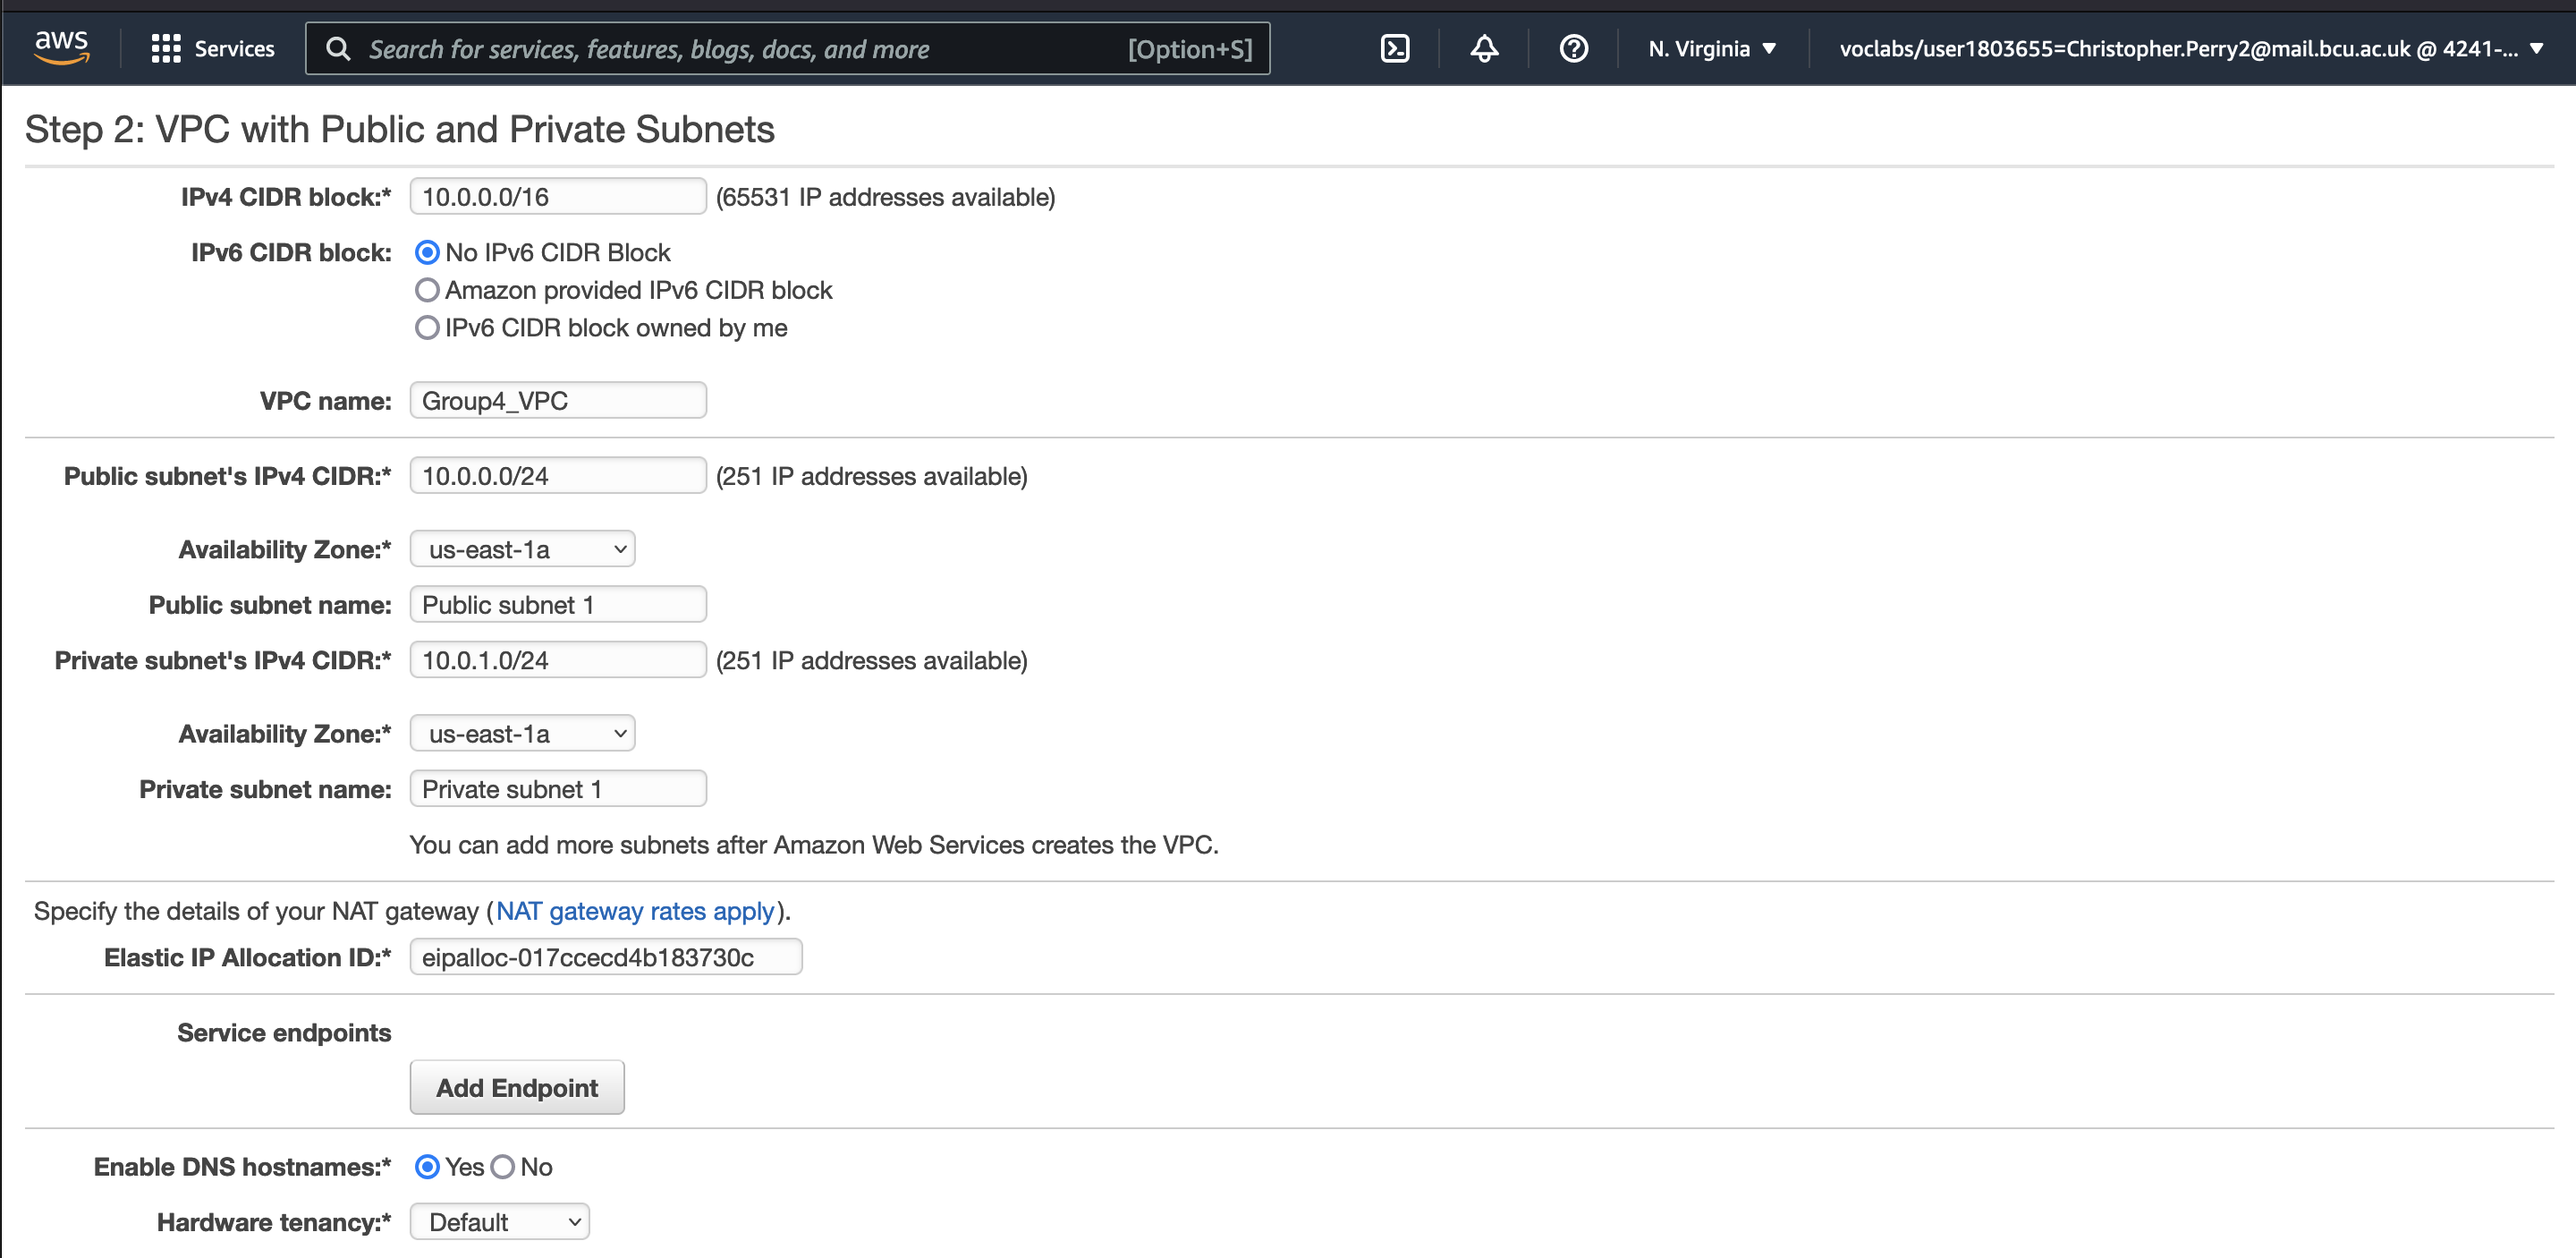
\includegraphics[width=\textwidth]{resources/vpc/step_2_vpc_with_public_and_private_subnets}
    \caption{Configuring VPC public and private subnets.}
    \label{fig:vpc-step-2}
\end{figure}
    \chapter{Elastic Cloud Compute}\label{ch:ec2}

\section{AWS Setup}\label{sec:aws-setup}

After the VPC and subnets were configured, the initial deployment of the web app began with setting up EC2.
This AWS service allows for scalable computing capacity through the use of a virtual computing environment hosted in the
cloud~\parencite{aws2022ec2}.
The web app will be stored on an EC2 instance of Amazon Linux, known as Amazon Machine Image (AMI), which will then be
launched through a docker container stored on the app.

\begin{figure}[!htbp]
    \centering
    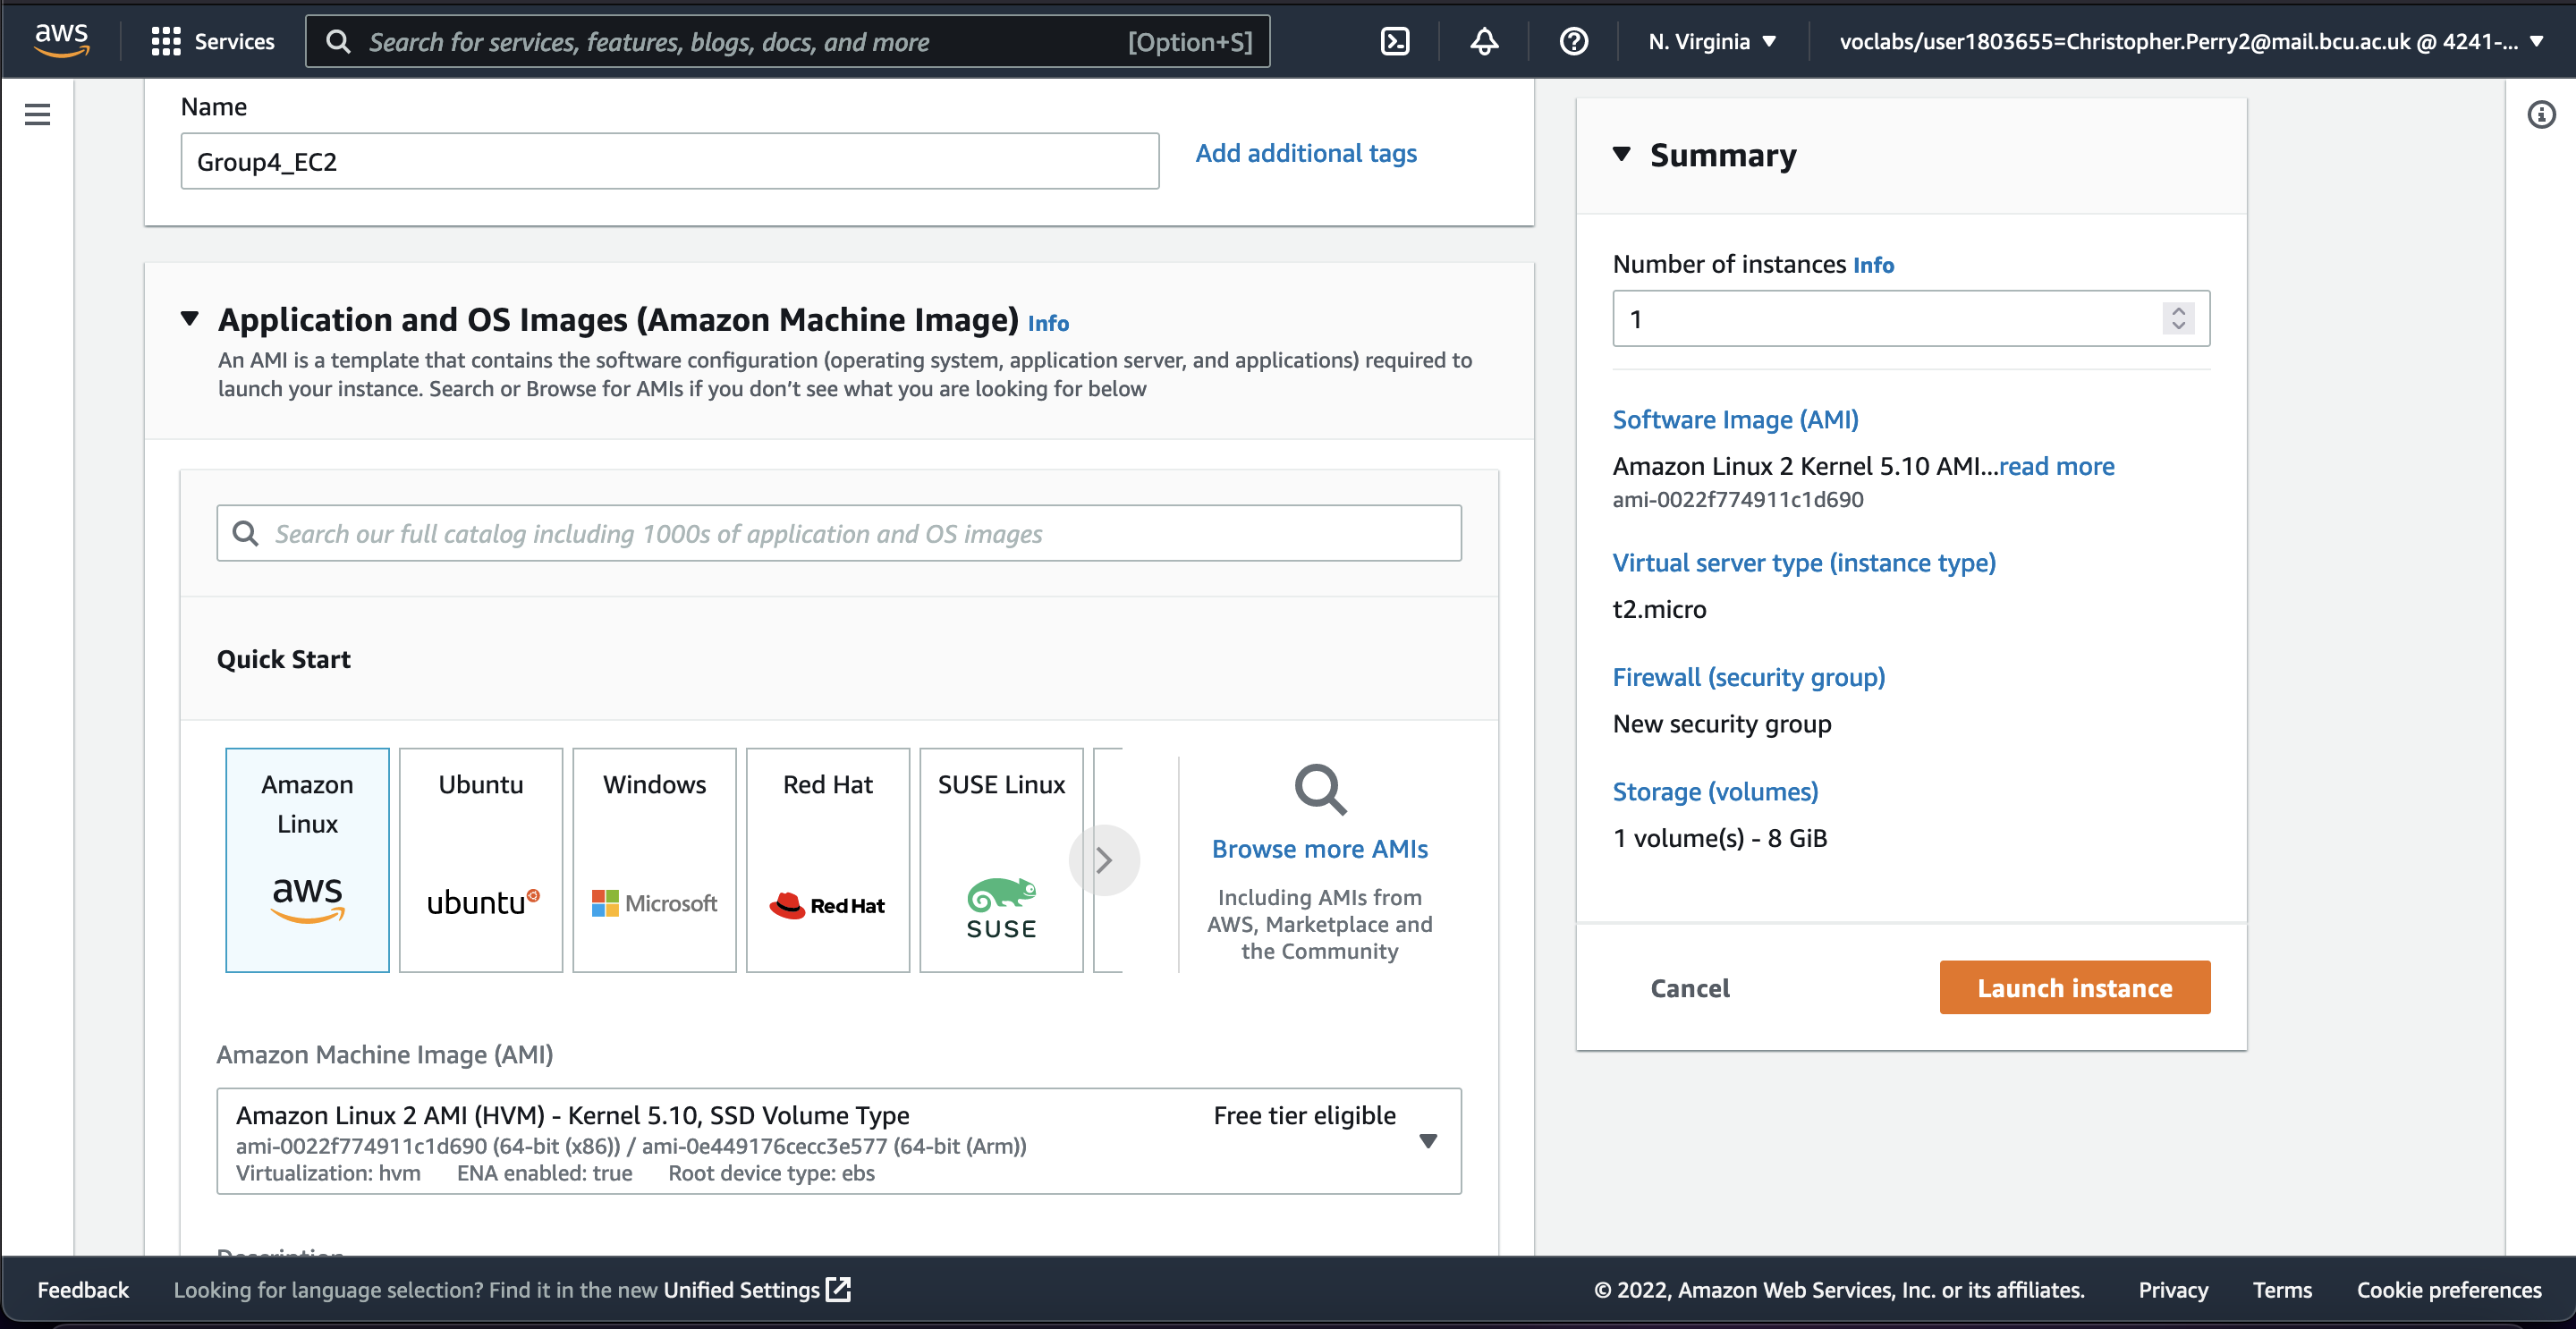
\includegraphics[width=\textwidth]{resources/ec2/create-instance-application-and-os-images}
    \caption{Selection of EC2 OS Image.}
    \label{fig:ec2-os}
\end{figure}

Figure~\ref{fig:ec2-os} details the selection of the Operating System (OS) that will be used for the EC2 instance.
The \textit{Amazon Linux 2} AMI was selected, as it is already configured with Linux and does not need any more setup.

\clearpage
Now that an AMI has been chosen, the specific instance type that will be used within this AMI can be selected.
It was decided that the instance type of \textit{t2.micro} would be used, as it contains only 1GB of Random Access
Memory (RAM).
The selection of this can be found in Figure~\ref{fig:ec2-instance}.

\begin{figure}[!htbp]
    \centering
    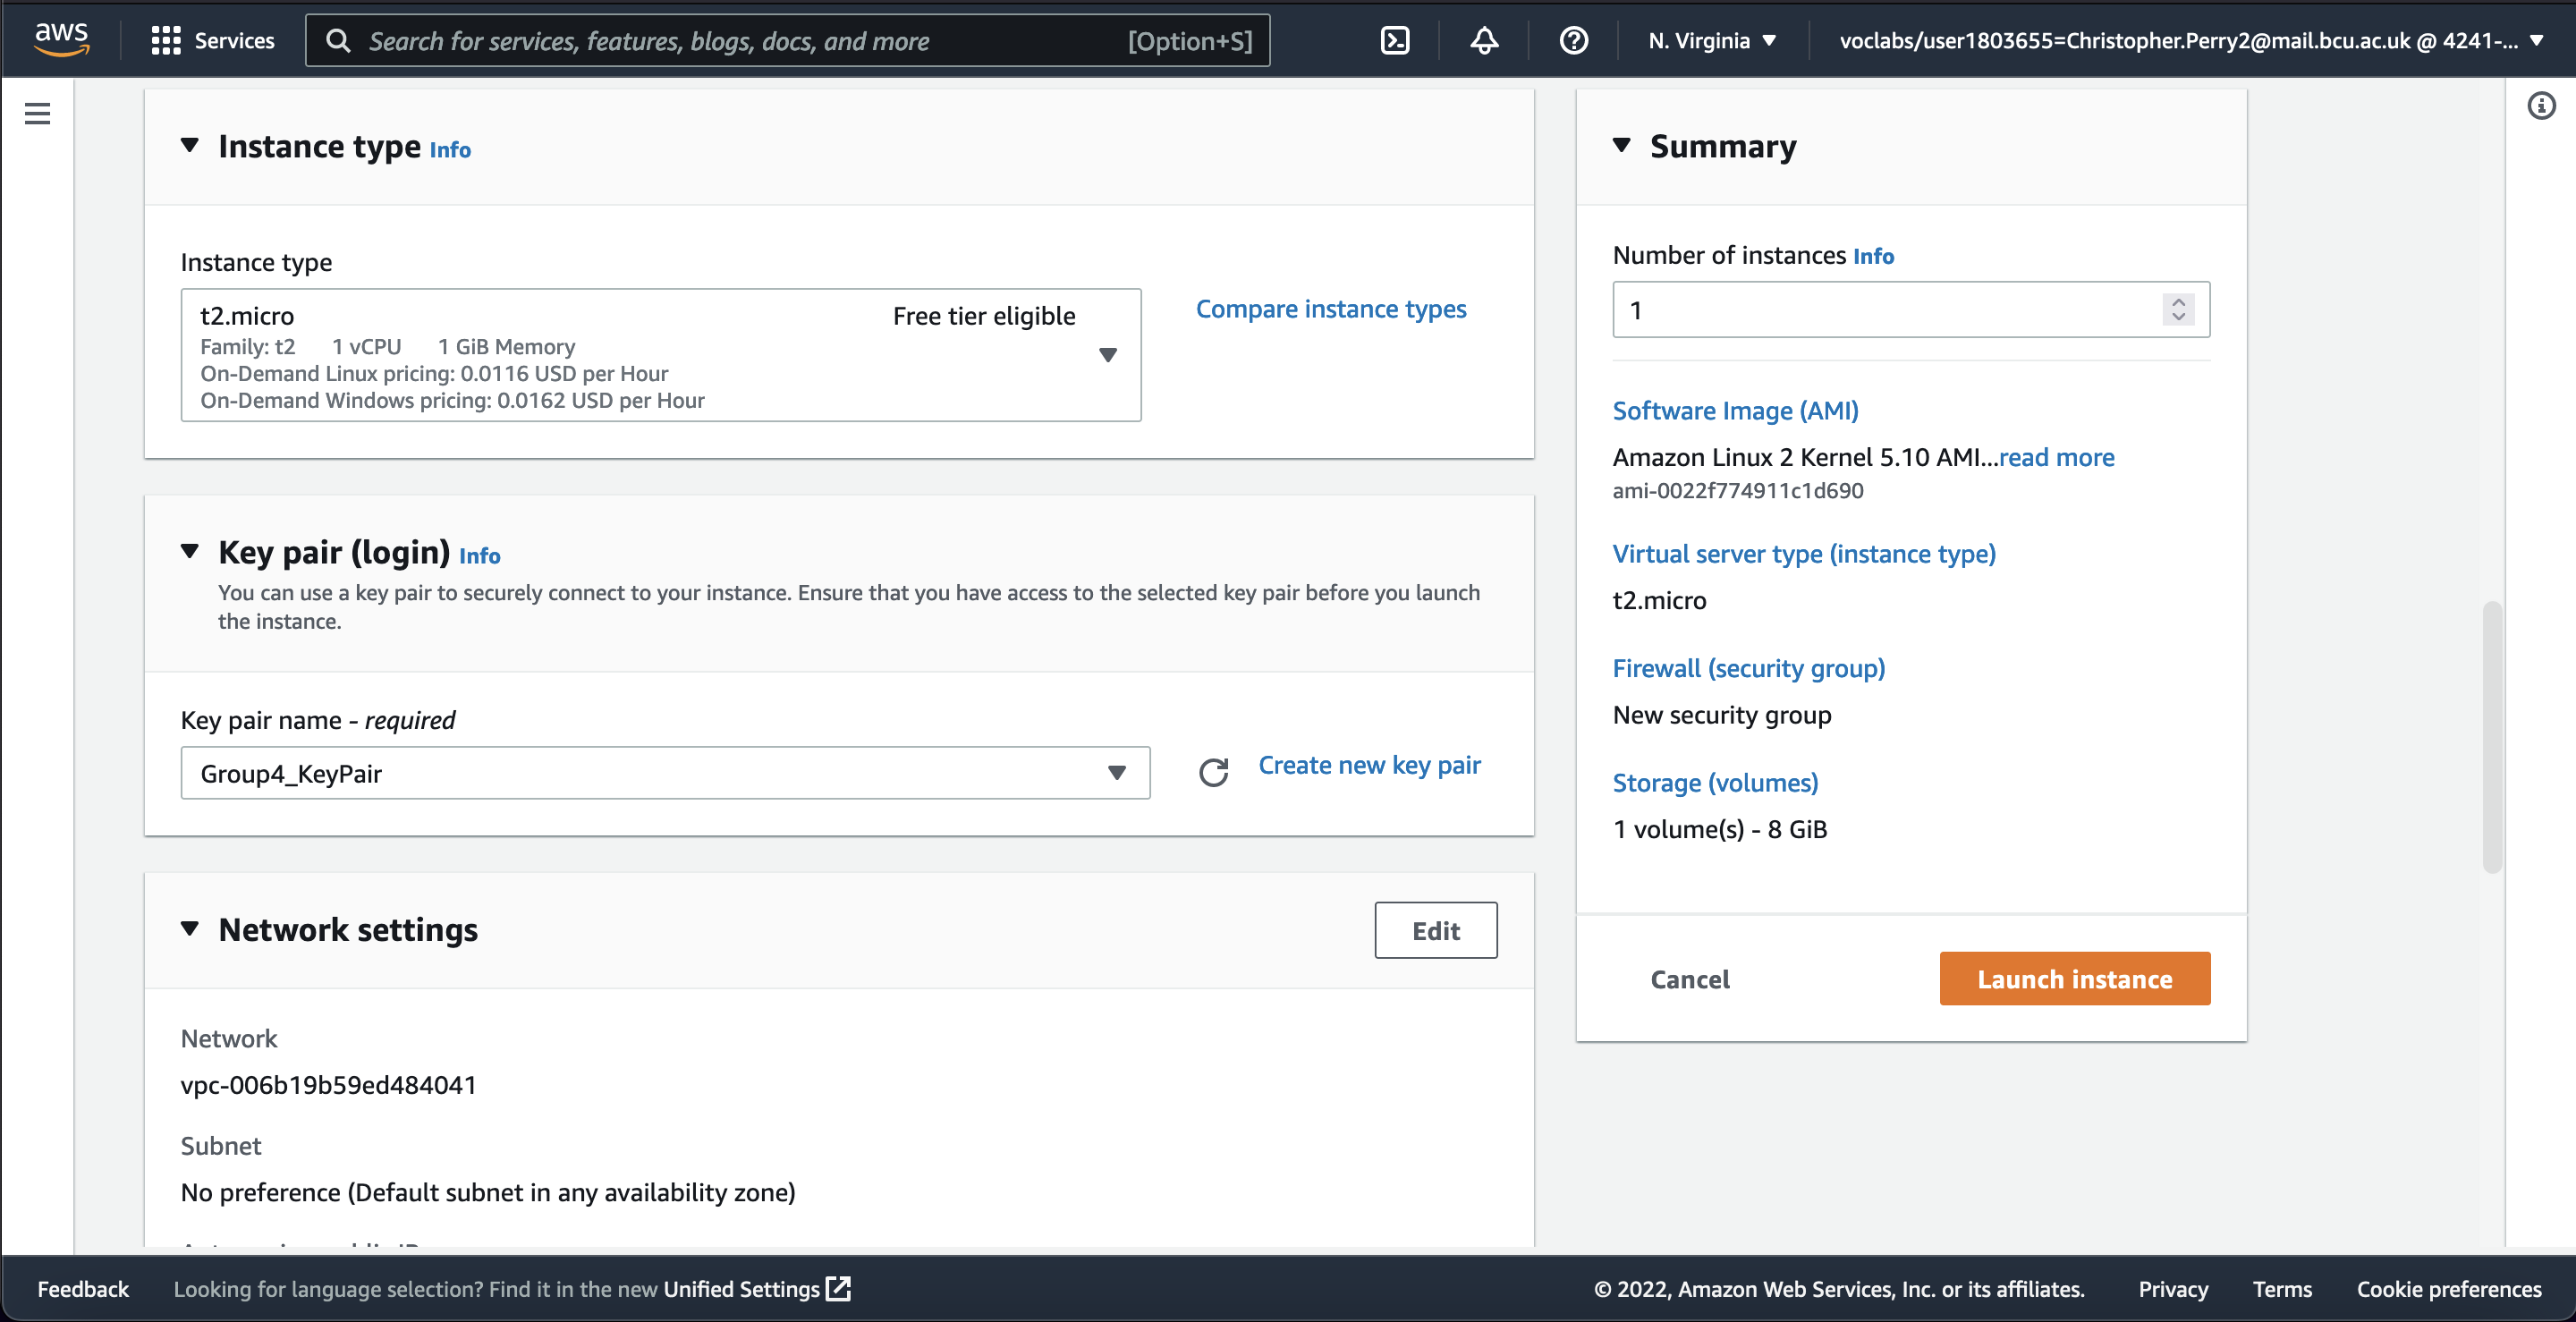
\includegraphics[width=\textwidth]{resources/ec2/create-instance-instance-type}
    \caption{Selection of EC2 Instance.}
    \label{fig:ec2-instance}
\end{figure}

A key pair will allow for the ability to sign in to the EC2 instance with a unique set of login credentials, heightening
the security of the project.

The next stage of the setup process was to set up networking for the EC2 instance, in order for the web app to work with
Docker to download relevant containers from DockerHub, which will allow a Laravel instance to be initialised, as
discussed in Section~\ref{ch:web-app}.

\begin{figure}[!htbp]
    \centering
    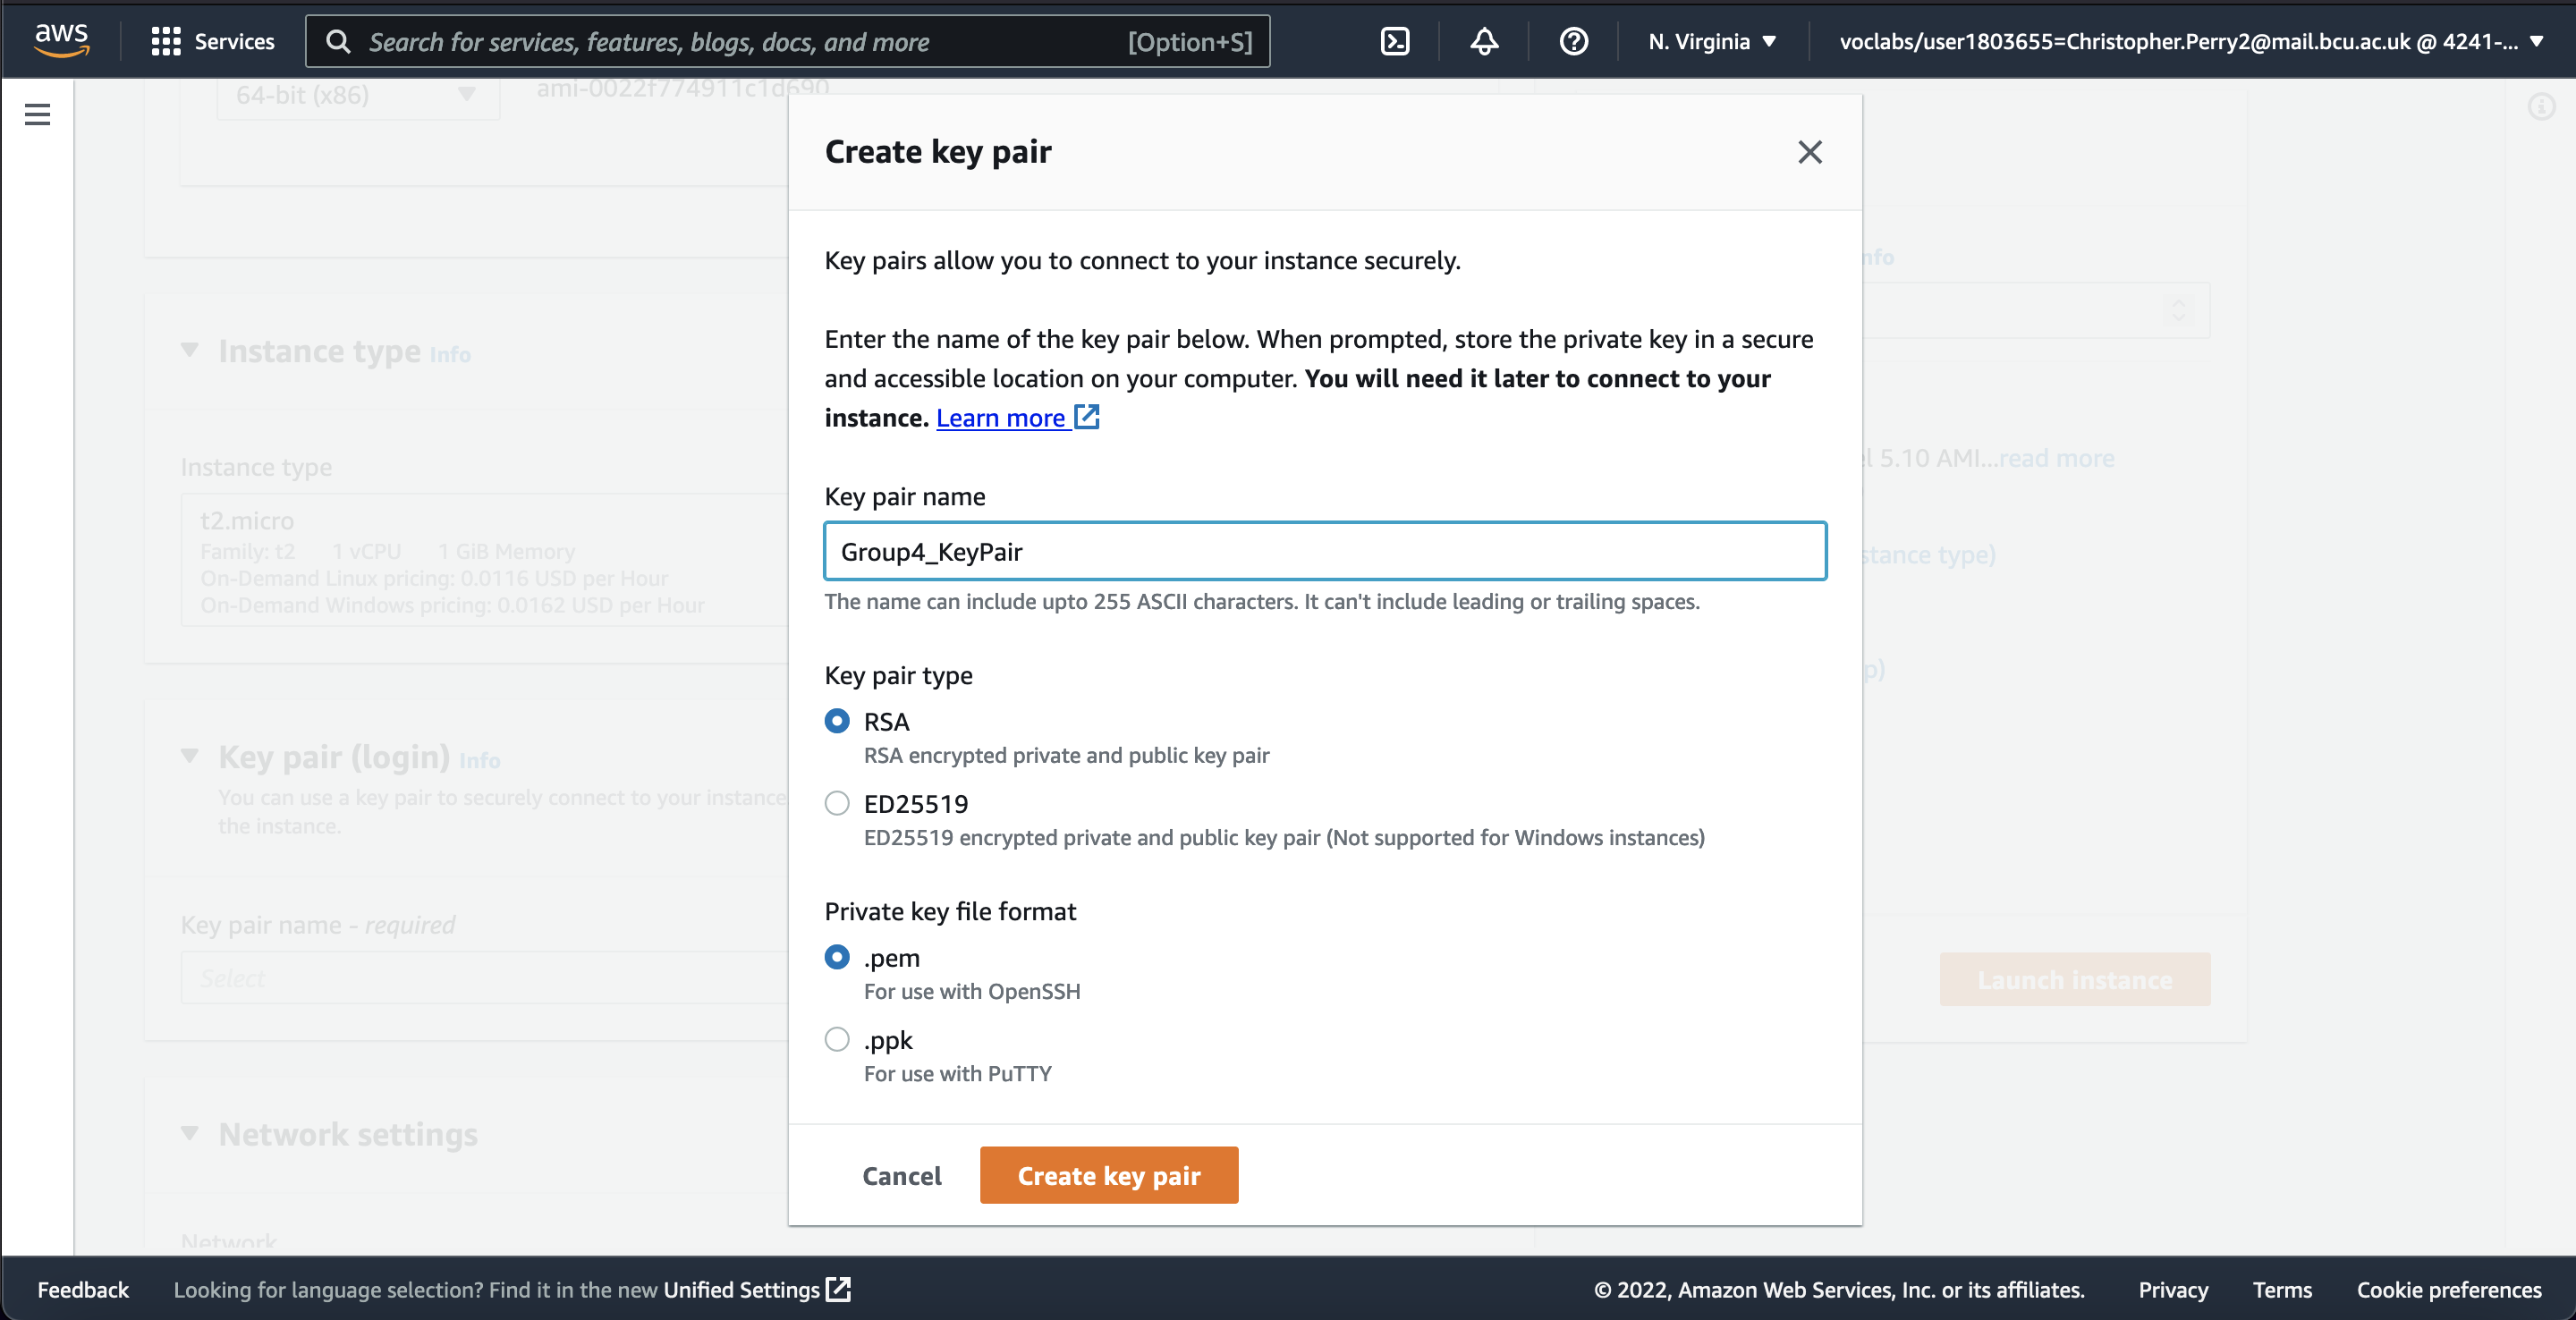
\includegraphics[width=\textwidth]{resources/ec2/create-key-pair}
    \caption{Selection of EC2 Keypair.}
    \label{fig:ec2-keypair}
\end{figure}

This process can be seen in Figure~\ref{fig:ec2-keypair}.

The instance is assigned the VPC created in Section~\ref{ch:vpc-subnets}, where it is assigned a subnet in the same
availability zone of \mintinline{zsh}|us-east-1|.

\begin{figure}[!htbp]
    \centering
    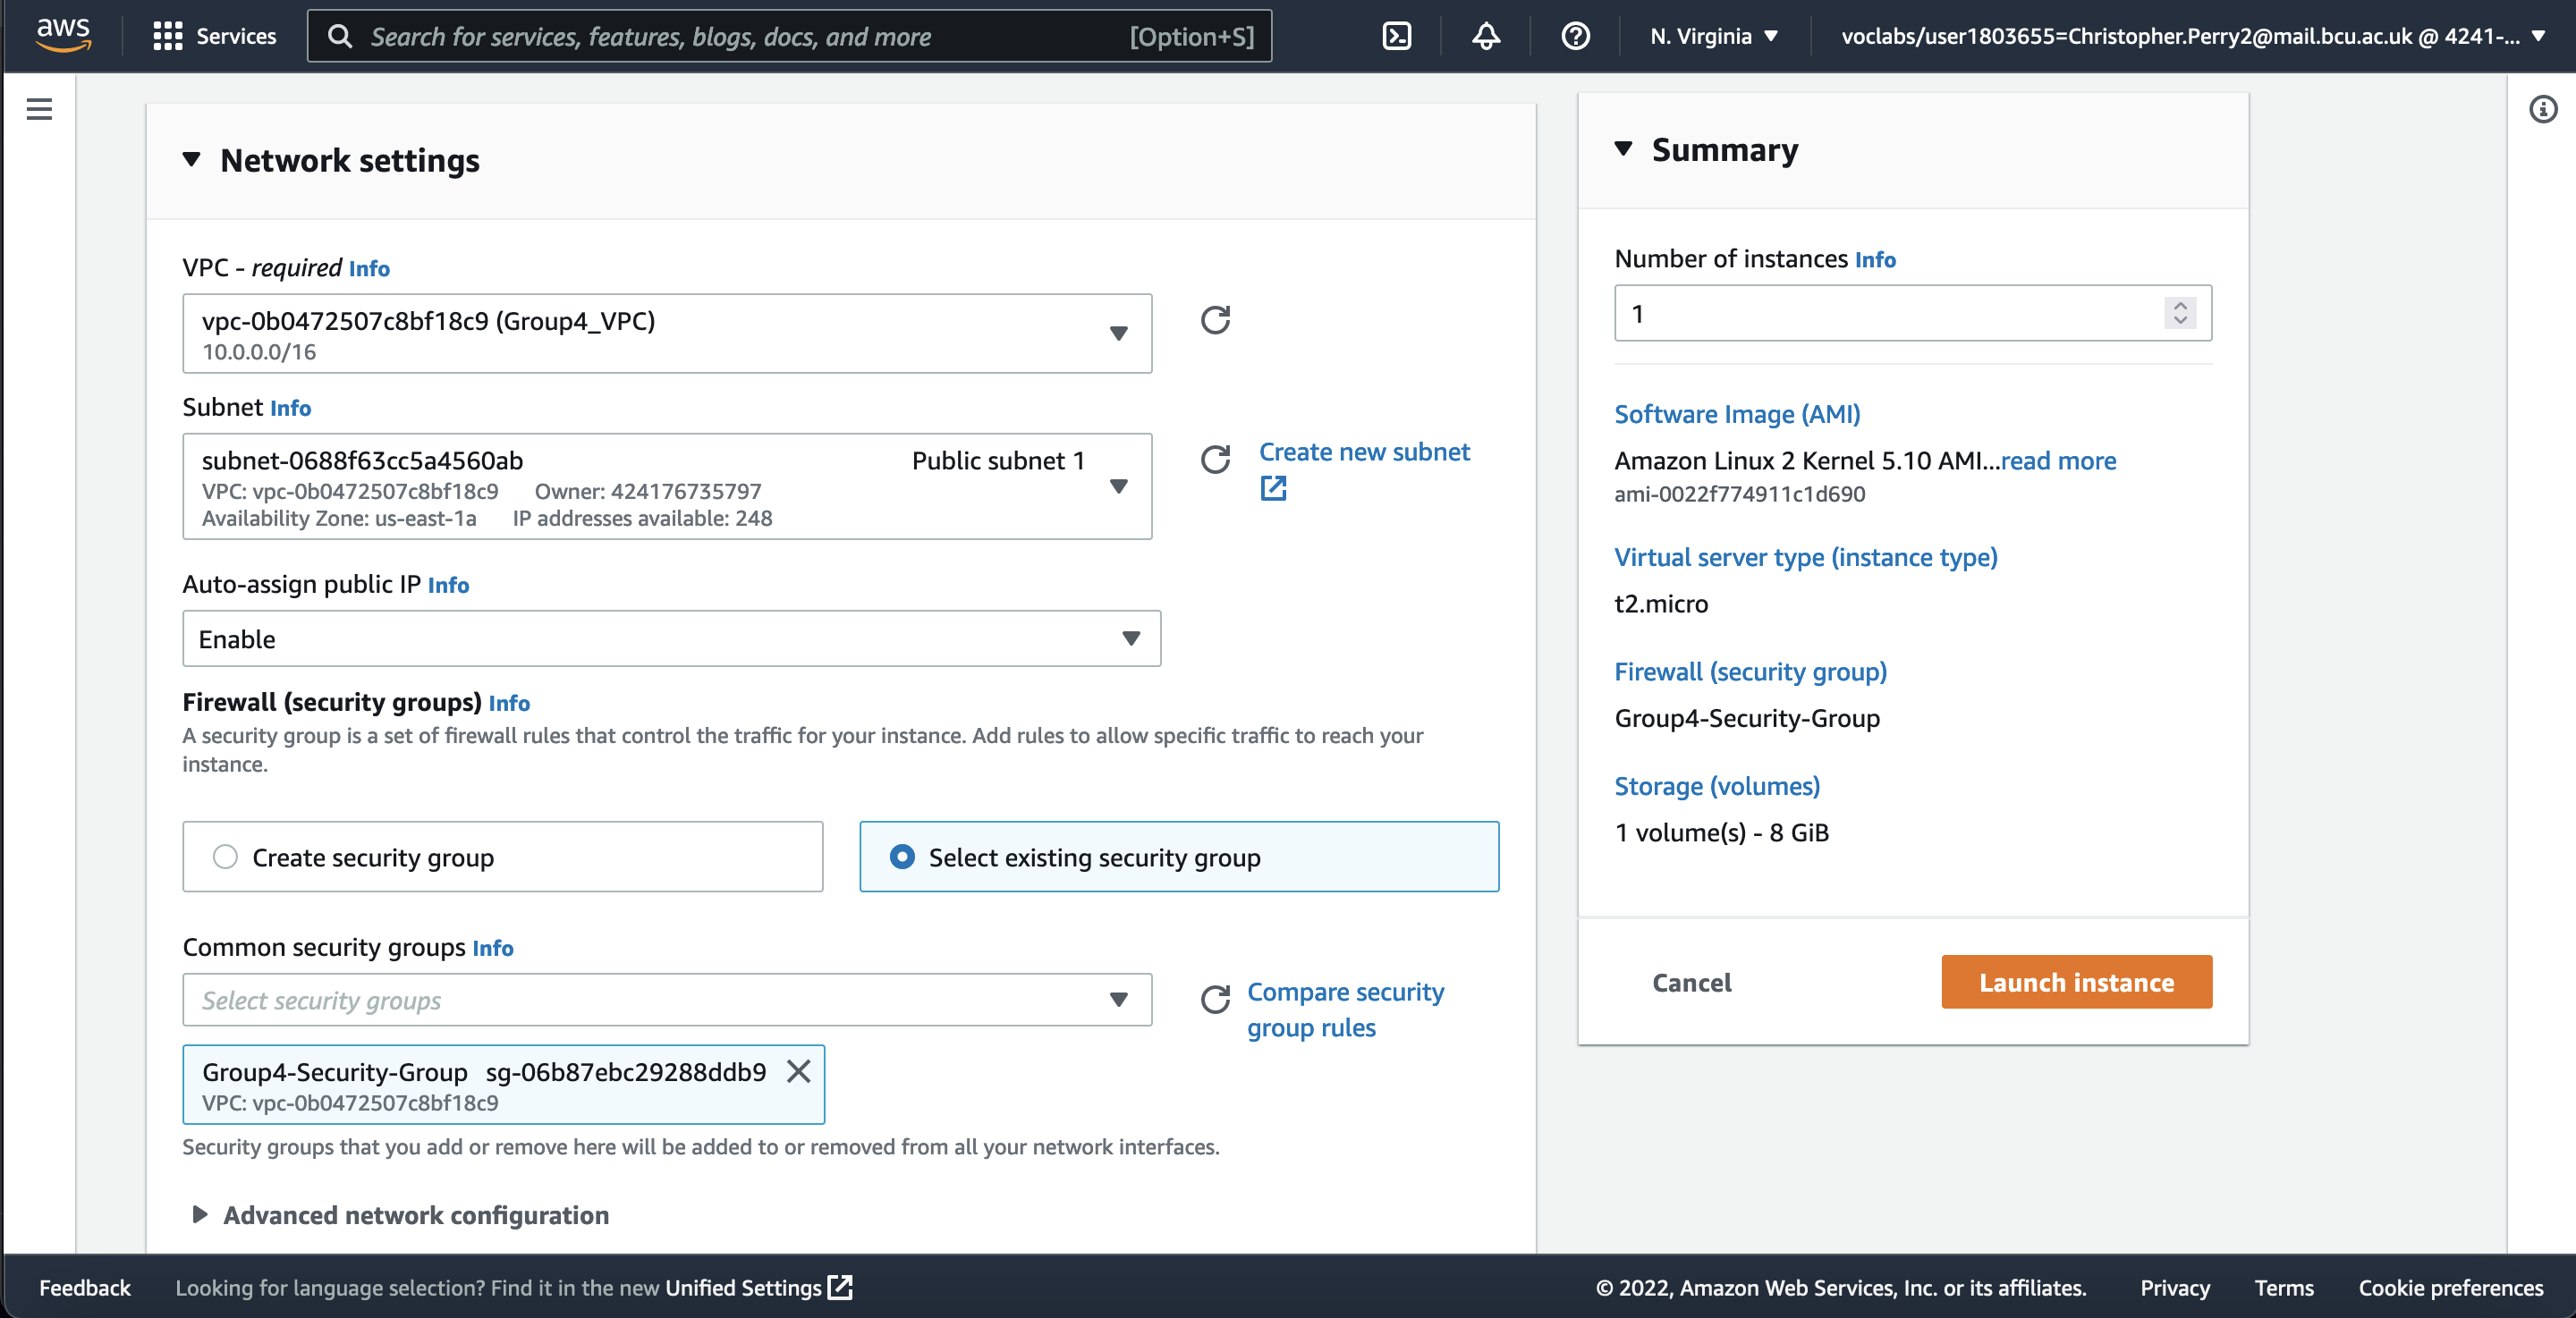
\includegraphics[width=\textwidth]{resources/ec2/create-instance-network-settings}
    \caption{Selection of EC2 Networking options.}
    \label{fig:ec2-networking}
\end{figure}

\begin{figure}[!htbp]
    \centering
    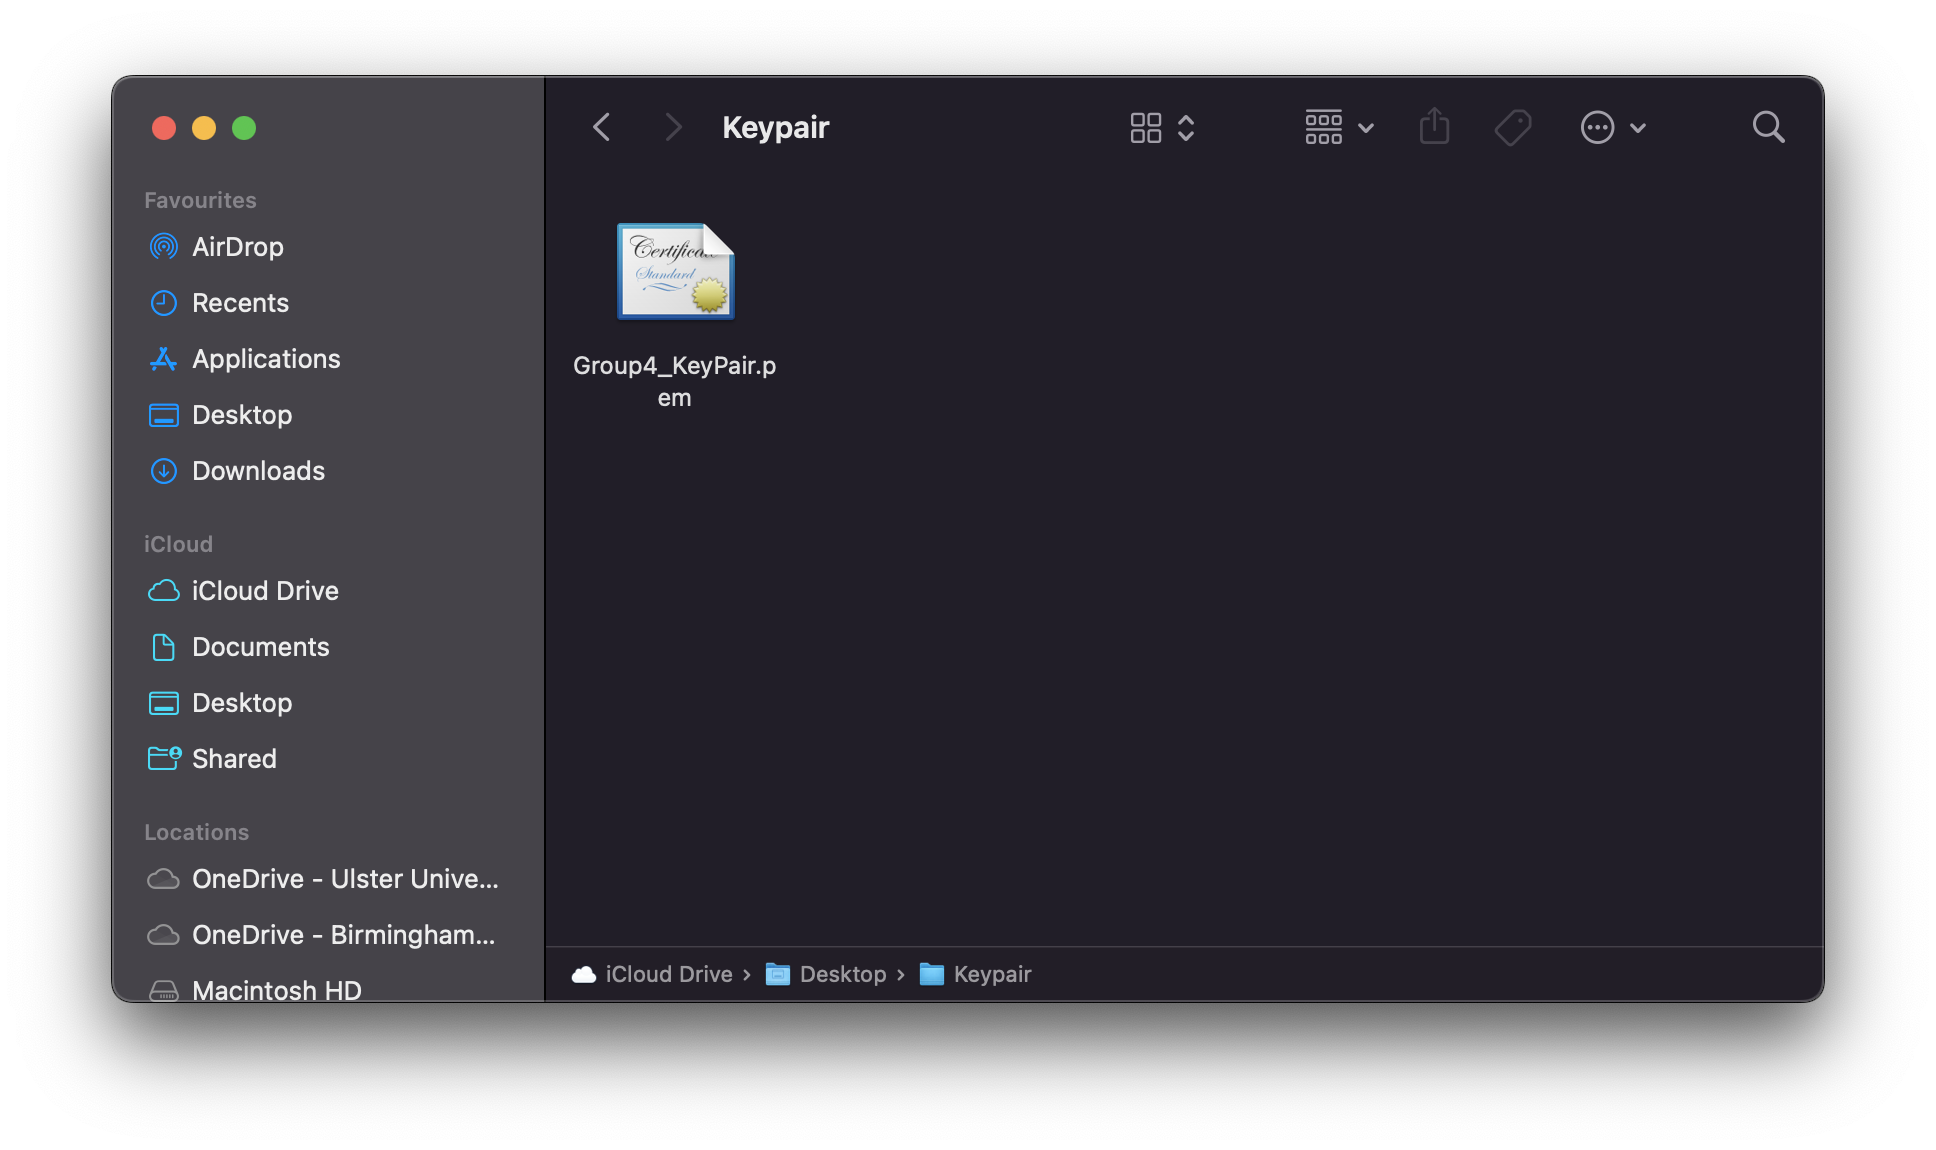
\includegraphics[width=\textwidth]{resources/ec2/keypair}
    \caption{Generated EC2 Keypair in the \mintinline{sql}|.pem| format.}
    \label{fig:keypair}
\end{figure}

This setup can be seen in Figure~\ref{fig:ec2-networking}.
An EC2 keypair is then generated in the \mintinline{sql}|.pem| format.

This is enough to comfortably run the web app without any issues.
Storage for the AMI was subsequently chosen.
It was decided that 8GB of storage would be used, as this is enough to run the web app and still provide leftover
storage for any system-critical tasks.

\begin{figure}[!htbp]
    \centering
    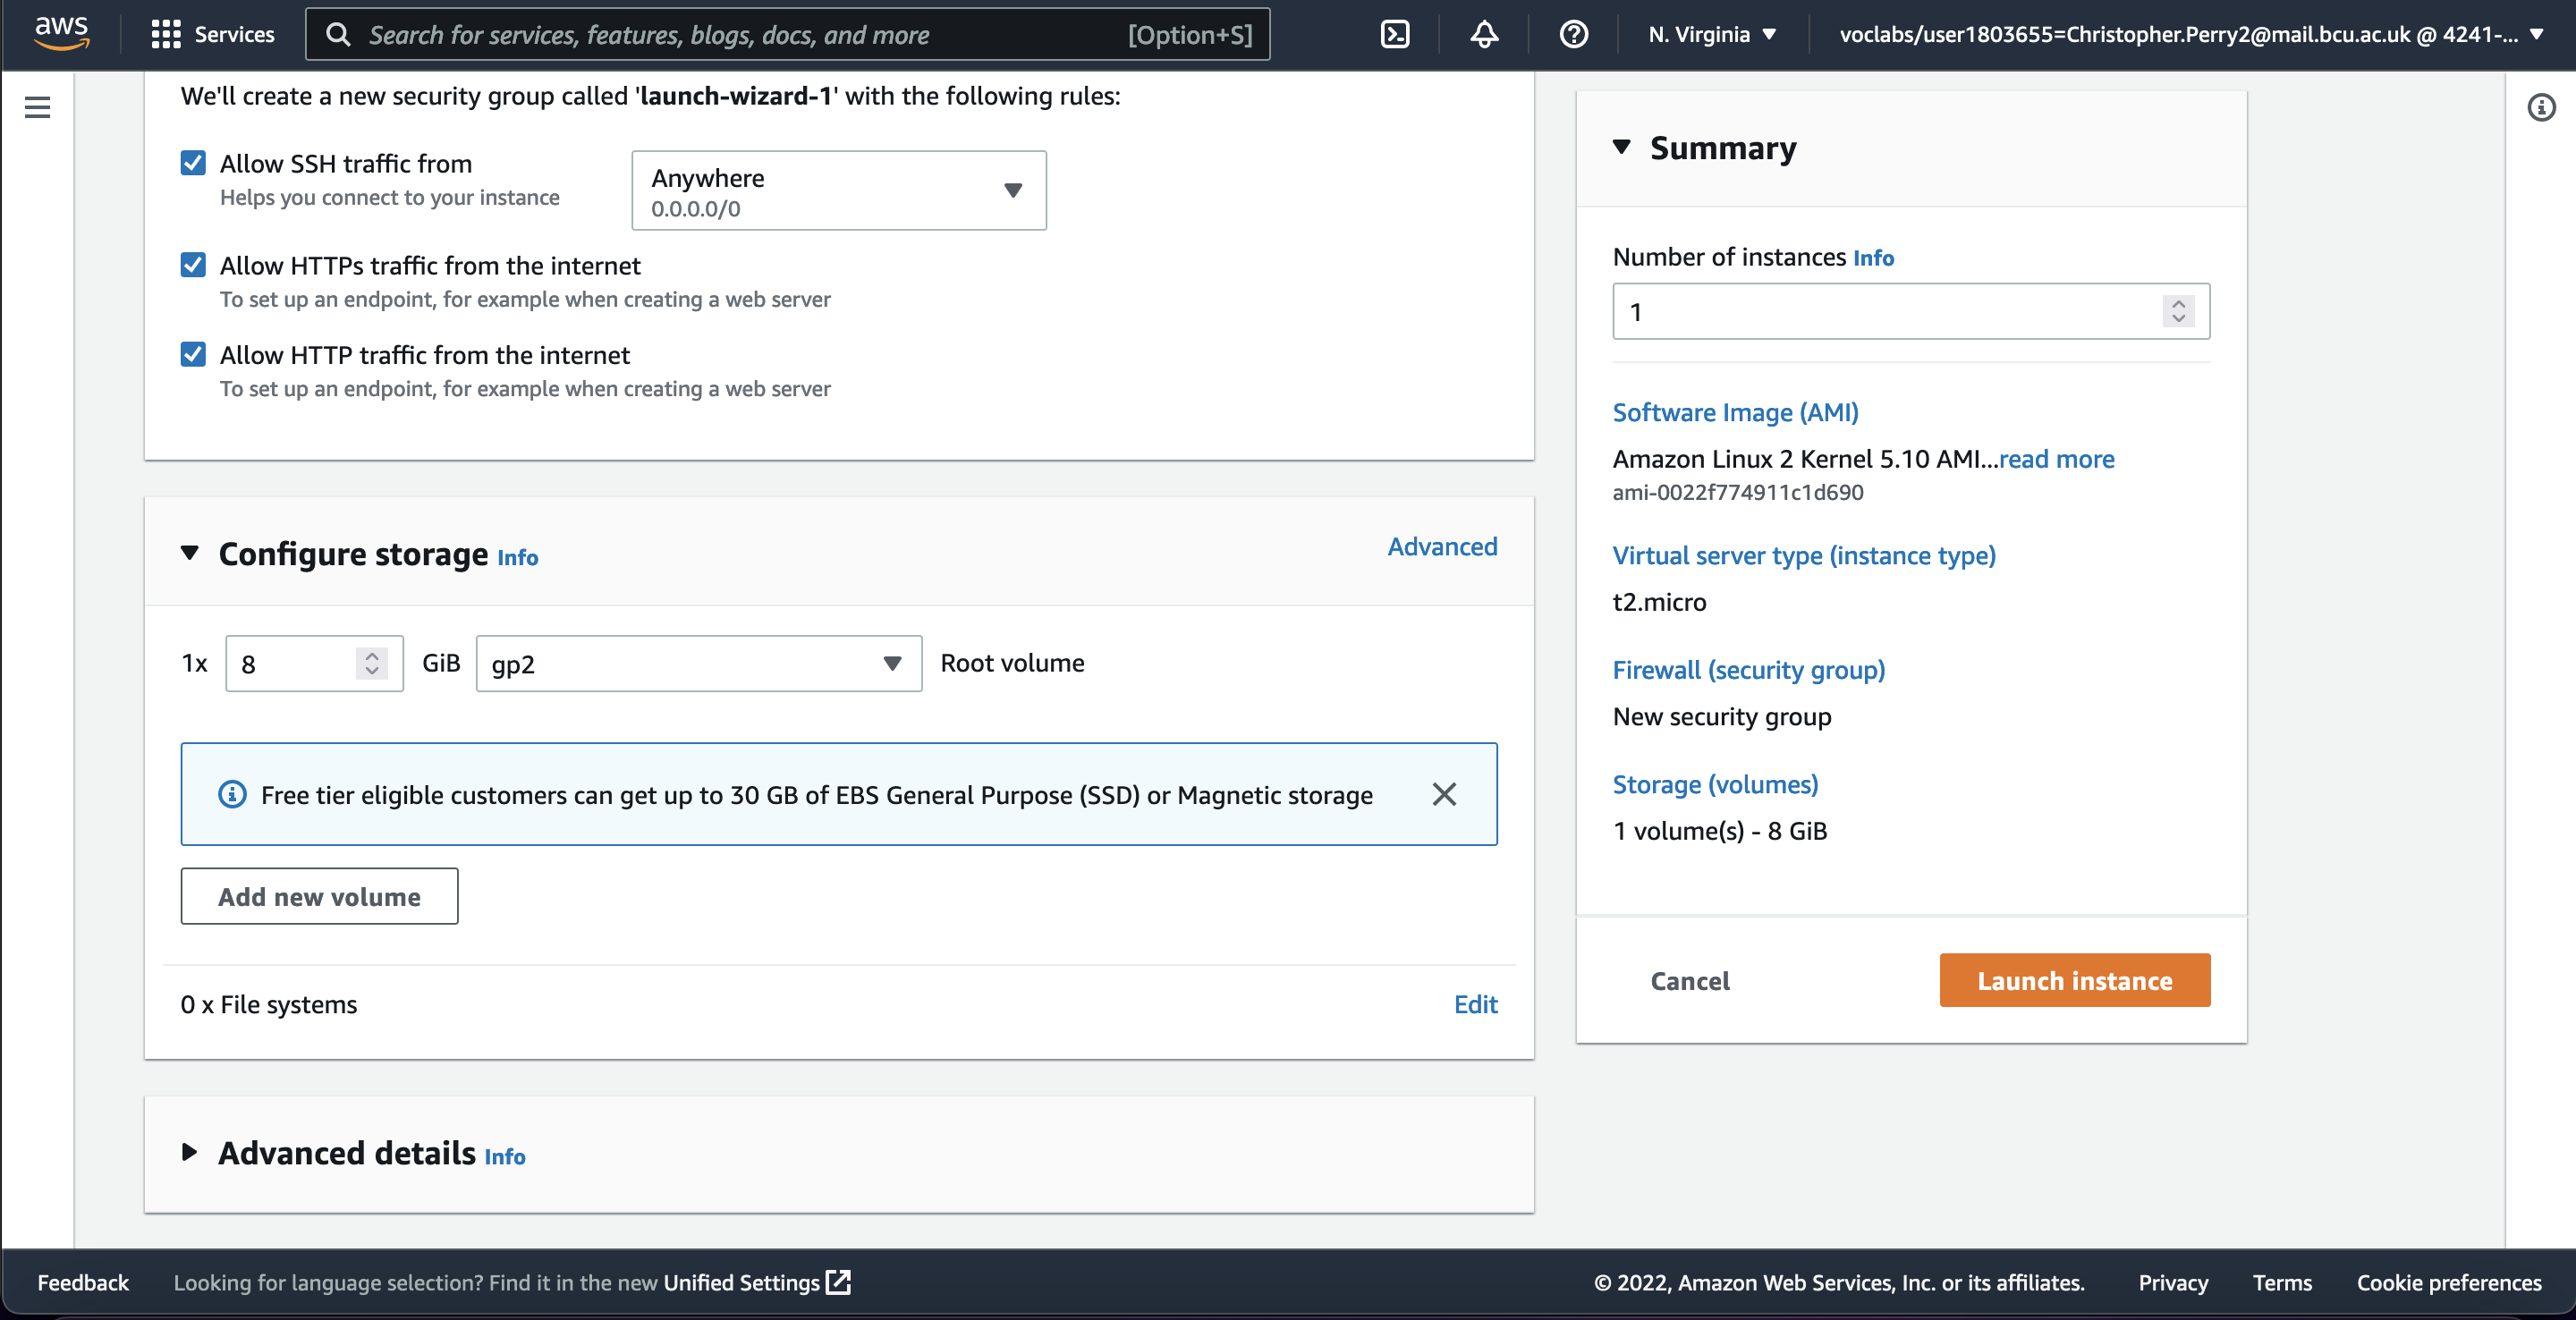
\includegraphics[width=\textwidth]{resources/ec2/create-instance-configure-storage}
    \caption{Selection of EC2 Storage Configuration.}
    \label{fig:ec2-storage}
\end{figure}

The selection of these options can be found in Figure~\ref{fig:ec2-storage}.
In addition to this, the chosen options are eligible for "Free Tier", which means that it will use a limited amount of the
\$100 budget allocated for the project.

\clearpage

\section{EC2 Login}\label{sec:webapp-setup}

The EC2 instance \mintinline{zsh}|group4-ec2| is now live, and the webapp can be loaded onto it.
The instance is first logged in to through the use of the \mintinline{zsh}|ssh| command, followed by the
\mintinline{sql}|-i| argument to specify an identify file, which was generated earlier, and then the public ipv4 address
of the instance.

\begin{figure}[!htbp]
    \centering
    \begin{minted}{zsh}
ssh -i ~/Desktop/Group4_KeyPair.pem ec2-user@52.45.13.111
    \end{minted}
    \caption{SSH command to log into EC2 instance.}\label{fig:ssh-login}
\end{figure}

This command can seen being executed in Figure~\ref{fig:ssh-login}.

\begin{figure}[!htbp]
    \centering
    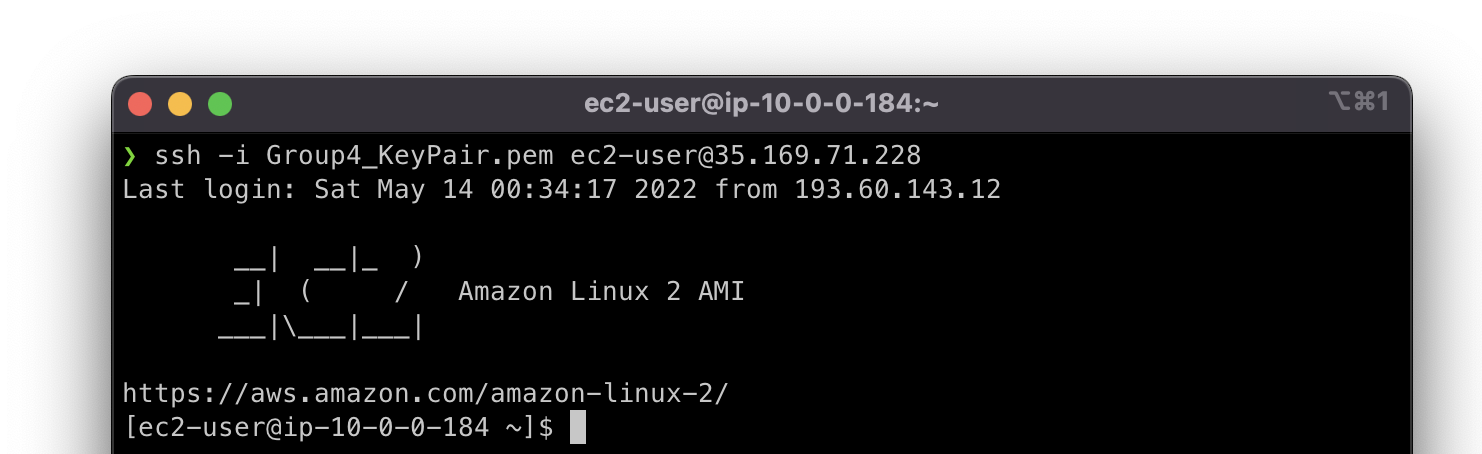
\includegraphics[width=\textwidth]{resources/ec2/ec2-logged-in}
    \caption{Logging into EC2 instance.}
    \label{fig:ec2-logged-in}
\end{figure}

The logged in EC2 instance can be seen in Figure~\ref{fig:ec2-logged-in}.

\clearpage
\section{Package Setup}\label{sec:web-app-setup}

The web app is stored on GitHub, and the AMI does not come with GitHub by default.
Git is subsequently installed via \mintinline{zsh}|yum install git|.

\begin{figure}[!htbp]
    \centering
    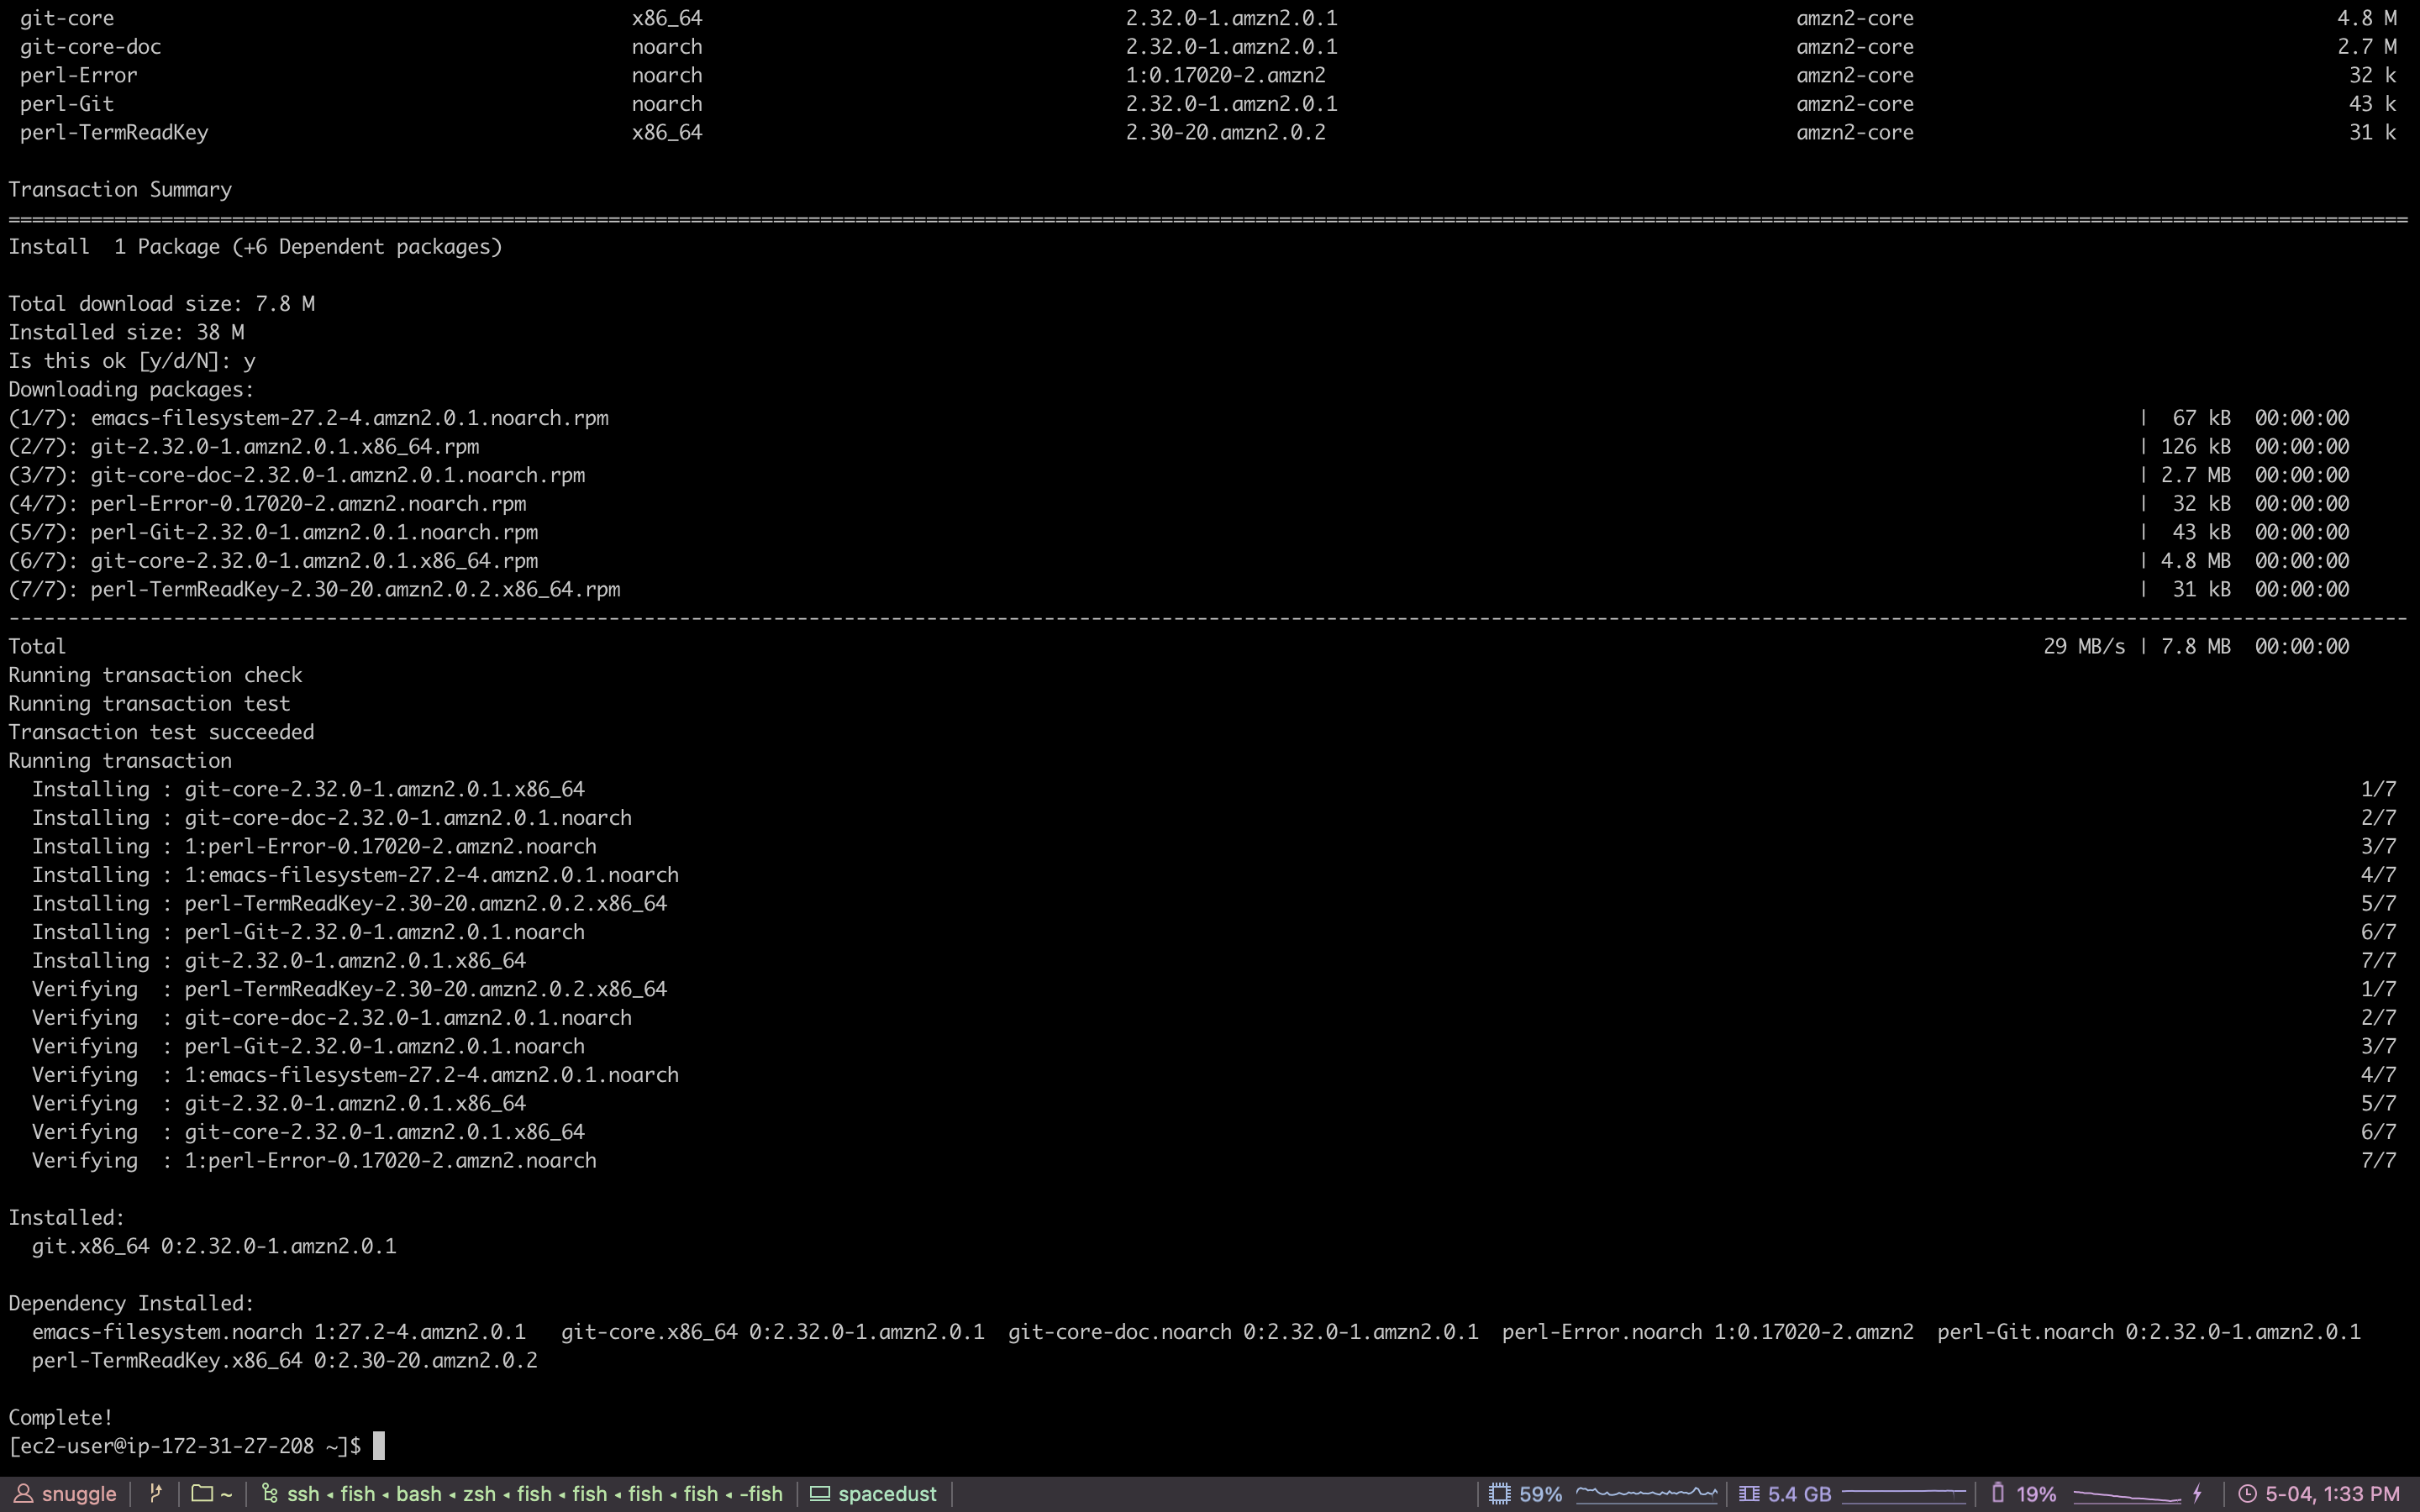
\includegraphics[width=\textwidth]{resources/ec2/installing-git}
    \caption{Installing Git.}
    \label{fig:webapp-git}
\end{figure}

The web app also requires docker, and \mintinline{zsh}|yum install docker| is executed to install Docker as a result.

\clearpage

\begin{figure}[!htbp]
    \centering
    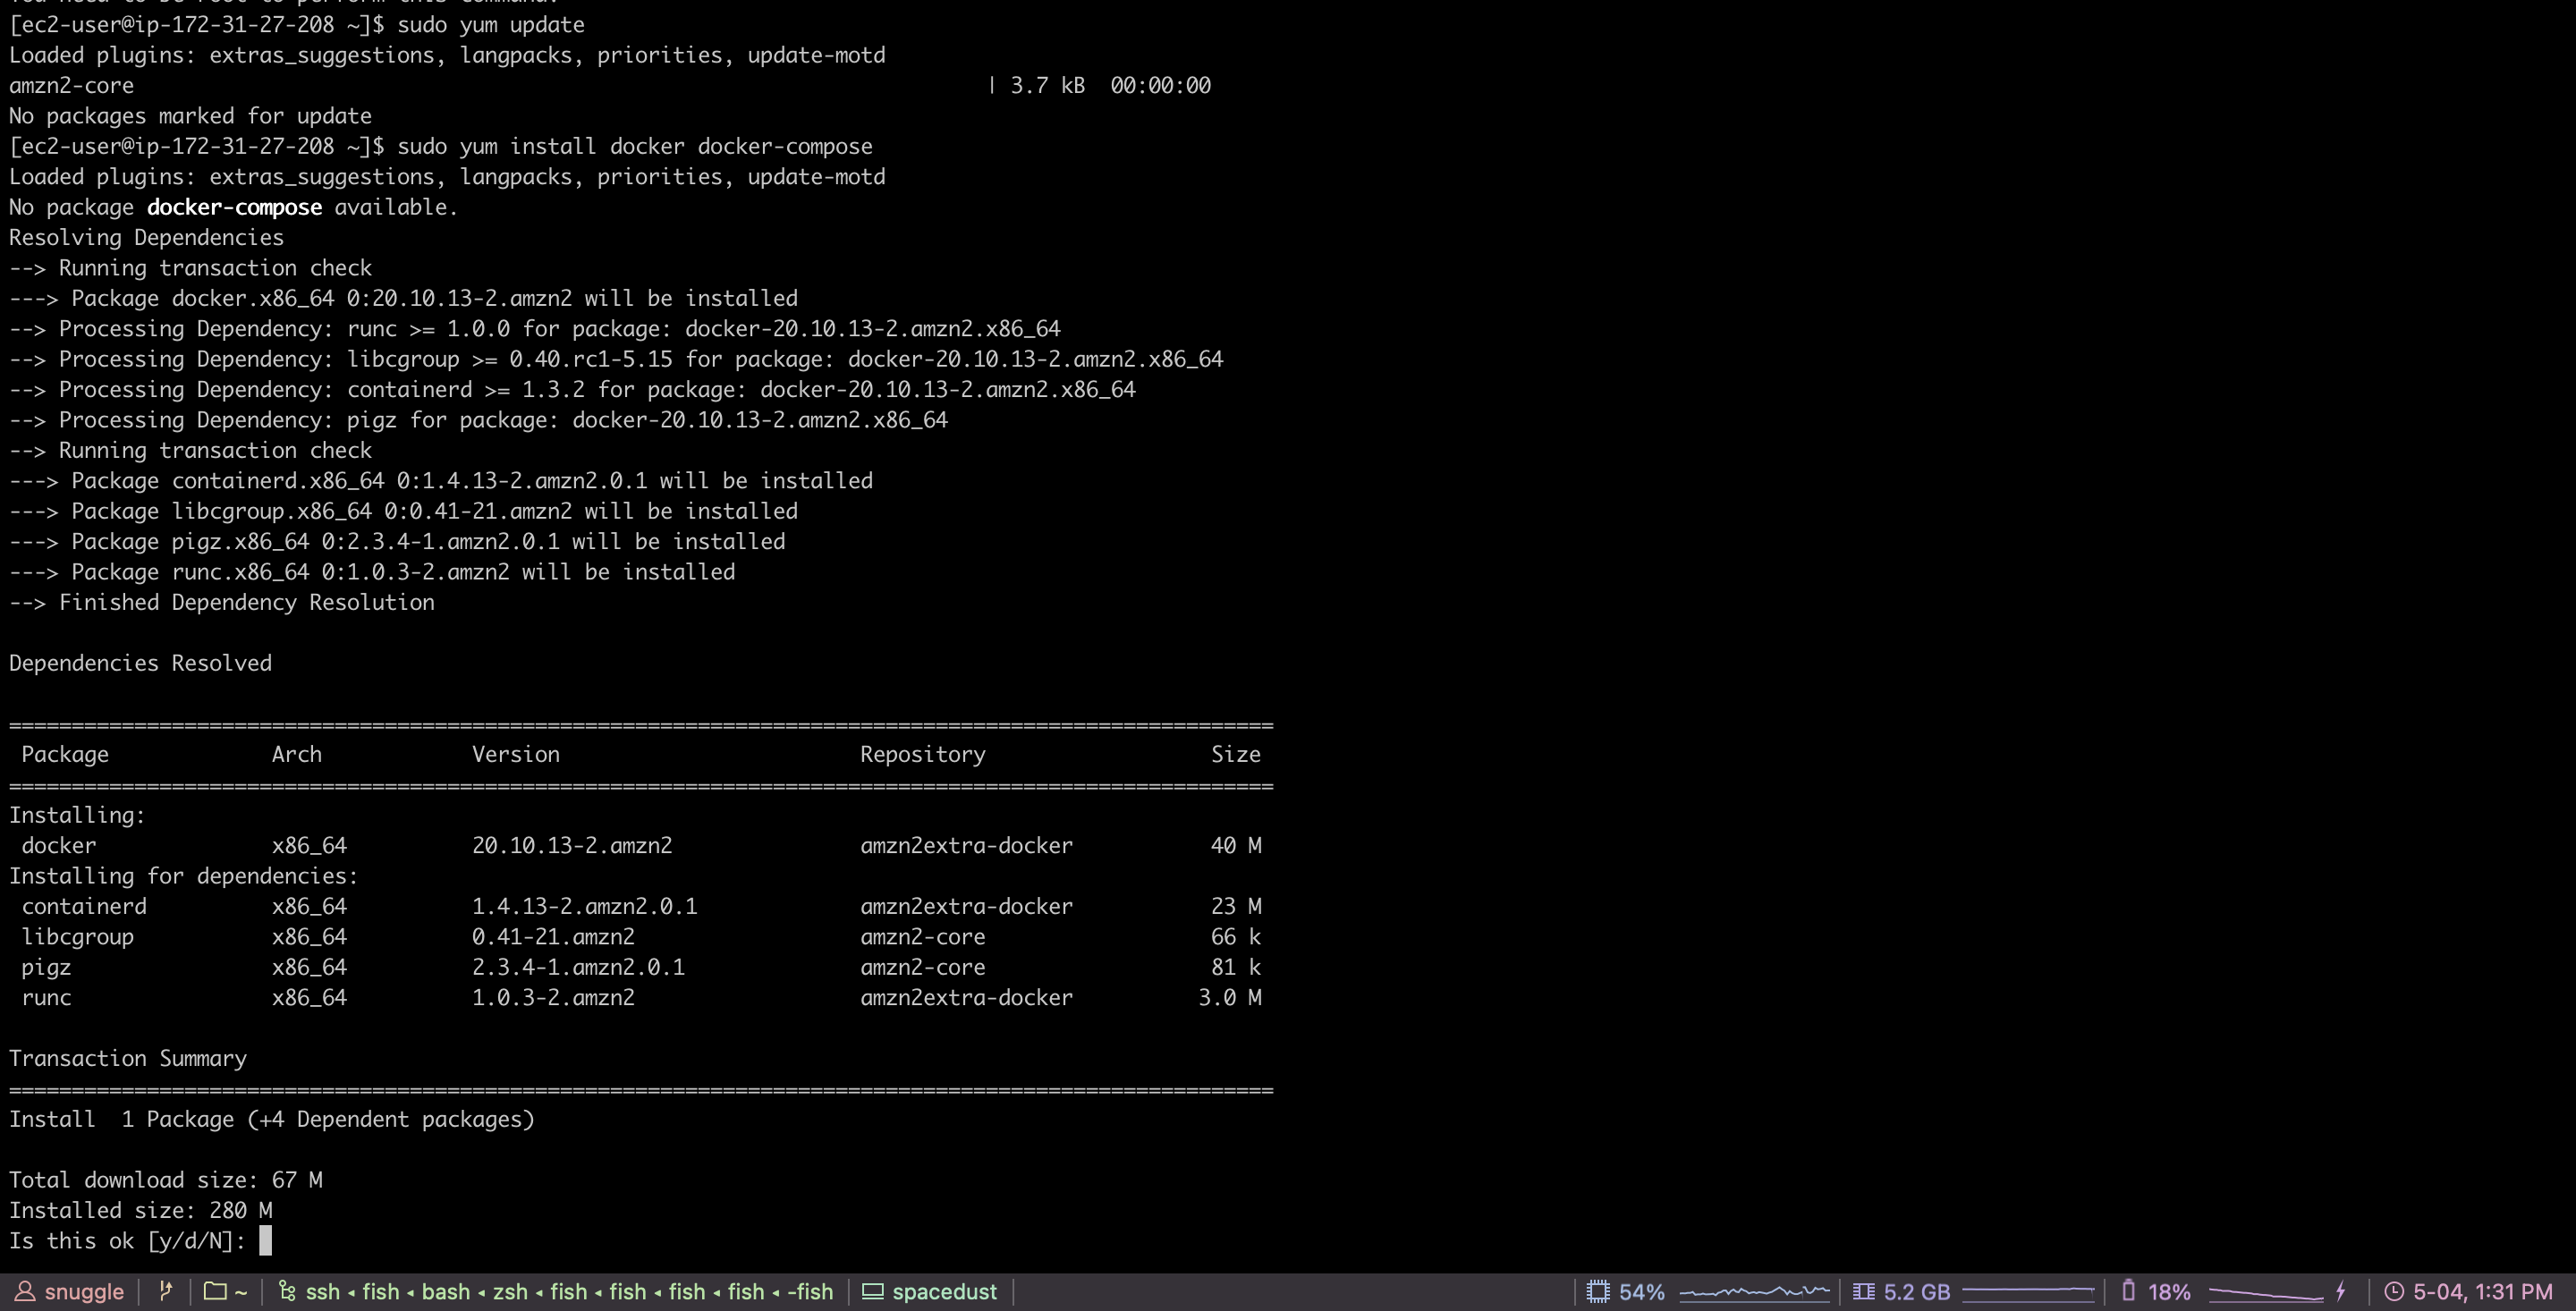
\includegraphics[width=\textwidth]{resources/ec2/installing-docker}
    \caption{Installing Docker.}
    \label{fig:webapp-docker}
\end{figure}

\section{Web App Setup}\label{sec:web-app-setup2}

The web app is firstly cloned from its repository via the \mintinline{zsh}|git clone| command, and a new
\mintinline{zsh}|digital-ink| folder is made to store the contents.

\begin{figure}[!htbp]
    \centering
    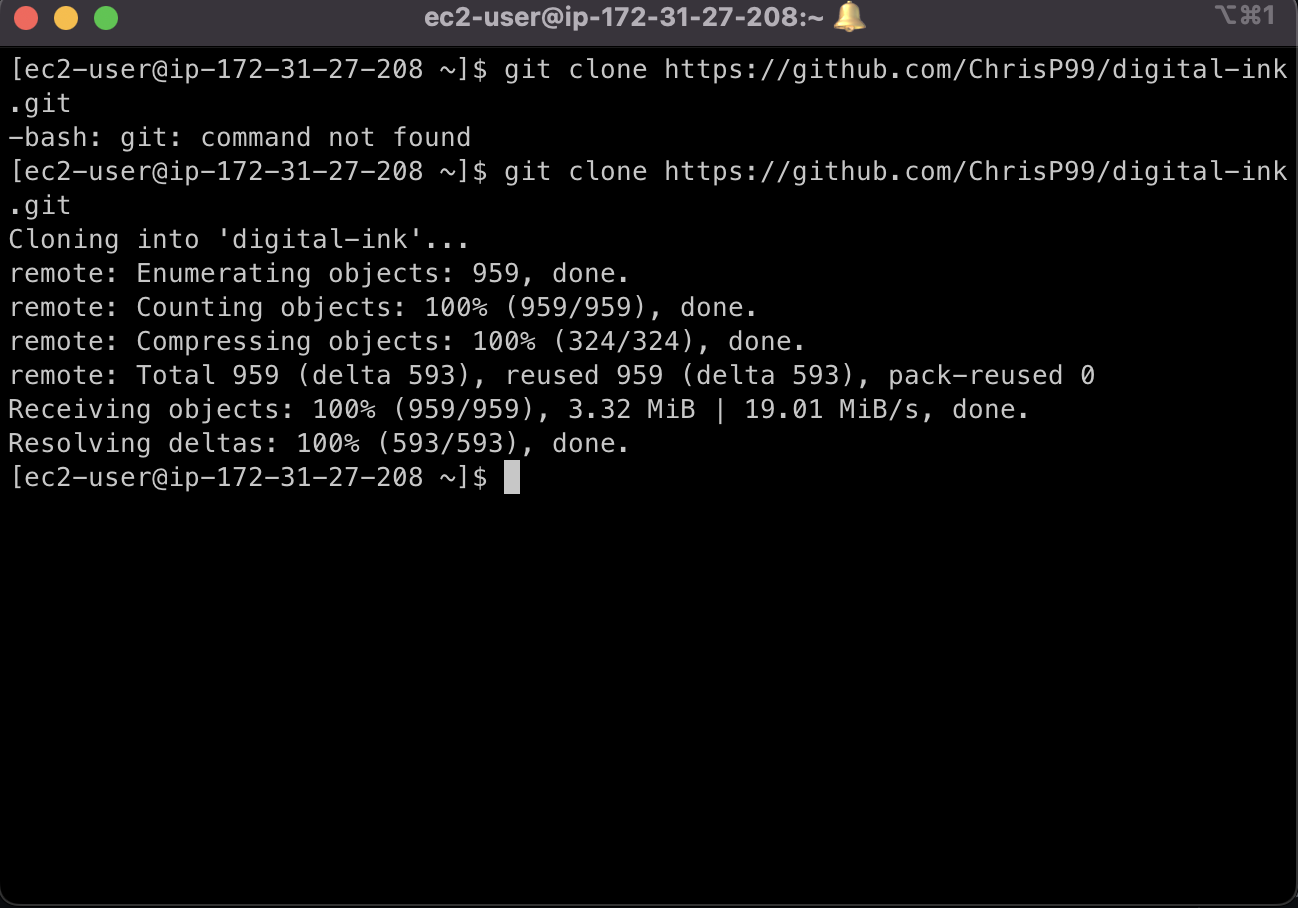
\includegraphics[width=\textwidth]{resources/ec2/webapp-clone}
    \caption{Cloning the web app from Github.}
    \label{fig:webapp-clone}
\end{figure}

The \mintinline{zsh}|cd| command is used to move into the \mintinline{zsh}|digital-ink| folder, and the web app is
subsequently launched through the \mintinline{docker}|docker-compose up -d| to launch the web app as a detached Docker
container.
Relevant containers that are required to be downloaded from the \mintinline{docker}|dockerfile| are then pulled.

\begin{figure}[!htbp]
    \centering
    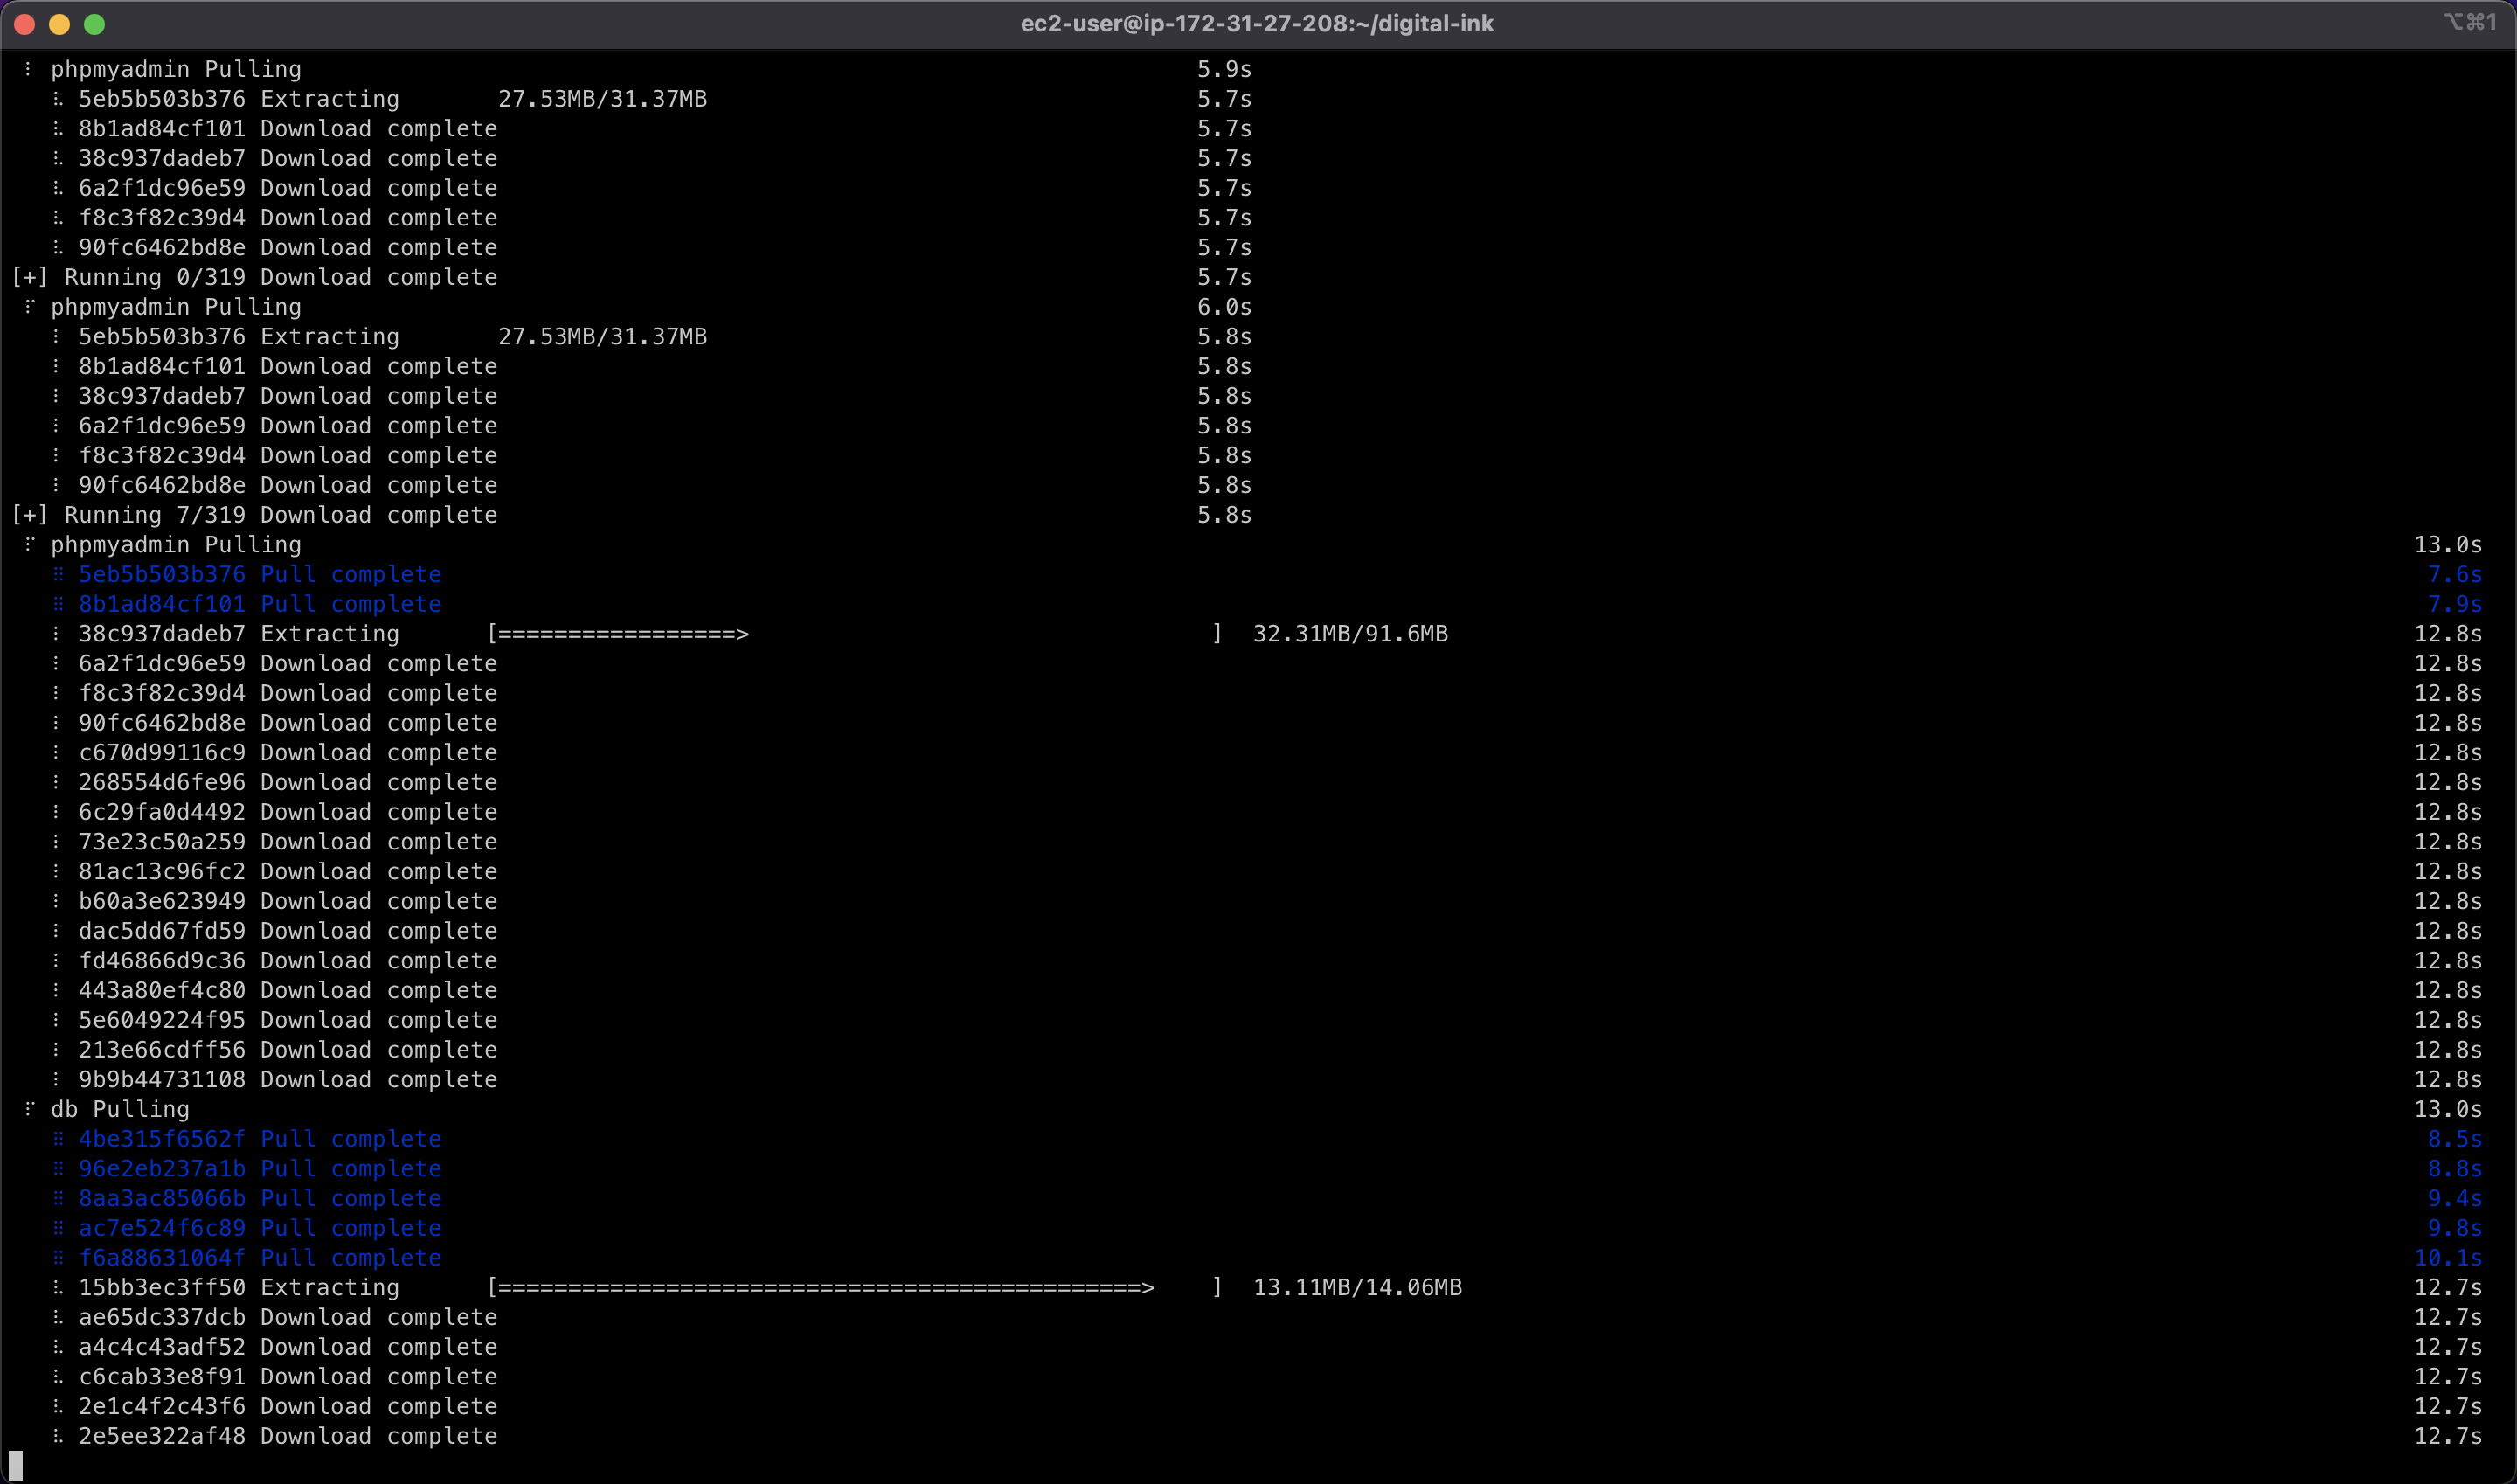
\includegraphics[width=\textwidth]{resources/ec2/docker-compose}
    \caption{Containers required for the web app being pulled from Docker Hub.}
    \label{fig:webapp-docker-compose}
\end{figure}

The result of this command launches 3 containers:

\begin{enumerate}
    \item \mintinline{docker}|digital-ink|: An instance of the web app which uses a custom Laravel container.
    \item \mintinline{docker}|mysql|: An instance of a local database made in MySQL\@.
    \item \mintinline{docker}|phpmyadmin|: A way to locally manage the database through a UI\@.
\end{enumerate}

At the minute, the web app is live through the \mintinline{docker}|digital-ink| container, and is using a local version
of MySQL as a database, stored within the \mintinline{docker}|mysql|Docker container.
The database has no tables, but can be populated through the use of Laravel.
The container is firstly accessed through \mintinline{docker}|docker exec app bash|, and the database is populated with
tables with \mintinline{zsh}|php artisan migrate|.
This then generates tables to store users and their stories.

\begin{figure}[!htbp]
    \centering
    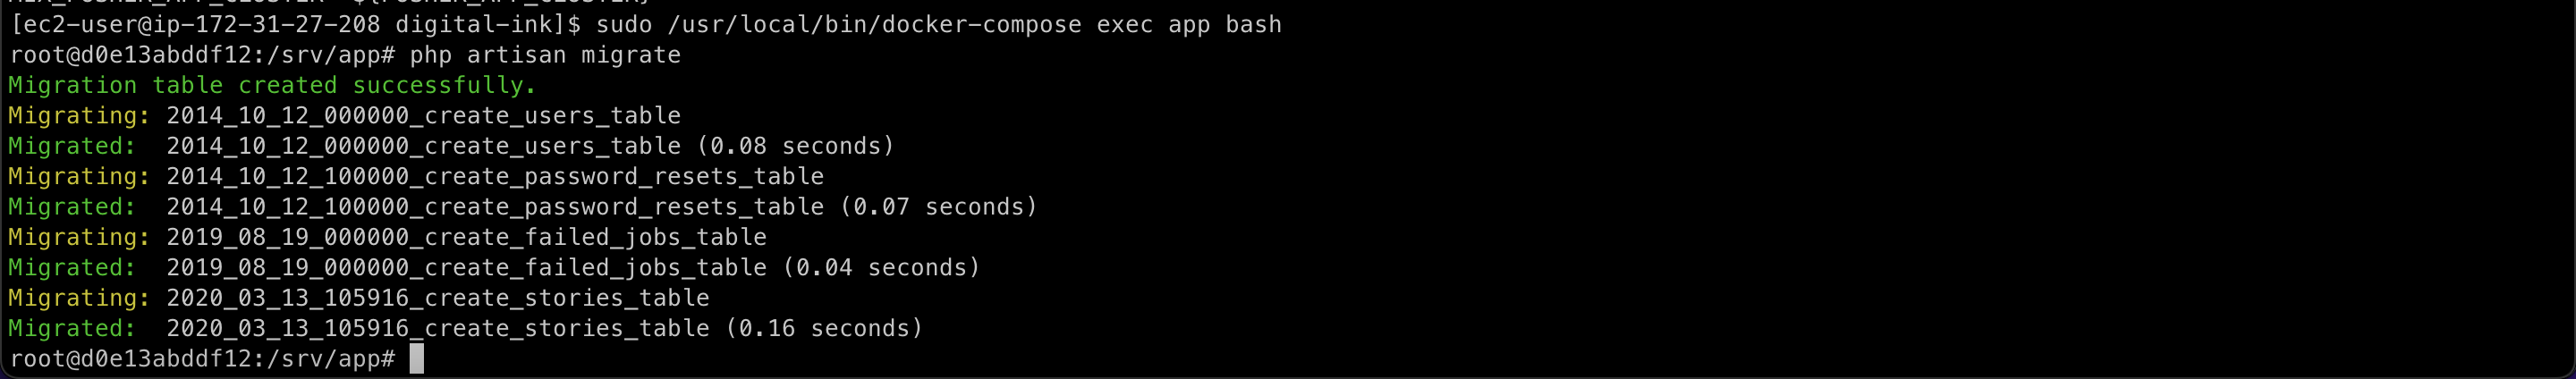
\includegraphics[width=\textwidth]{resources/ec2/php-artisan-migrate}
    \caption{Creation of tables through \mintinline{zsh}|php artisan migrate| command. }
    \label{fig:php-artisan-migrate}
\end{figure}

The subsequent output of this command can be found in Figure~\ref{fig:php-artisan-migrate}
















    % Evie Lives here
\section{systemd Services}
systemd is a service manager, which is a program that launches and monitors different services across the system. The digital-ink application is automatiacally started upon boot by the systemd process, which ensures that the application is started correctly and without errors. If any errors occur, systemd will log them in a tool known as journalctl and then follow a configuration file for instructions on how to handle those errors. This can range from simply restarting a program that has errored, to trying once again, or recording the failure and performing no action.

\begin{figure}
    \centering
    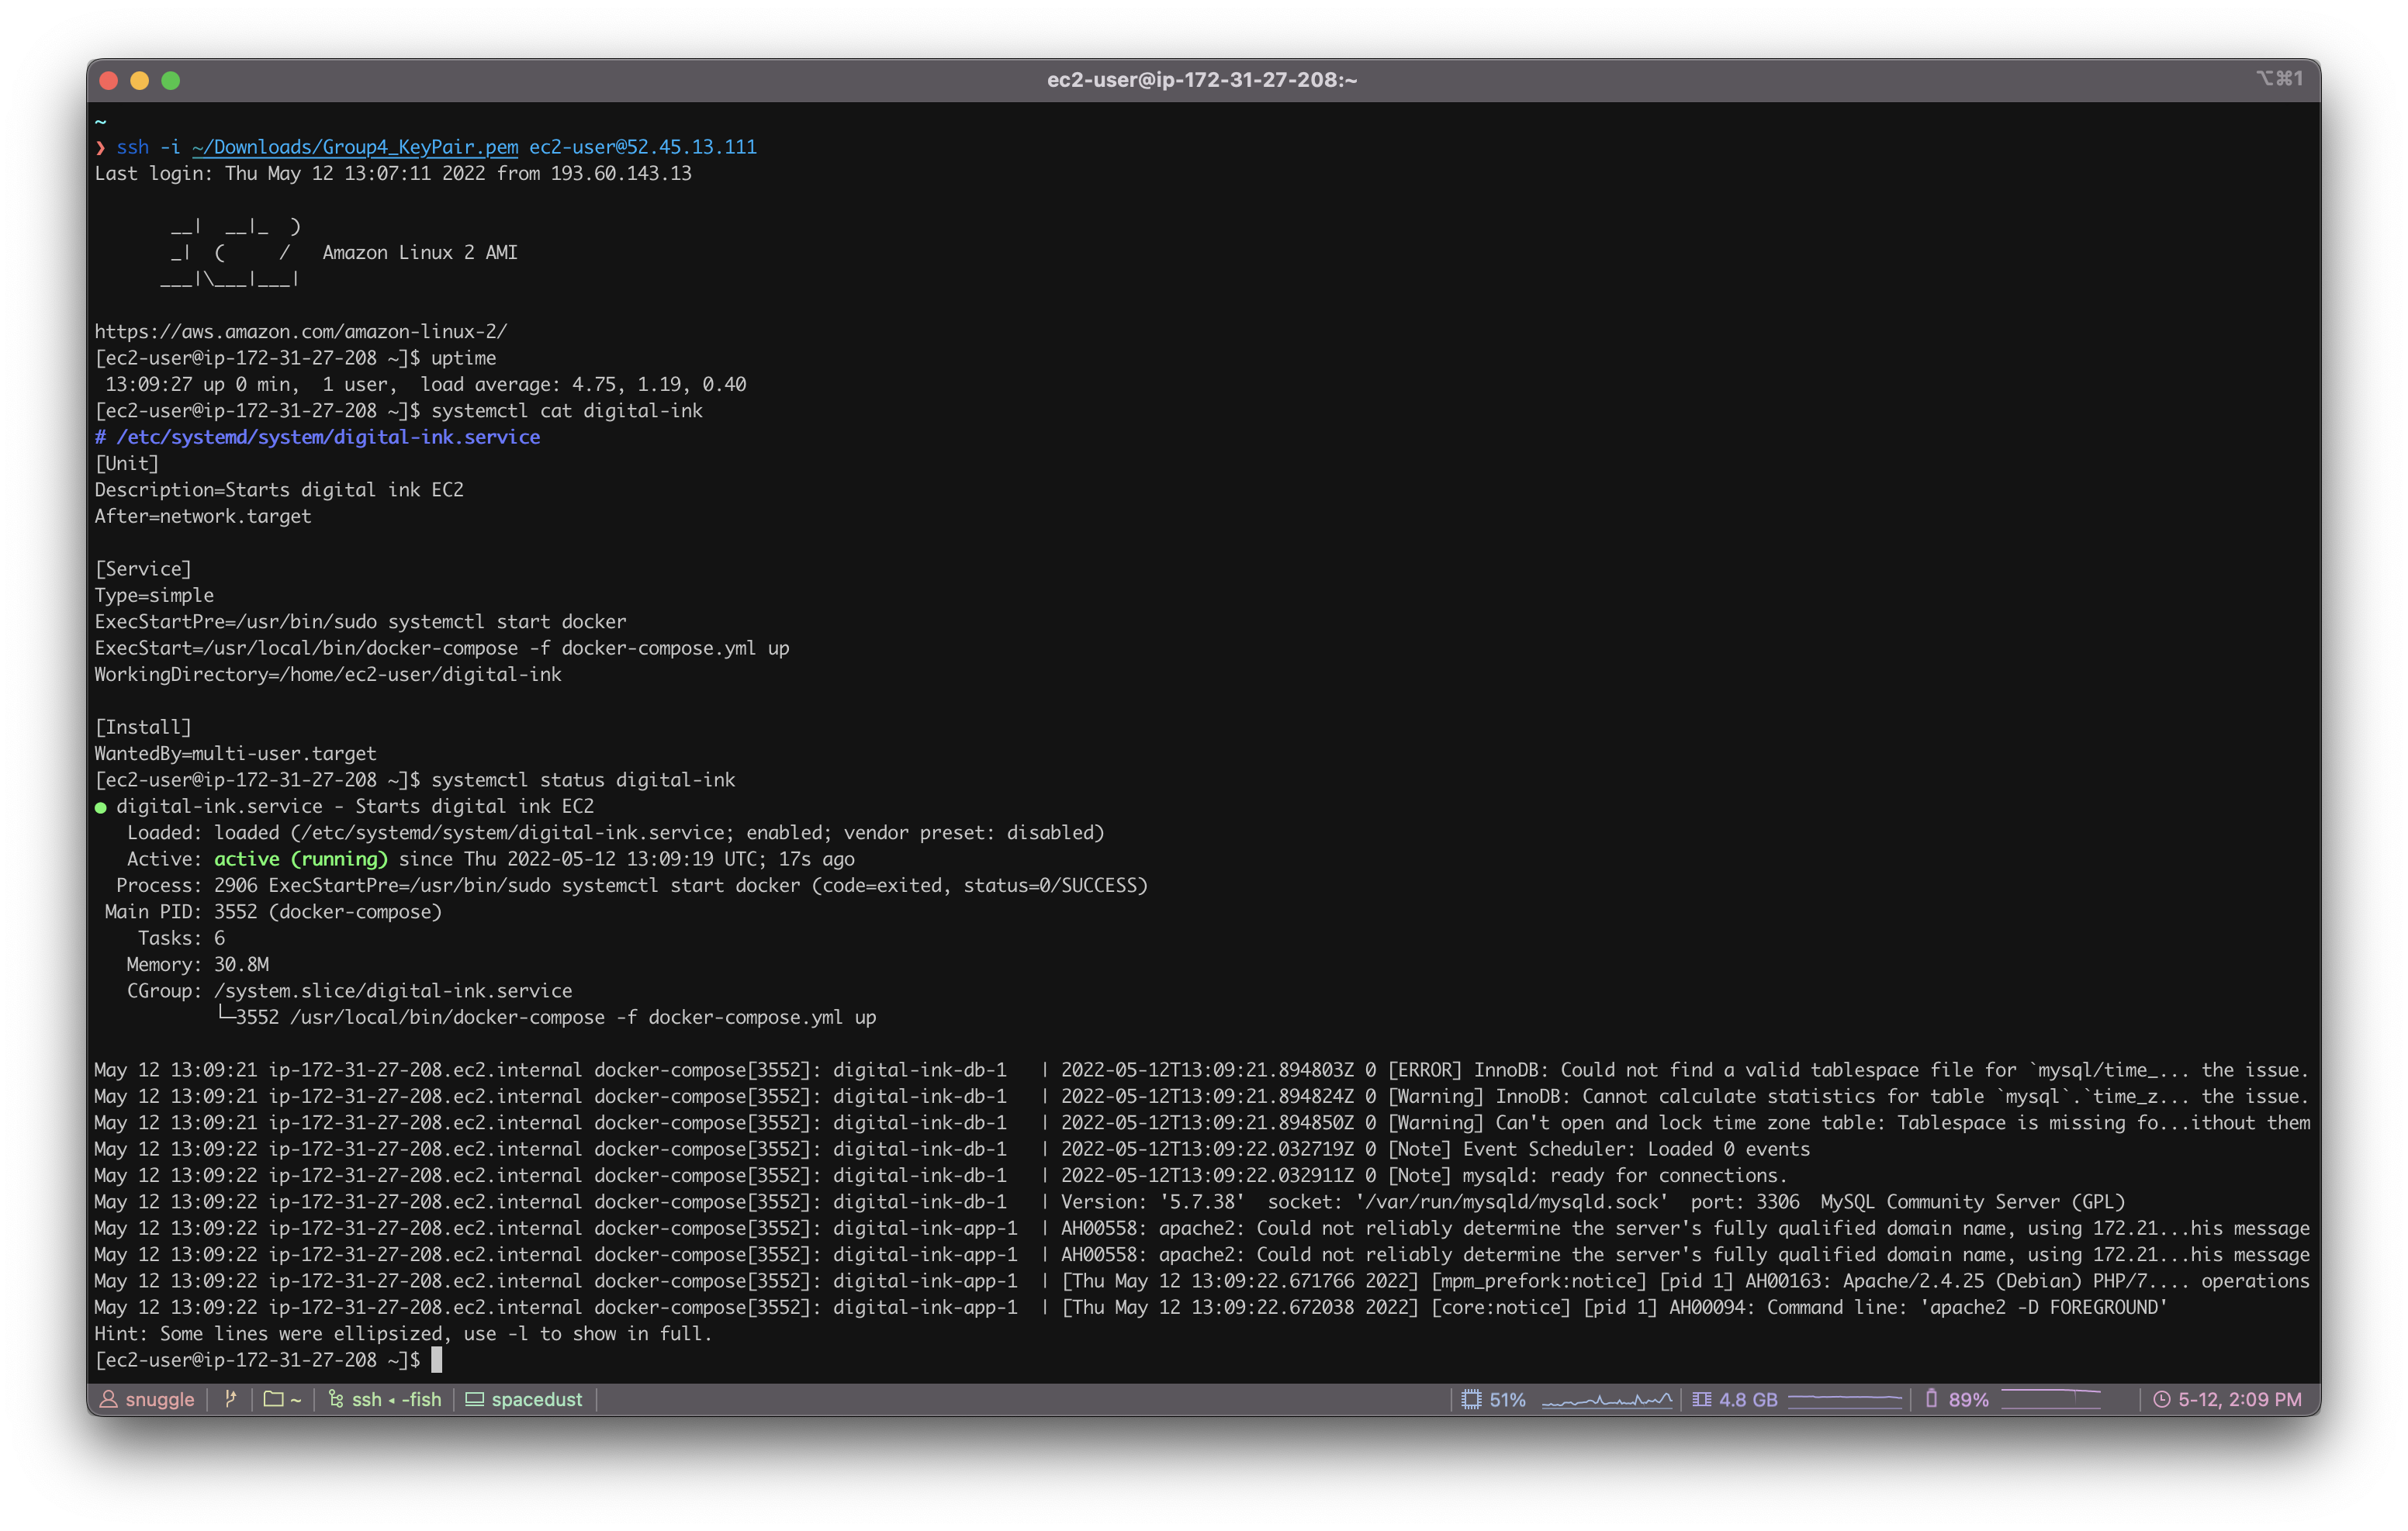
\includegraphics[width=\textwidth]{resources/systemd/systemd.png}
    \caption{Creation of systemd Service}
    \label{fig:systemd}
\end{figure}

    \chapter{Simple Storage Service (S3)}\label{ch:simple-storage-service}

\section{What is Simple Storage Service (S3)?}
AWS S3 is a form of cloud-based object storage.
This is a style of network filesystem that treats each file as a separate object with a unique ID, which allows each
object to be served individually over a network with a single URL, which can also be enhanced with a content delivery
network~\parencite{amazon2022cloud}.

Each S3 instance is seperated into logical containers known as buckets.
Each S3 bucket can have its own credentials, its own endpoint and other permissions and configuration.
Object storage is particularly useful when creating an application that scales as you are billed per unit of storage
that you use, and in theory are able to use infinite storage as your application demands.
The only limitation with object storage is how much you are able to pay for.
Each object is automatically replicated across many nodes, providing data redundancy against multiple different
availability zones.

S3 is perhaps the most popular AWS service and used by many SaaS applications across the internet, for instance
Instagram, Facebook, Discord and Twitter are all known for using S3 or S3-style storage.
The advent of object storage has created an almost de-facto standard, which has lead for the creation of many
'S3-compatible' or 'S3-like' competitor solutions, such as those run by Google Cloud and Microsoft Azure.

\section{Creating an S3 Bucket}

\subsection{TODO}

\begin{figure}
    \centering
    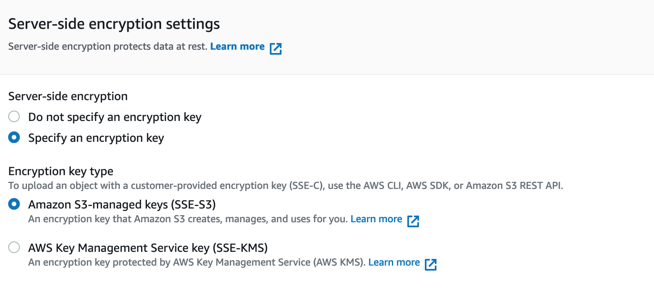
\includegraphics[width=\textwidth]{resources/s3/s3_encryption.PNG}
    \caption{Setting up S3 Encryption Key}
    \label{fig:s3-image-2}
\end{figure}

\section{Using S3 URLs within Code}

\subsection{TODO}

TODO

\section{Testing S3 Working}

\begin{figure}
    \centering
    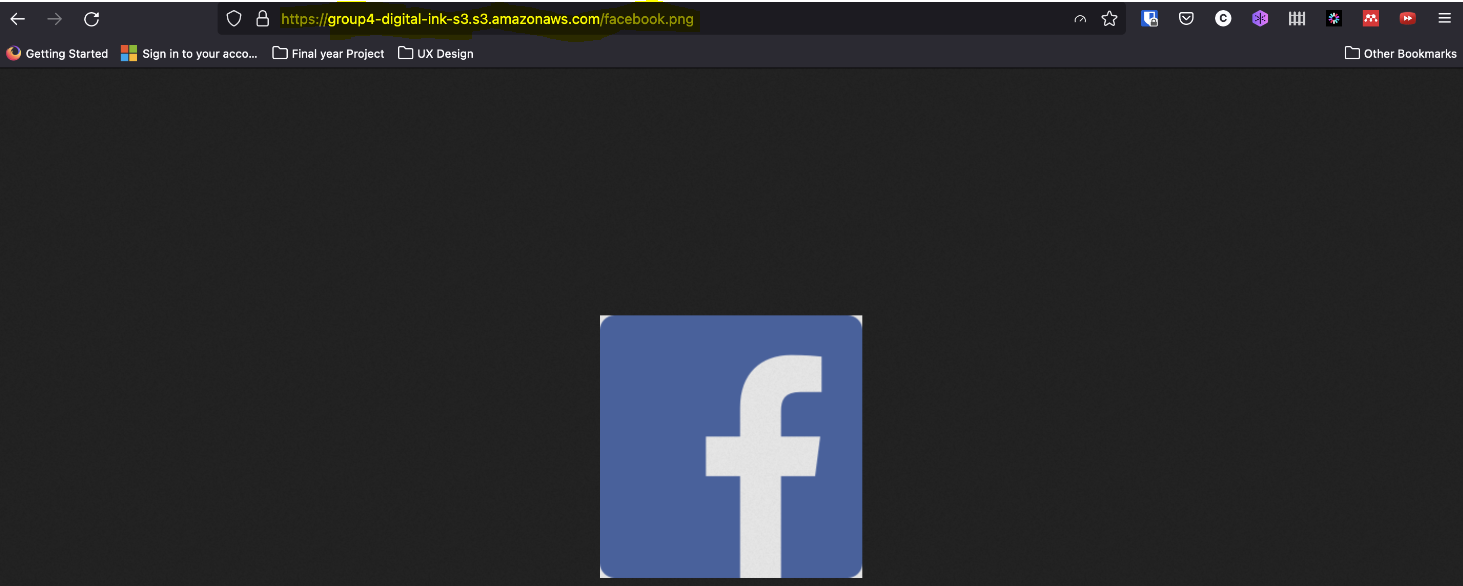
\includegraphics[width=\textwidth]{resources/s3/s3-image-displayed}
    \caption{Image access through S3}
    \label{fig:s3-image}
\end{figure}


\section{Content Distribution Network (CDN)}
Please see Chapter~\ref{ch:cloudfront}.


    \chapter{CloudFront}\label{ch:cloudfront}

CloudFront will allow for the distribution of static and dynamic web images more efficiently.
An international network of data centres, referred to as edge locations, are used to deliver content for CloudFront.
An edge location which offers the lowest latency or delay in serving these files will be used.
This will involve the creation of a CloudFront Distribution.

Firstly, an origin is chosen which is the S3 bucket created in Section~\ref{ch:simple-storage-service}.
It is then given a name of \mintinline{zsh}|group4-digital-ink.s3.us-east-1.amazonaws.com|.
The "Yes use OAI" option is selected, in order to restrict bucket access to only CloudFront.
The "Bucket Policy" option is set to "Yes" to automatically update permissions on the bucket to allow read access for
the OAI.
These options can be seen configured in Figures~\ref{fig:cloudfront-bucket-policy} and~\ref{fig:cloudfront-origins}.

\clearpage

\begin{figure}[!htbp]
    \centering
    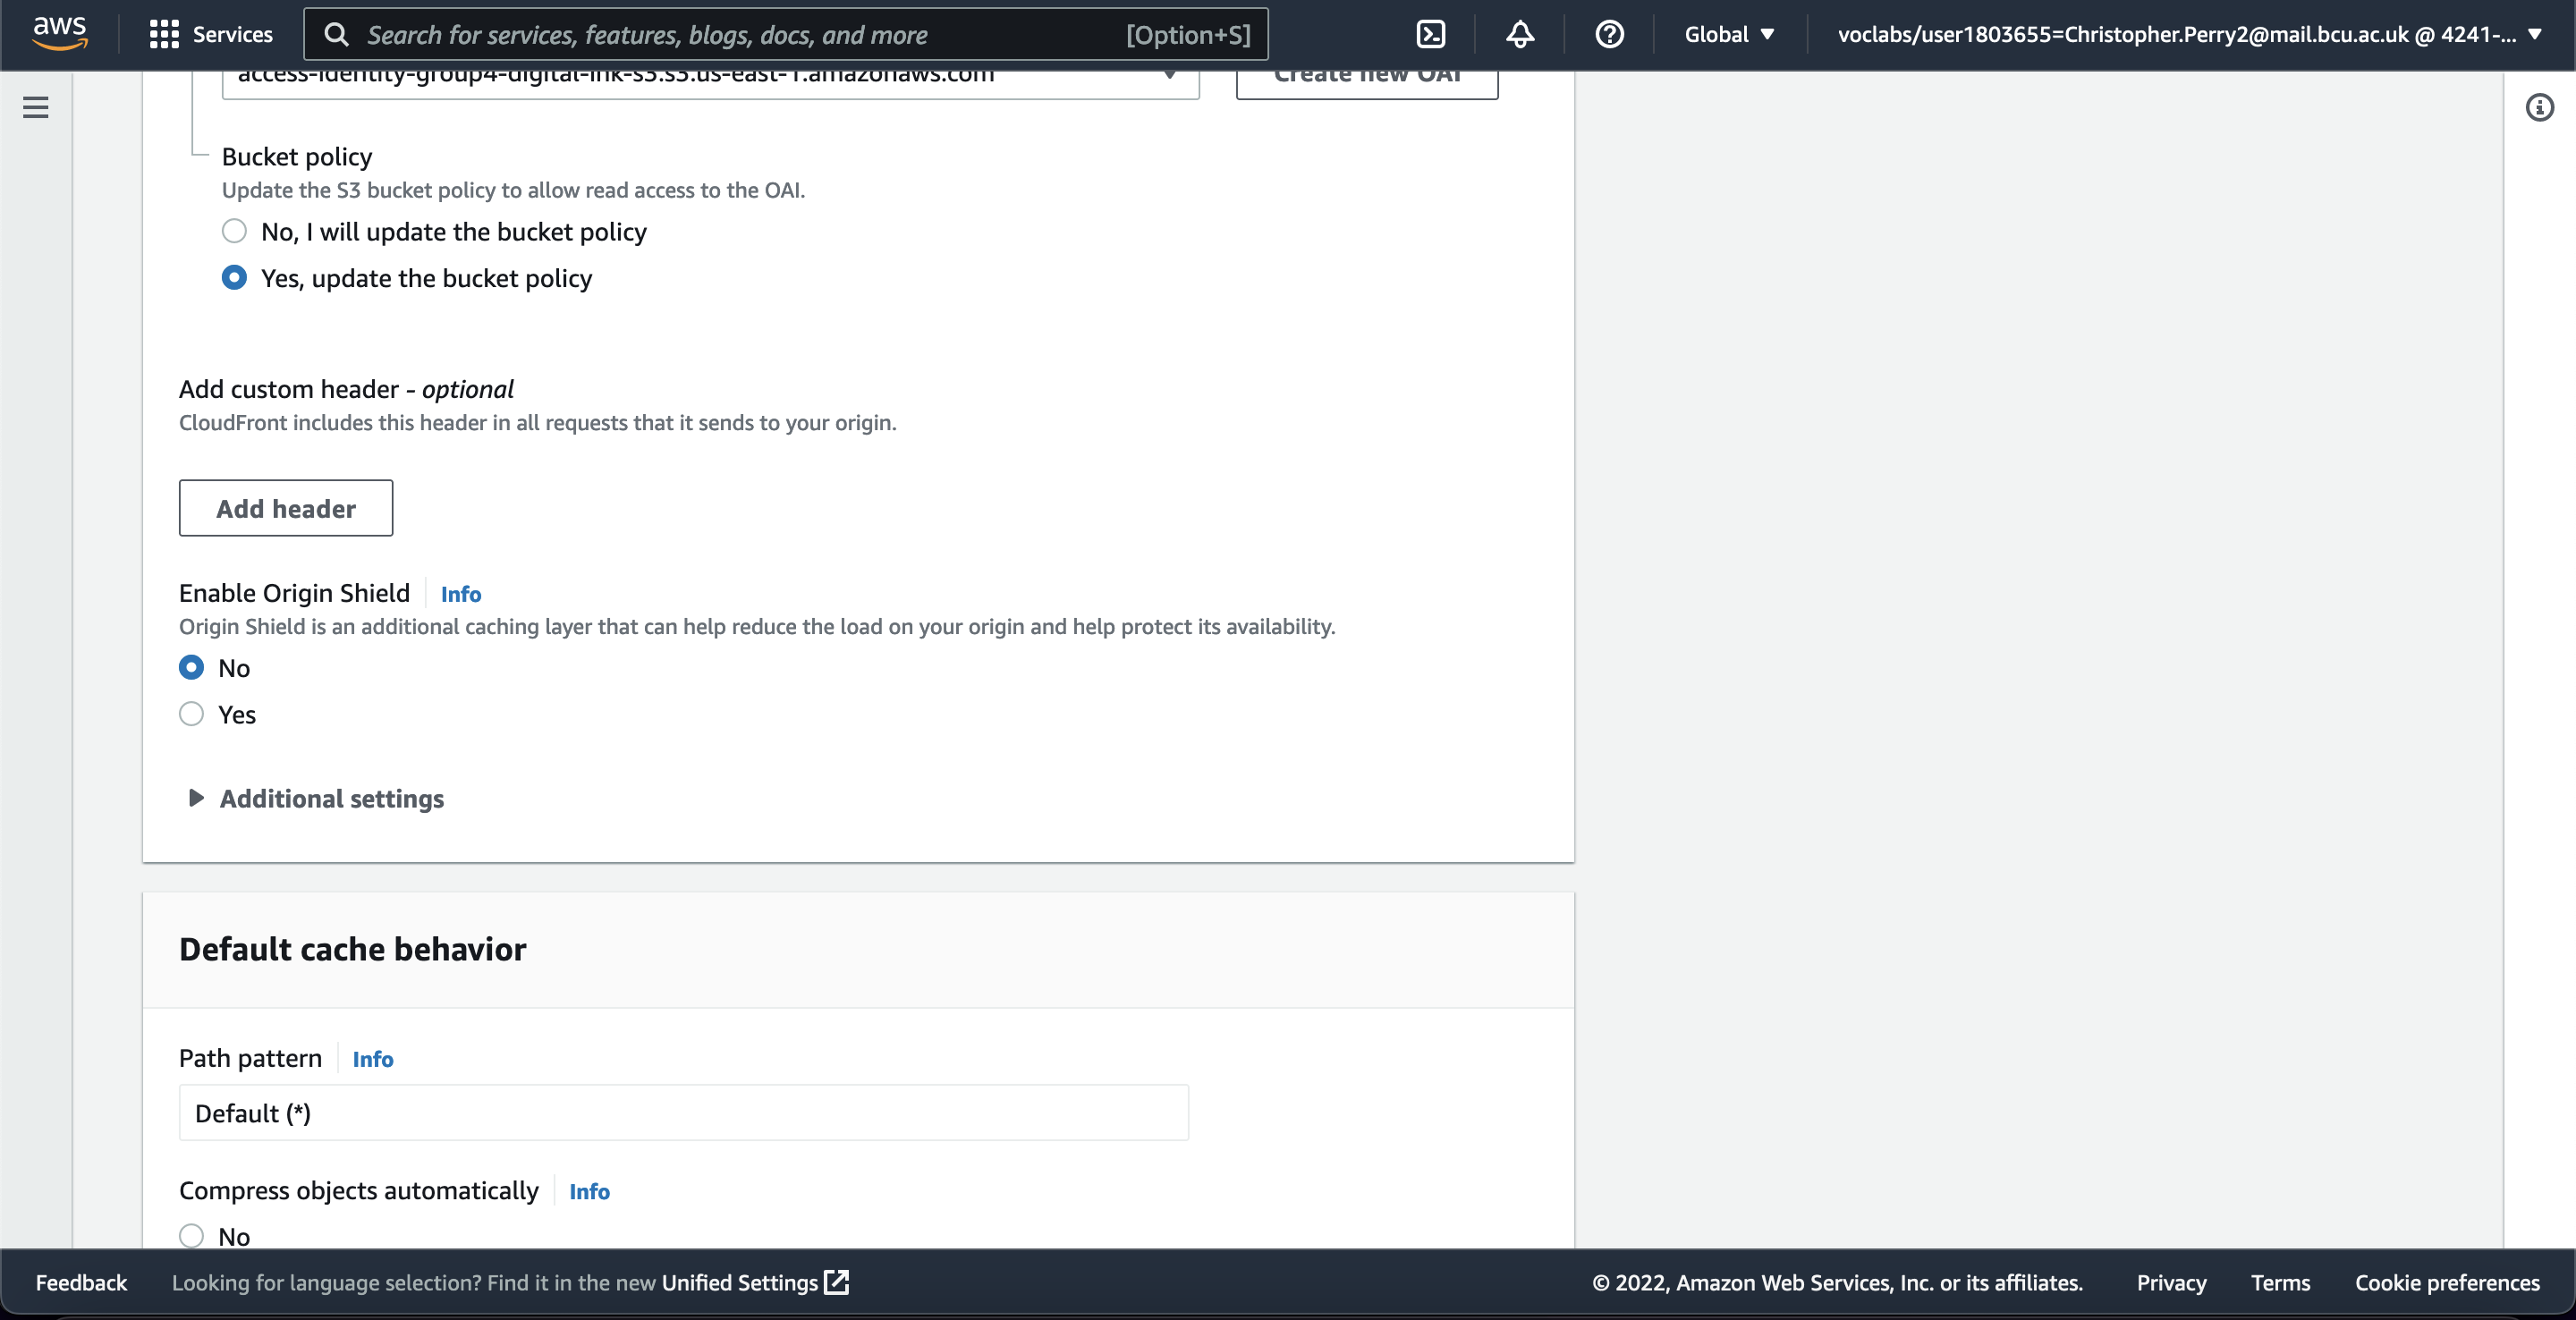
\includegraphics[width=\textwidth]{resources/cloudfront/cloudfront-bucket-policy}
    \caption{Applying CloudFront bucket policy.}
    \label{fig:cloudfront-bucket-policy}
\end{figure}

\begin{figure}[!htbp]
    \centering
    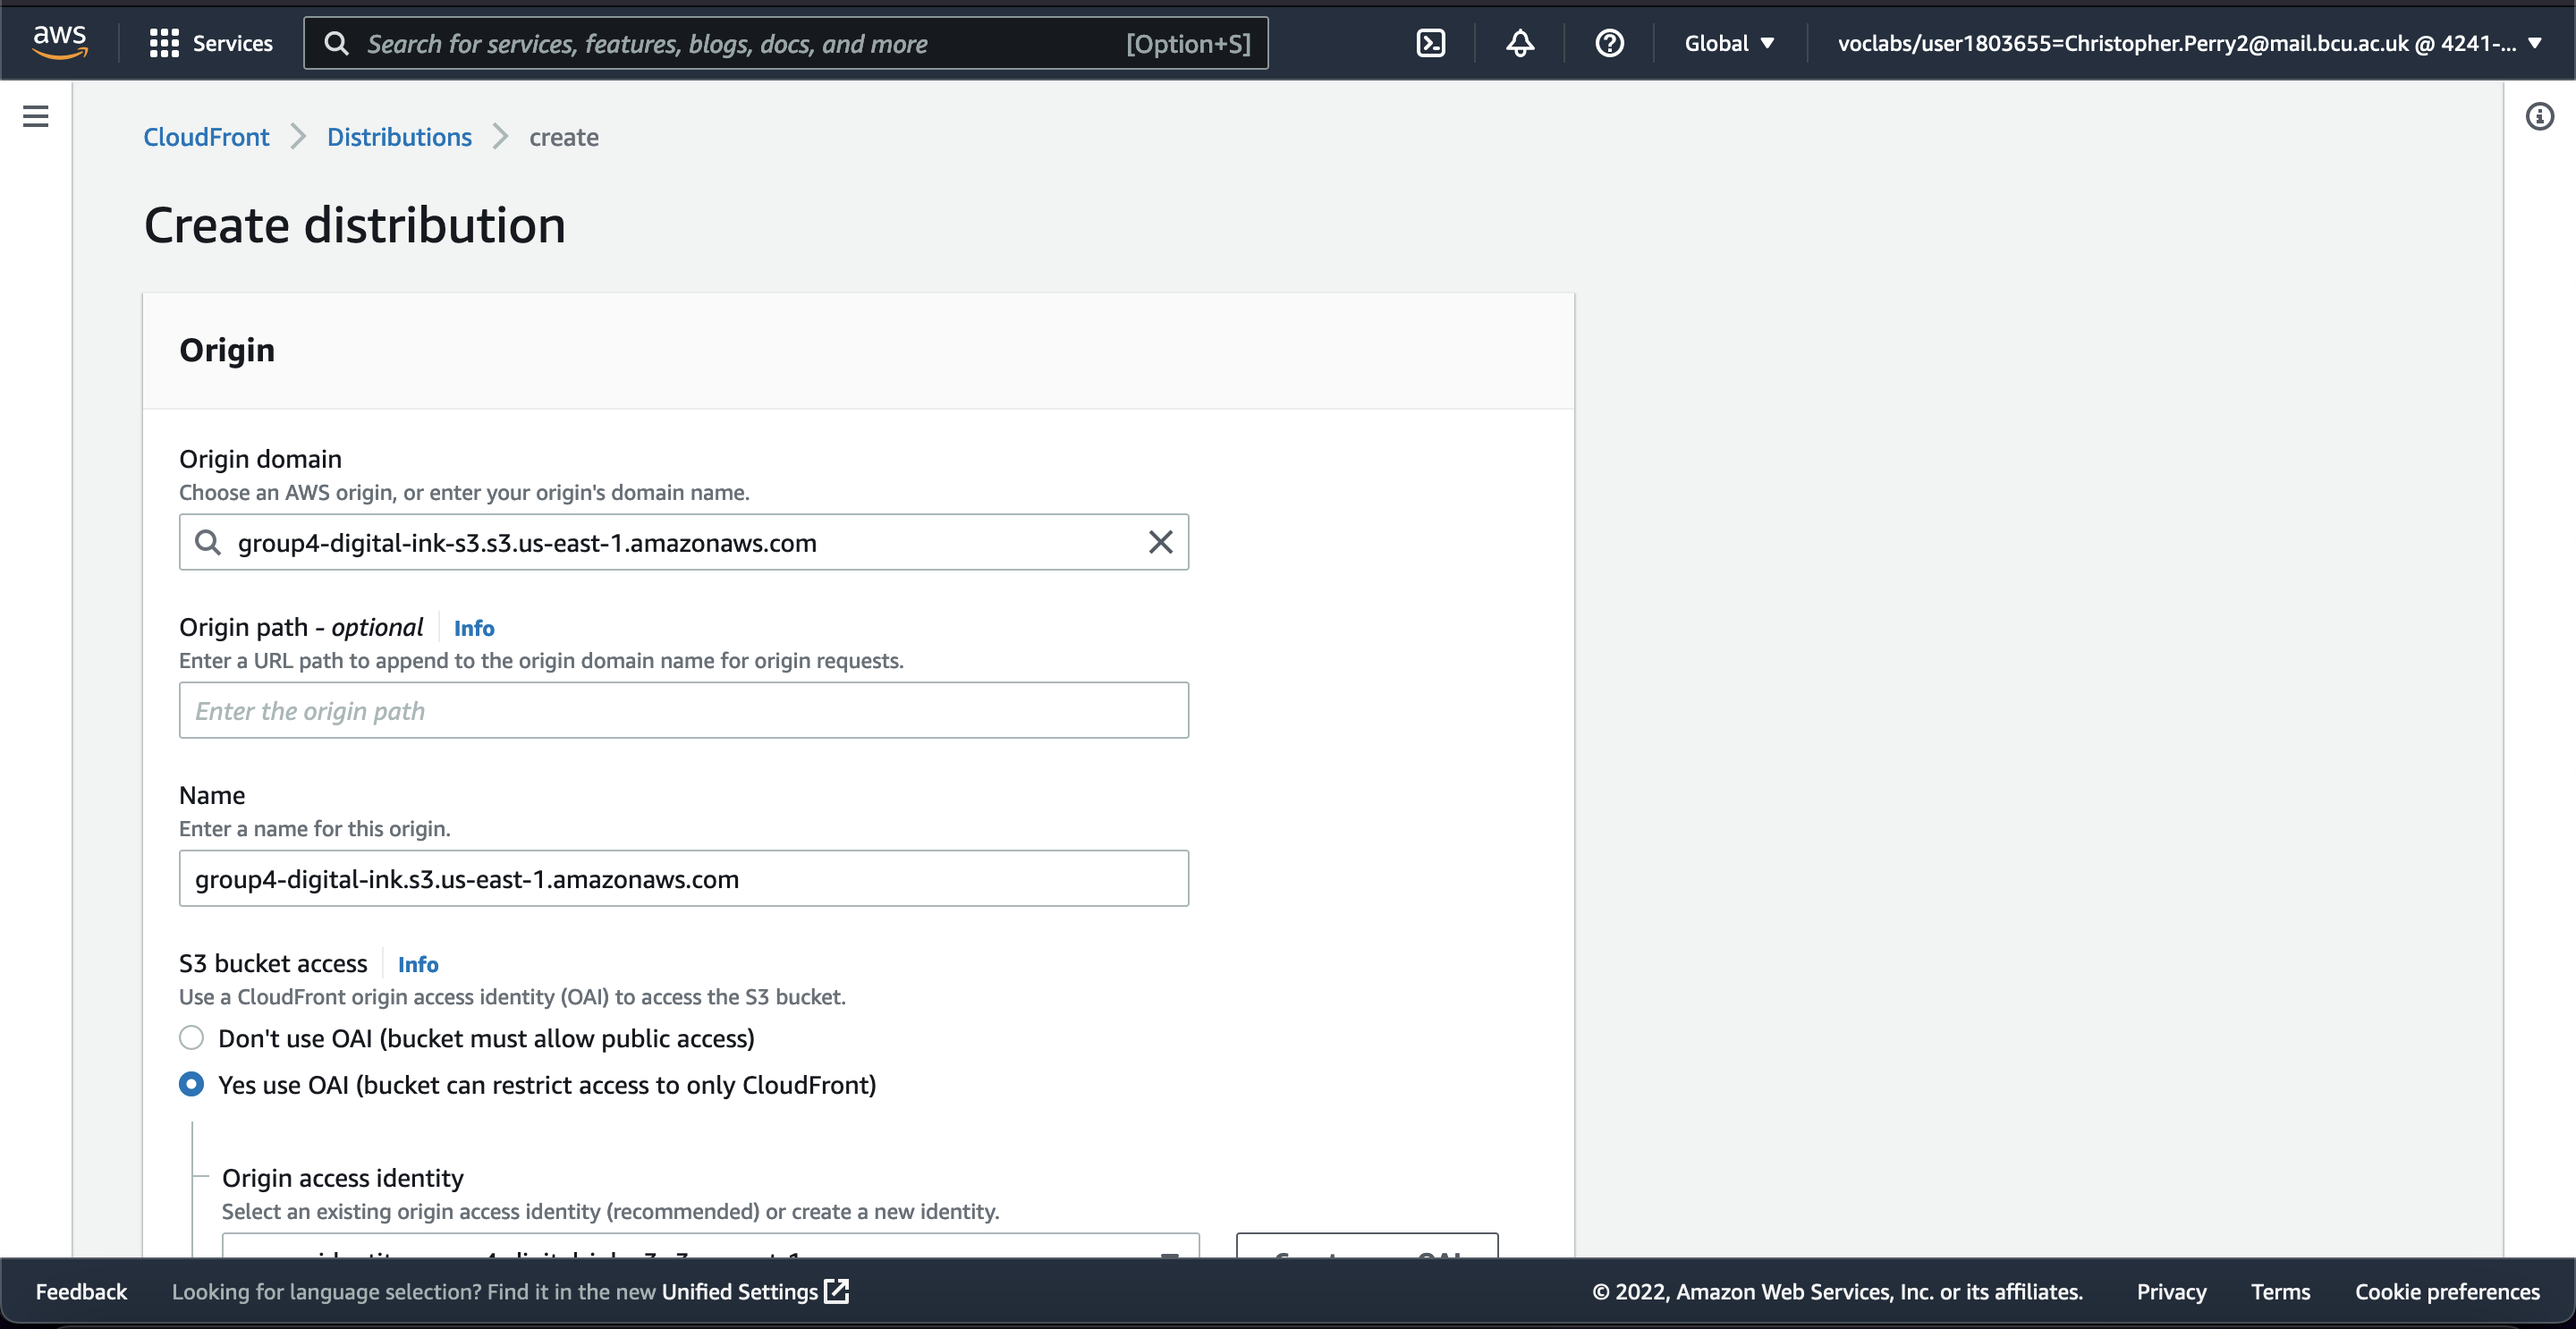
\includegraphics[width=\textwidth]{resources/cloudfront/cloudfront-origin}
    \caption{Applying CloudFront origins to S3 bucket.}
    \label{fig:cloudfront-origins}
\end{figure}

\clearpage

Permissions are then applied to the CloudFront distribution itself.
Objects are set to be compressed automatically to save space, and for viewing images, permissions are set to be in
both HTTP and HTTPS, and to only allow \mintinline{zsh}|GET| and \mintinline{zsh}|HEAD|, so images can only be viewed.

\begin{figure}[!htbp]
    \centering
    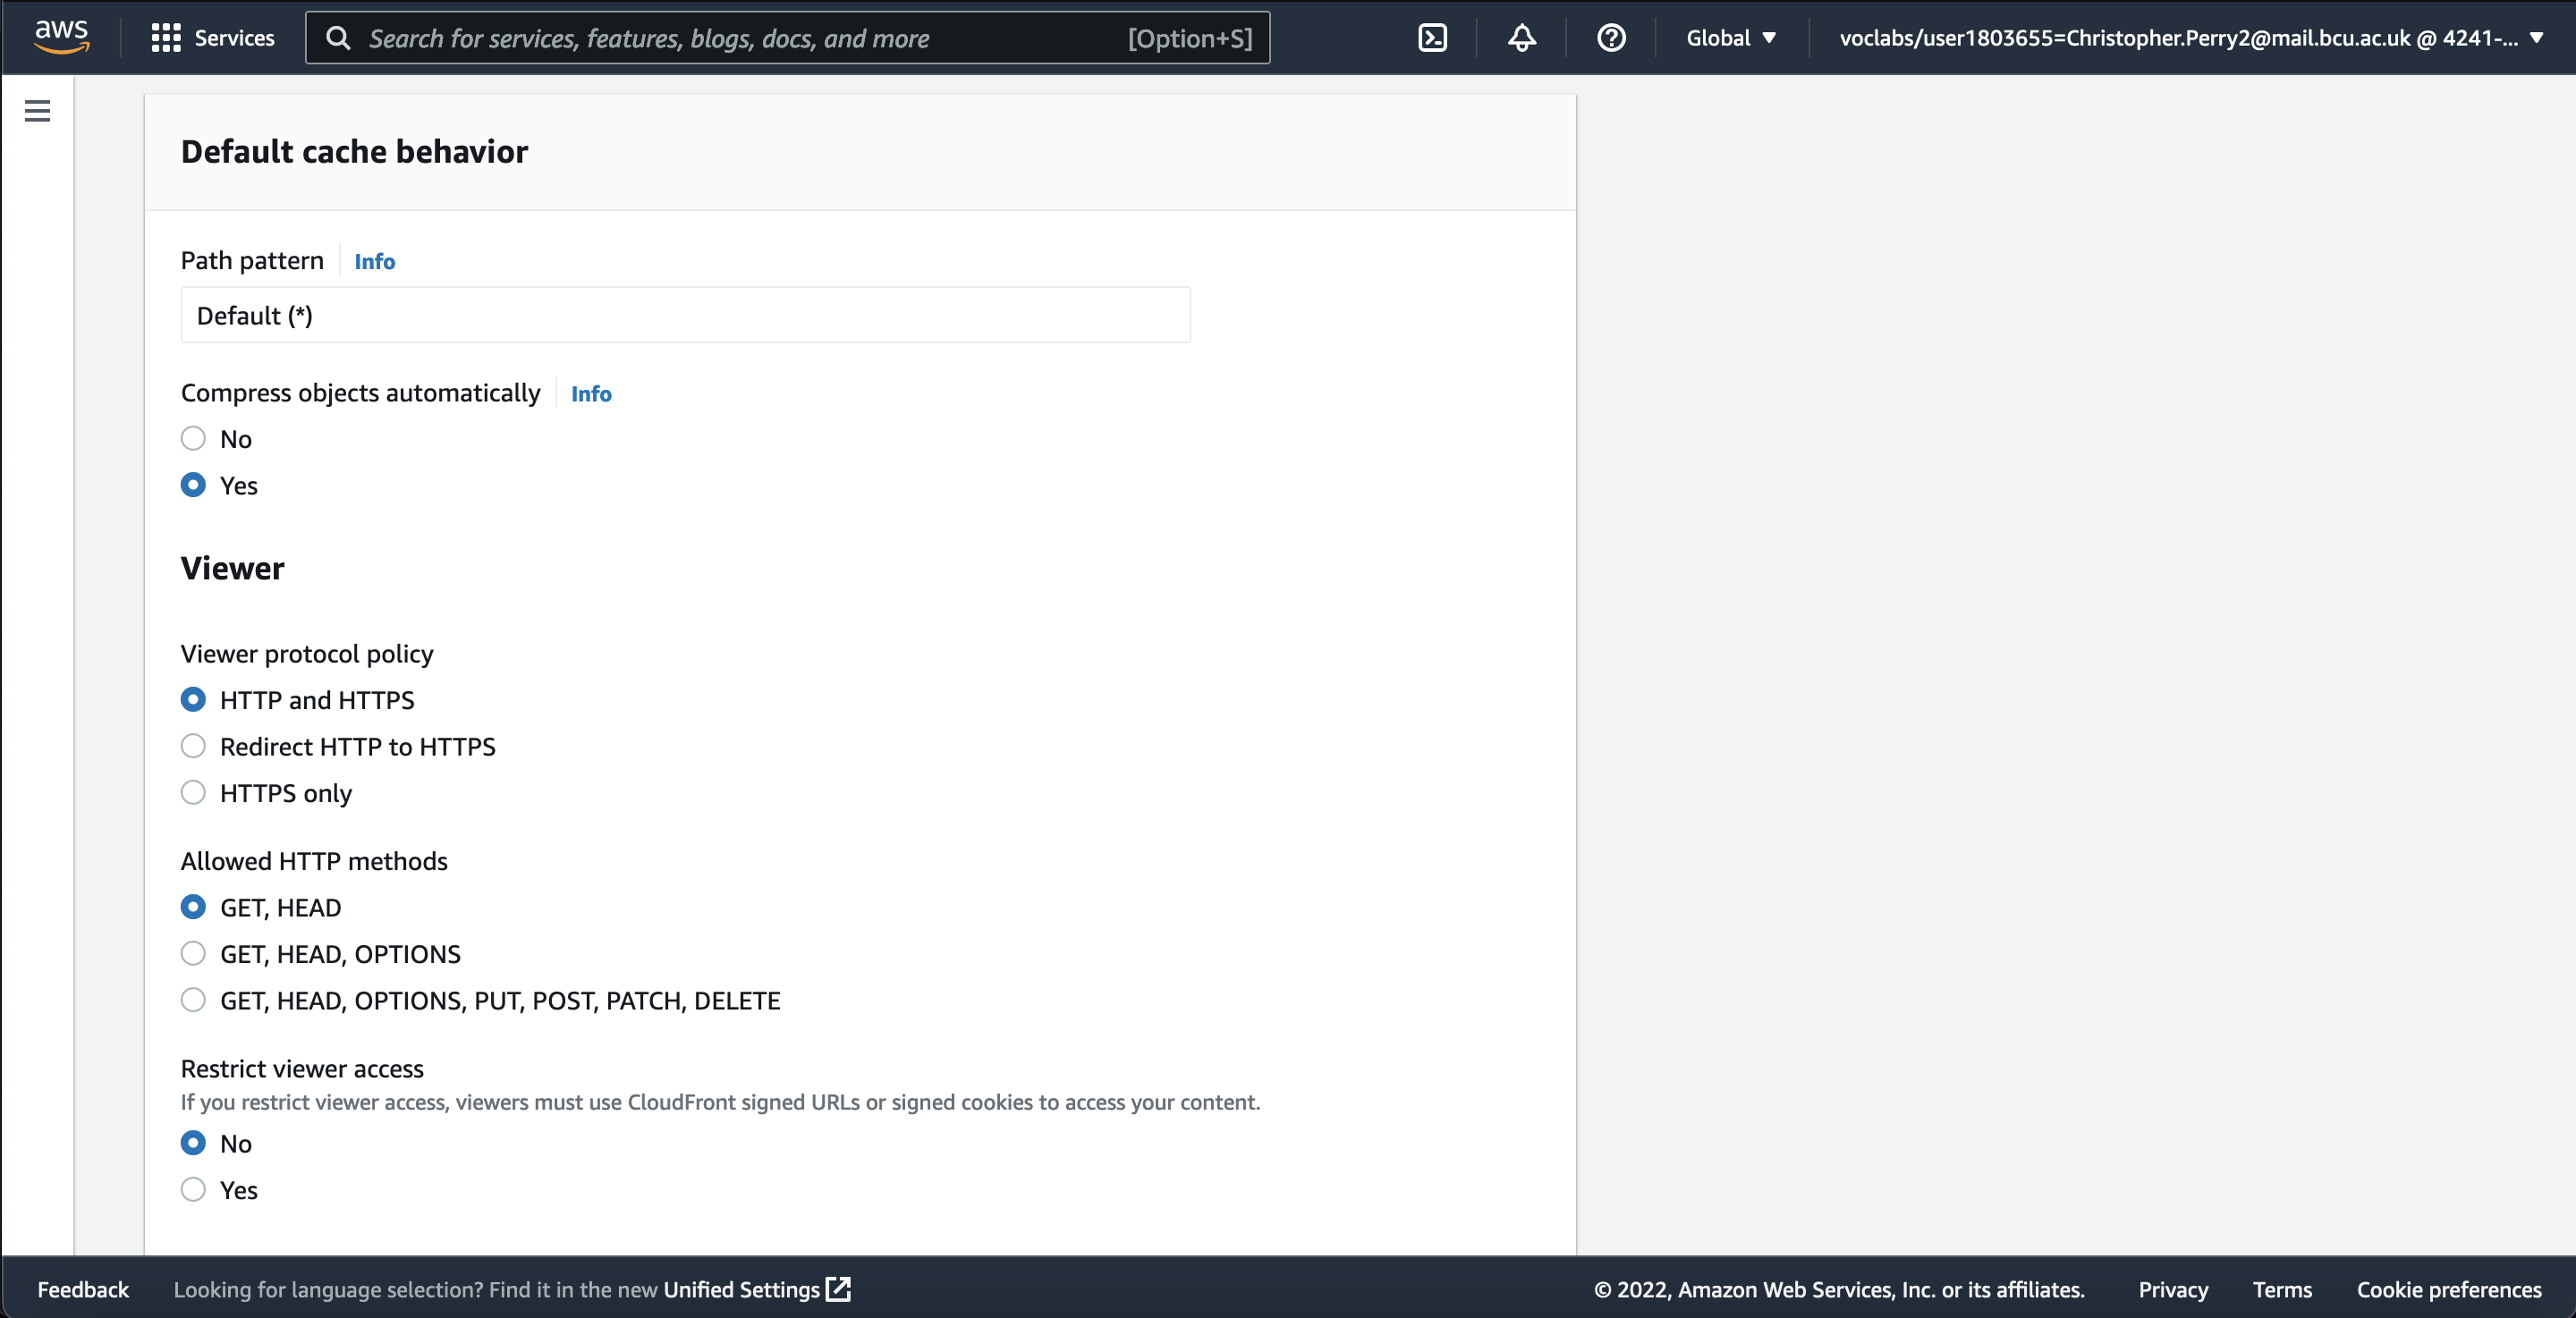
\includegraphics[width=\textwidth]{resources/cloudfront/cloudfront-cache-behaviour}
    \caption{Applying CloudFront Distribution Permissions.}
    \label{fig:cloudfront-cache-behaviour}
\end{figure}

A cache policy and origin request policy is subsequently applied to the aforementioned permissions.
The "CachingOptimized" policy is applied for compression.
Origin Request policy is set to "CORS-S3Origin" in order for CORS to be automatically set up for the S3 bucket,
Any GET requests are then compatible in the response headers through "SimpleCORS".

\begin{figure}[!htbp]
    \centering
    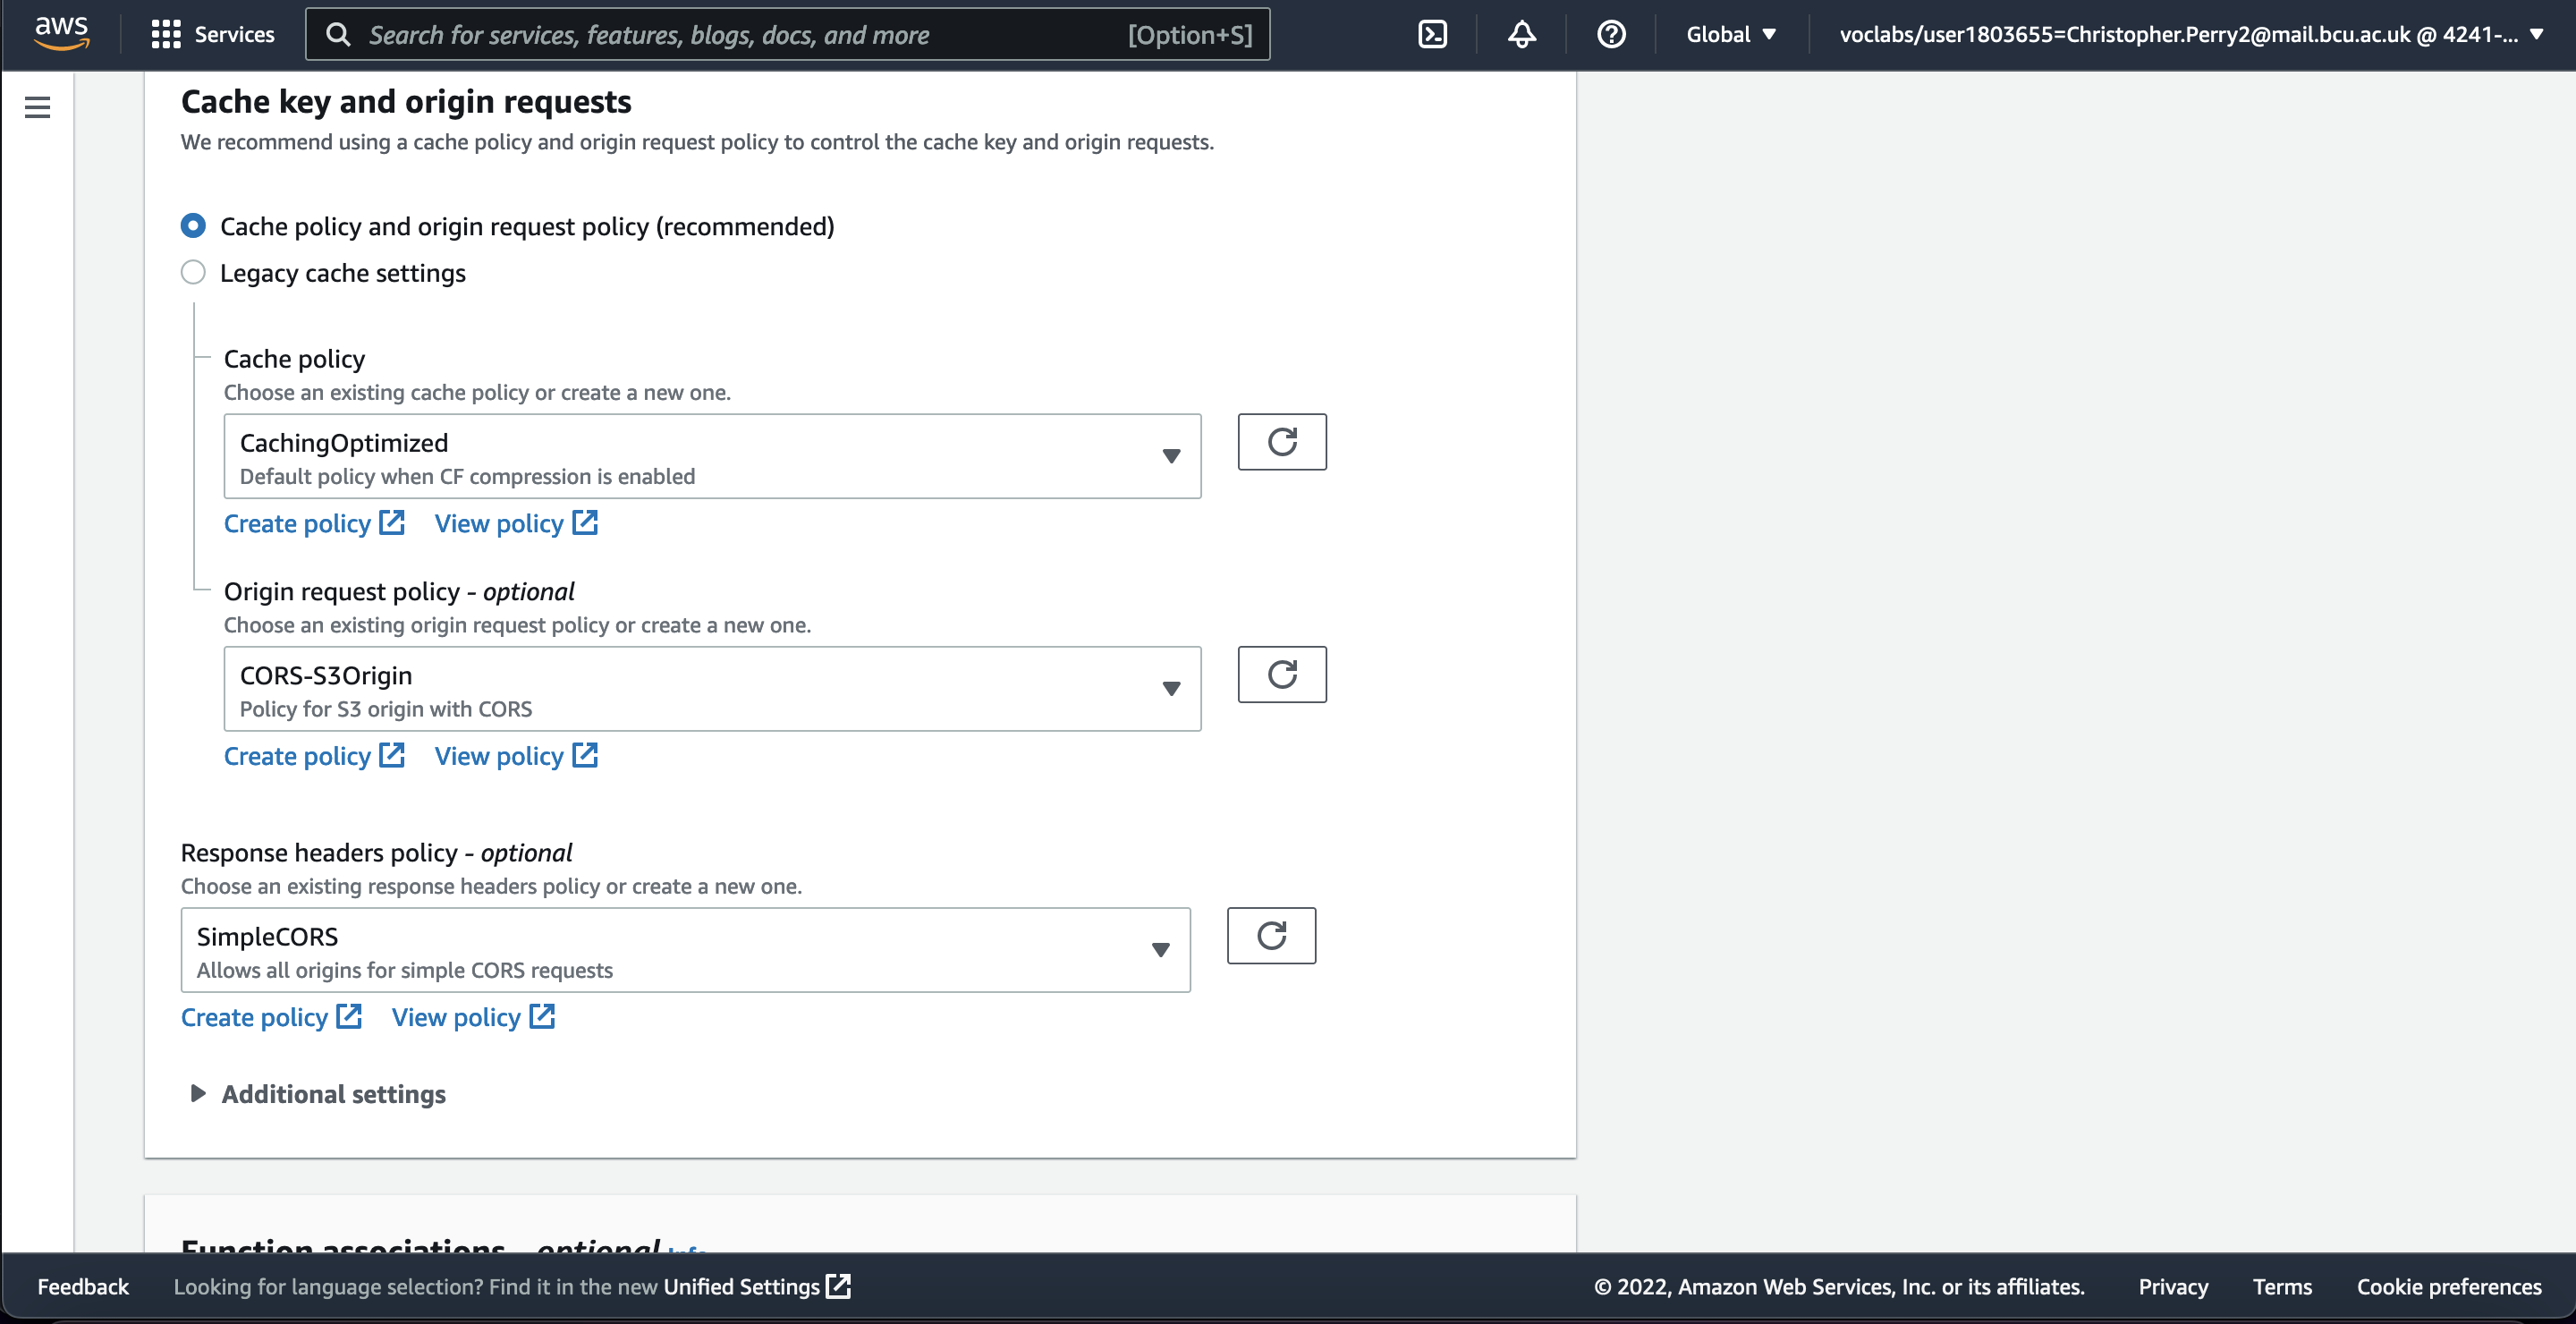
\includegraphics[width=\textwidth]{resources/cloudfront/cloudfront-cache-key}
    \caption{Applying CloudFront Cache Keys and Origin Requests.}
    \label{fig:cloudfront-cache-key}
\end{figure}

No function associations are set due to the lack of CloudFront functions and Lambdas.

\begin{figure}[!htbp]
    \centering
    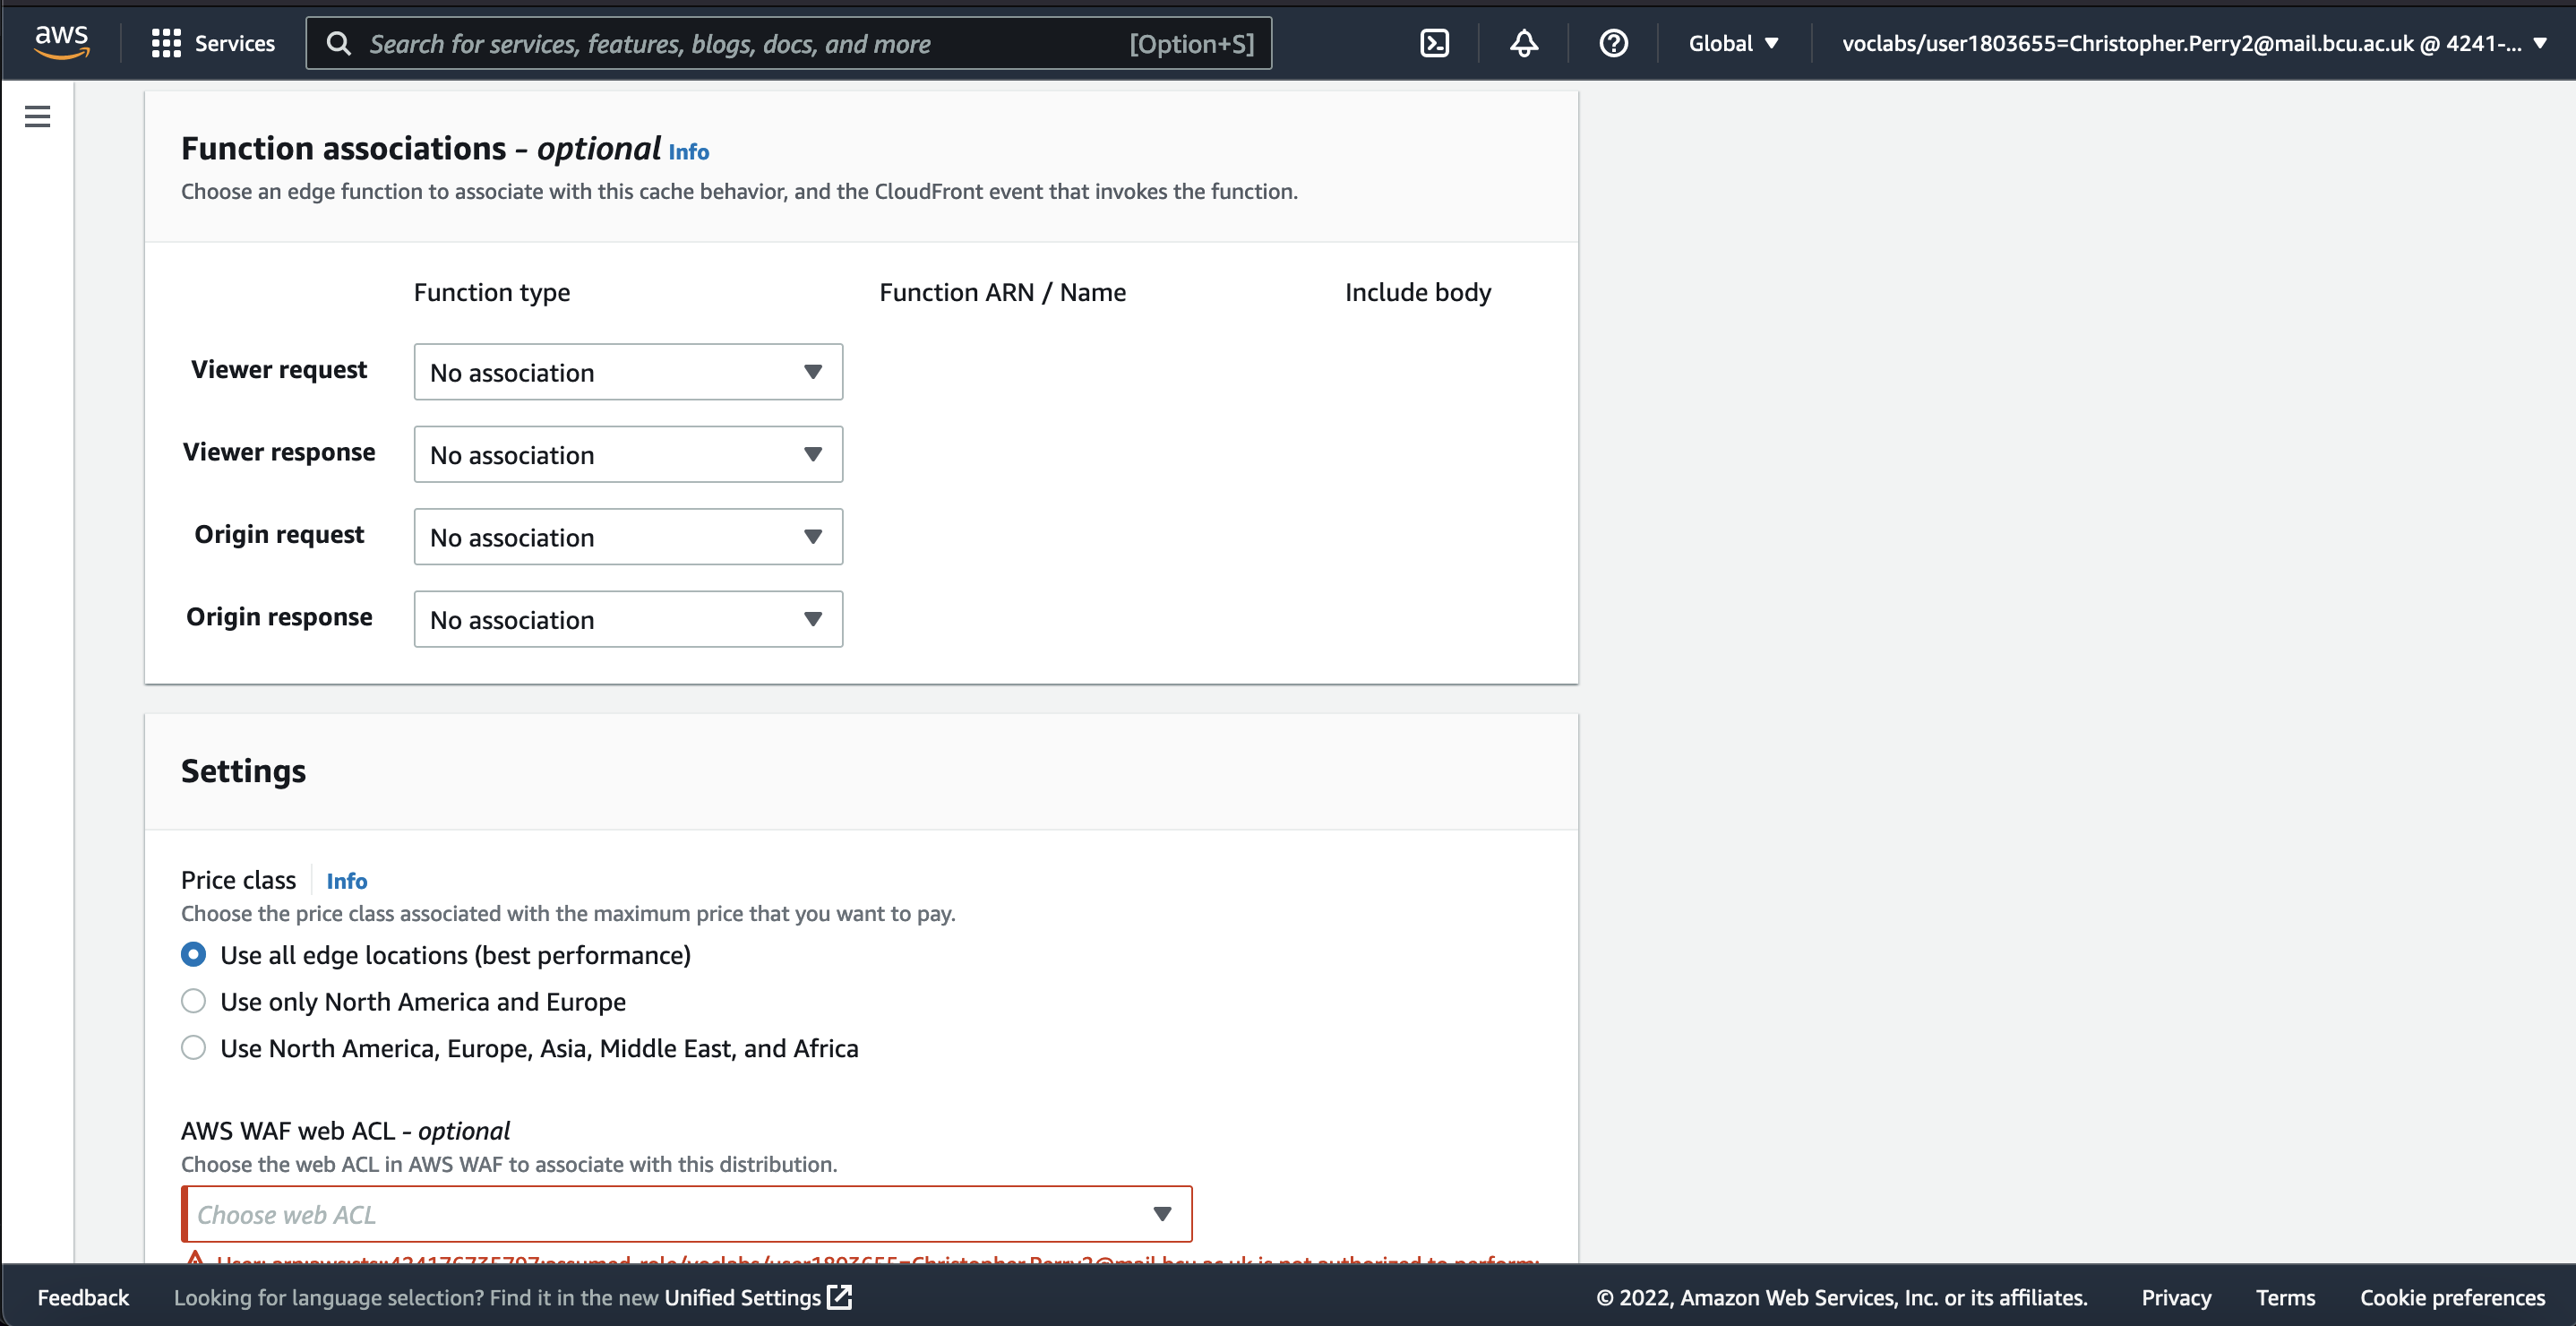
\includegraphics[width=\textwidth]{resources/cloudfront/cloudfront-function-association}
    \caption{Function Association.}
    \label{fig:cloudfront-function-association}
\end{figure}

The settings for the CloudFront Distribution can now be set.
In order to ensure high availability, the option "Use all edge locations" is selected, so that images can be distributed
to the user from the closest edge location in relation to their IP address.
No ACL can be added to the WAF due to permissions issues, and a SSL Certificate cannot be set as the web app is not being
served from the internet.
For logging purposes "Standard Logging" is set to "On", and logs are saved to the same S3 bucket.
Cookie logging is enabled, and IPv6 is set to "On", to allow for more IP addresses to access the CloudFront Distributed
content.
These settings can be found in Figures~\ref{fig:cloudfront-setting-1} and~\ref{fig:cloudfront-setting-2}.

\clearpage

\begin{figure}[!htbp]
    \centering
    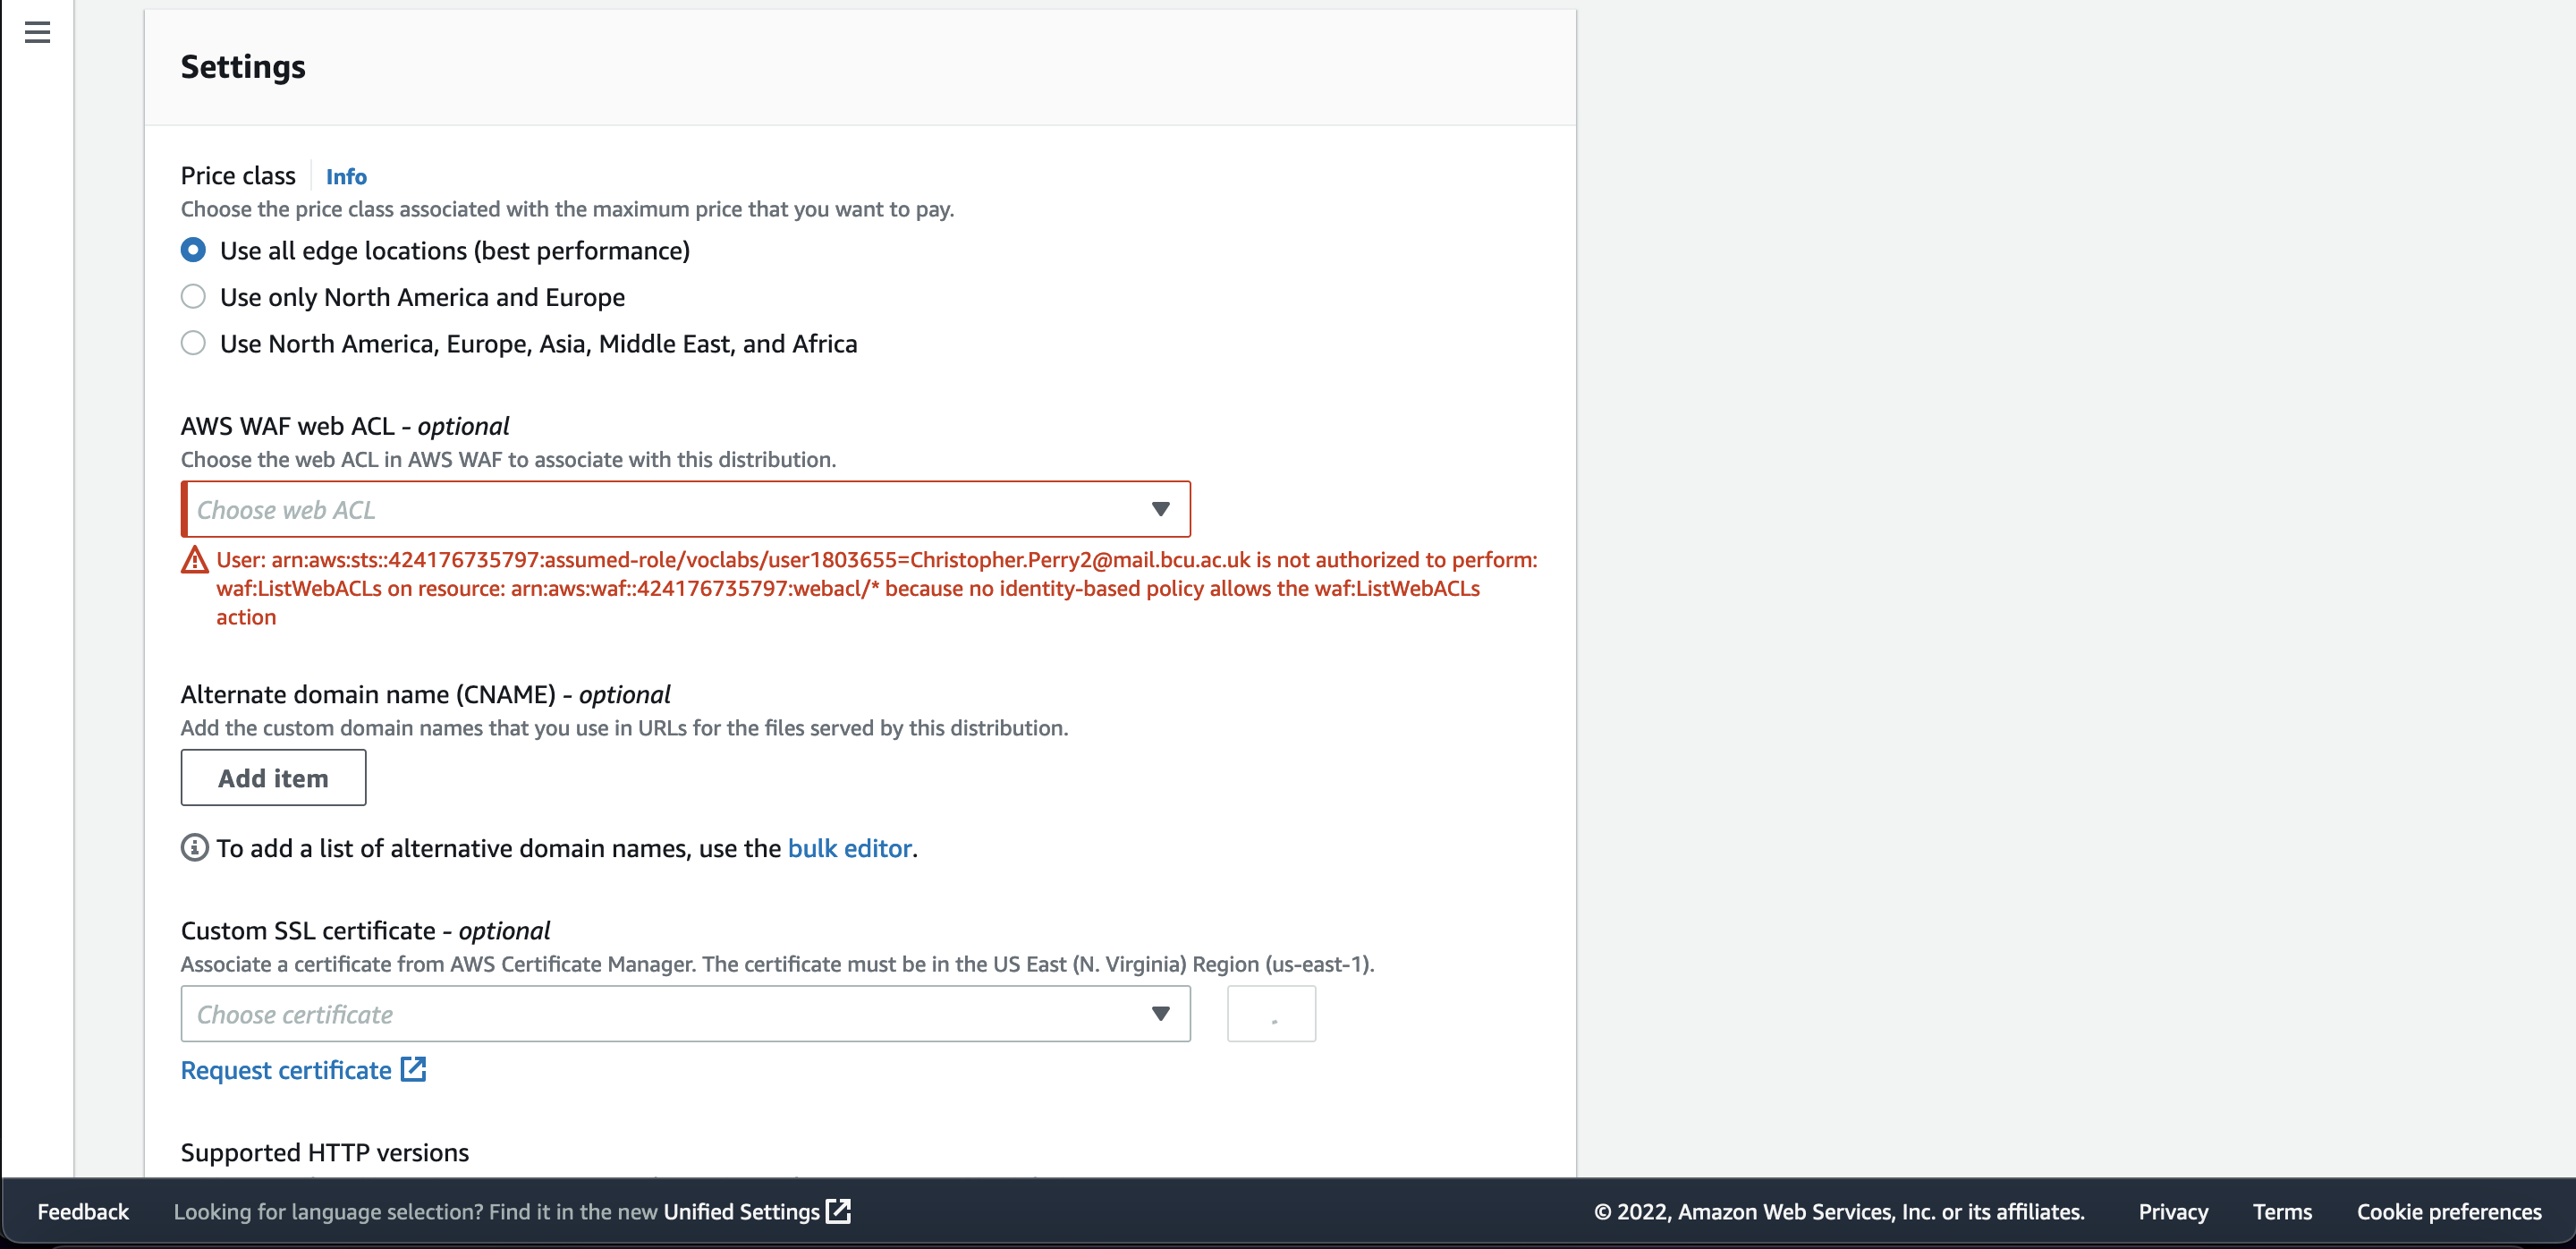
\includegraphics[width=\textwidth]{resources/cloudfront/cloudfront-settings-1}
    \caption{Applying CloudFront Settings.}
    \label{fig:cloudfront-settings-1}
\end{figure}

\begin{figure}[!htbp]
    \centering
    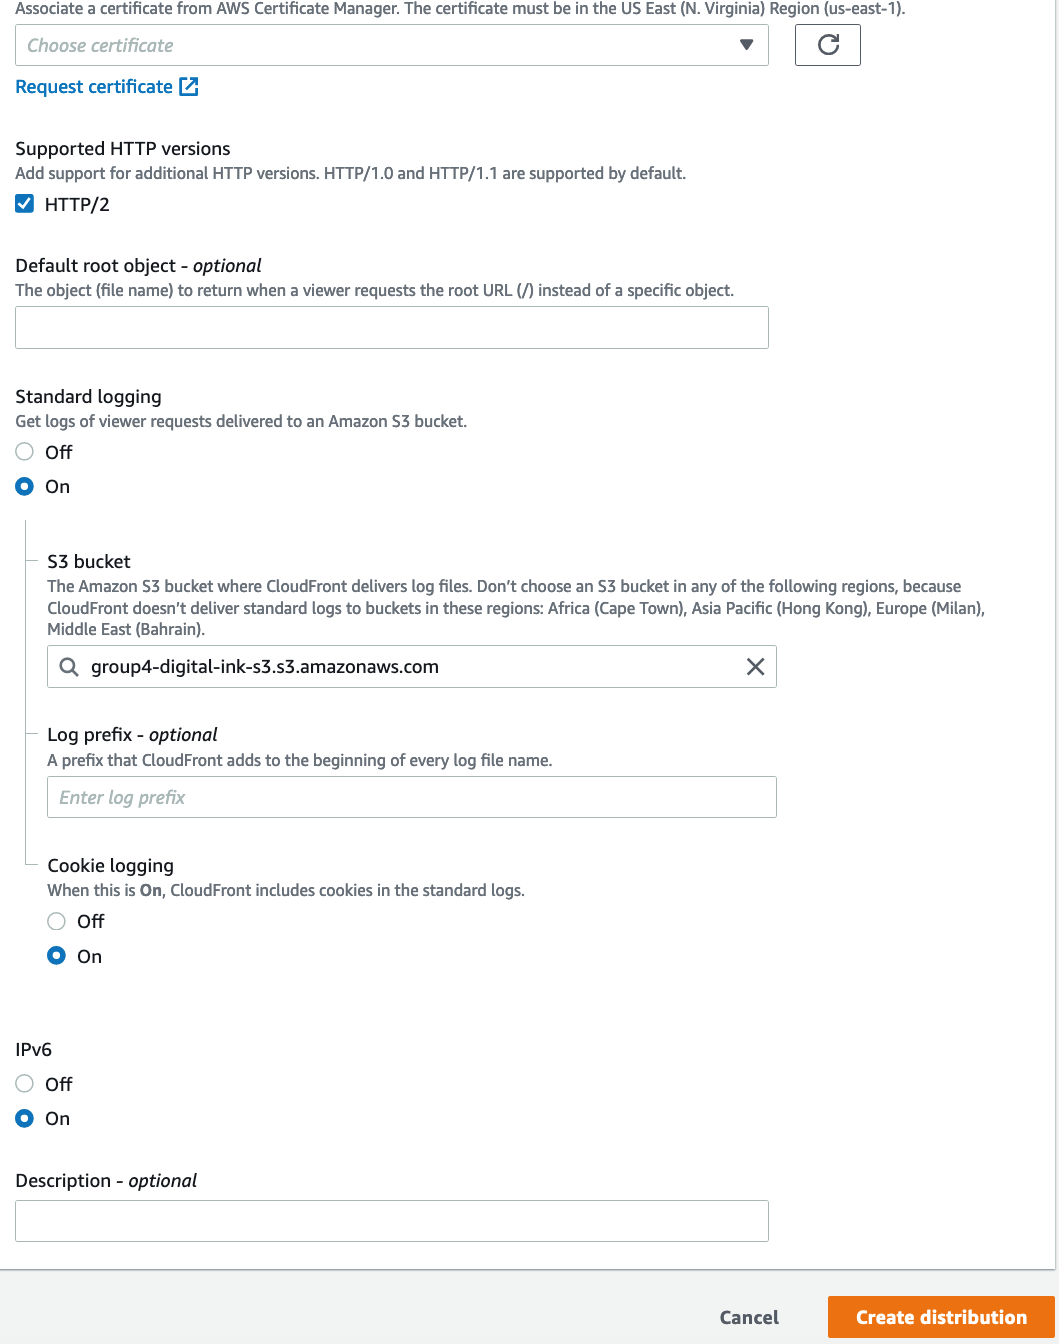
\includegraphics[width=\textwidth]{resources/cloudfront/cloudfront-settings-2}
    \caption{Applying CloudFront Settings.}
    \label{fig:cloudfront-setting-2}
\end{figure}

\clearpage

A CloudFront Distribution has now been created, and can be found in Figure~\ref{fig:cloudfront-created}.

\begin{figure}[!htbp]
    \centering
    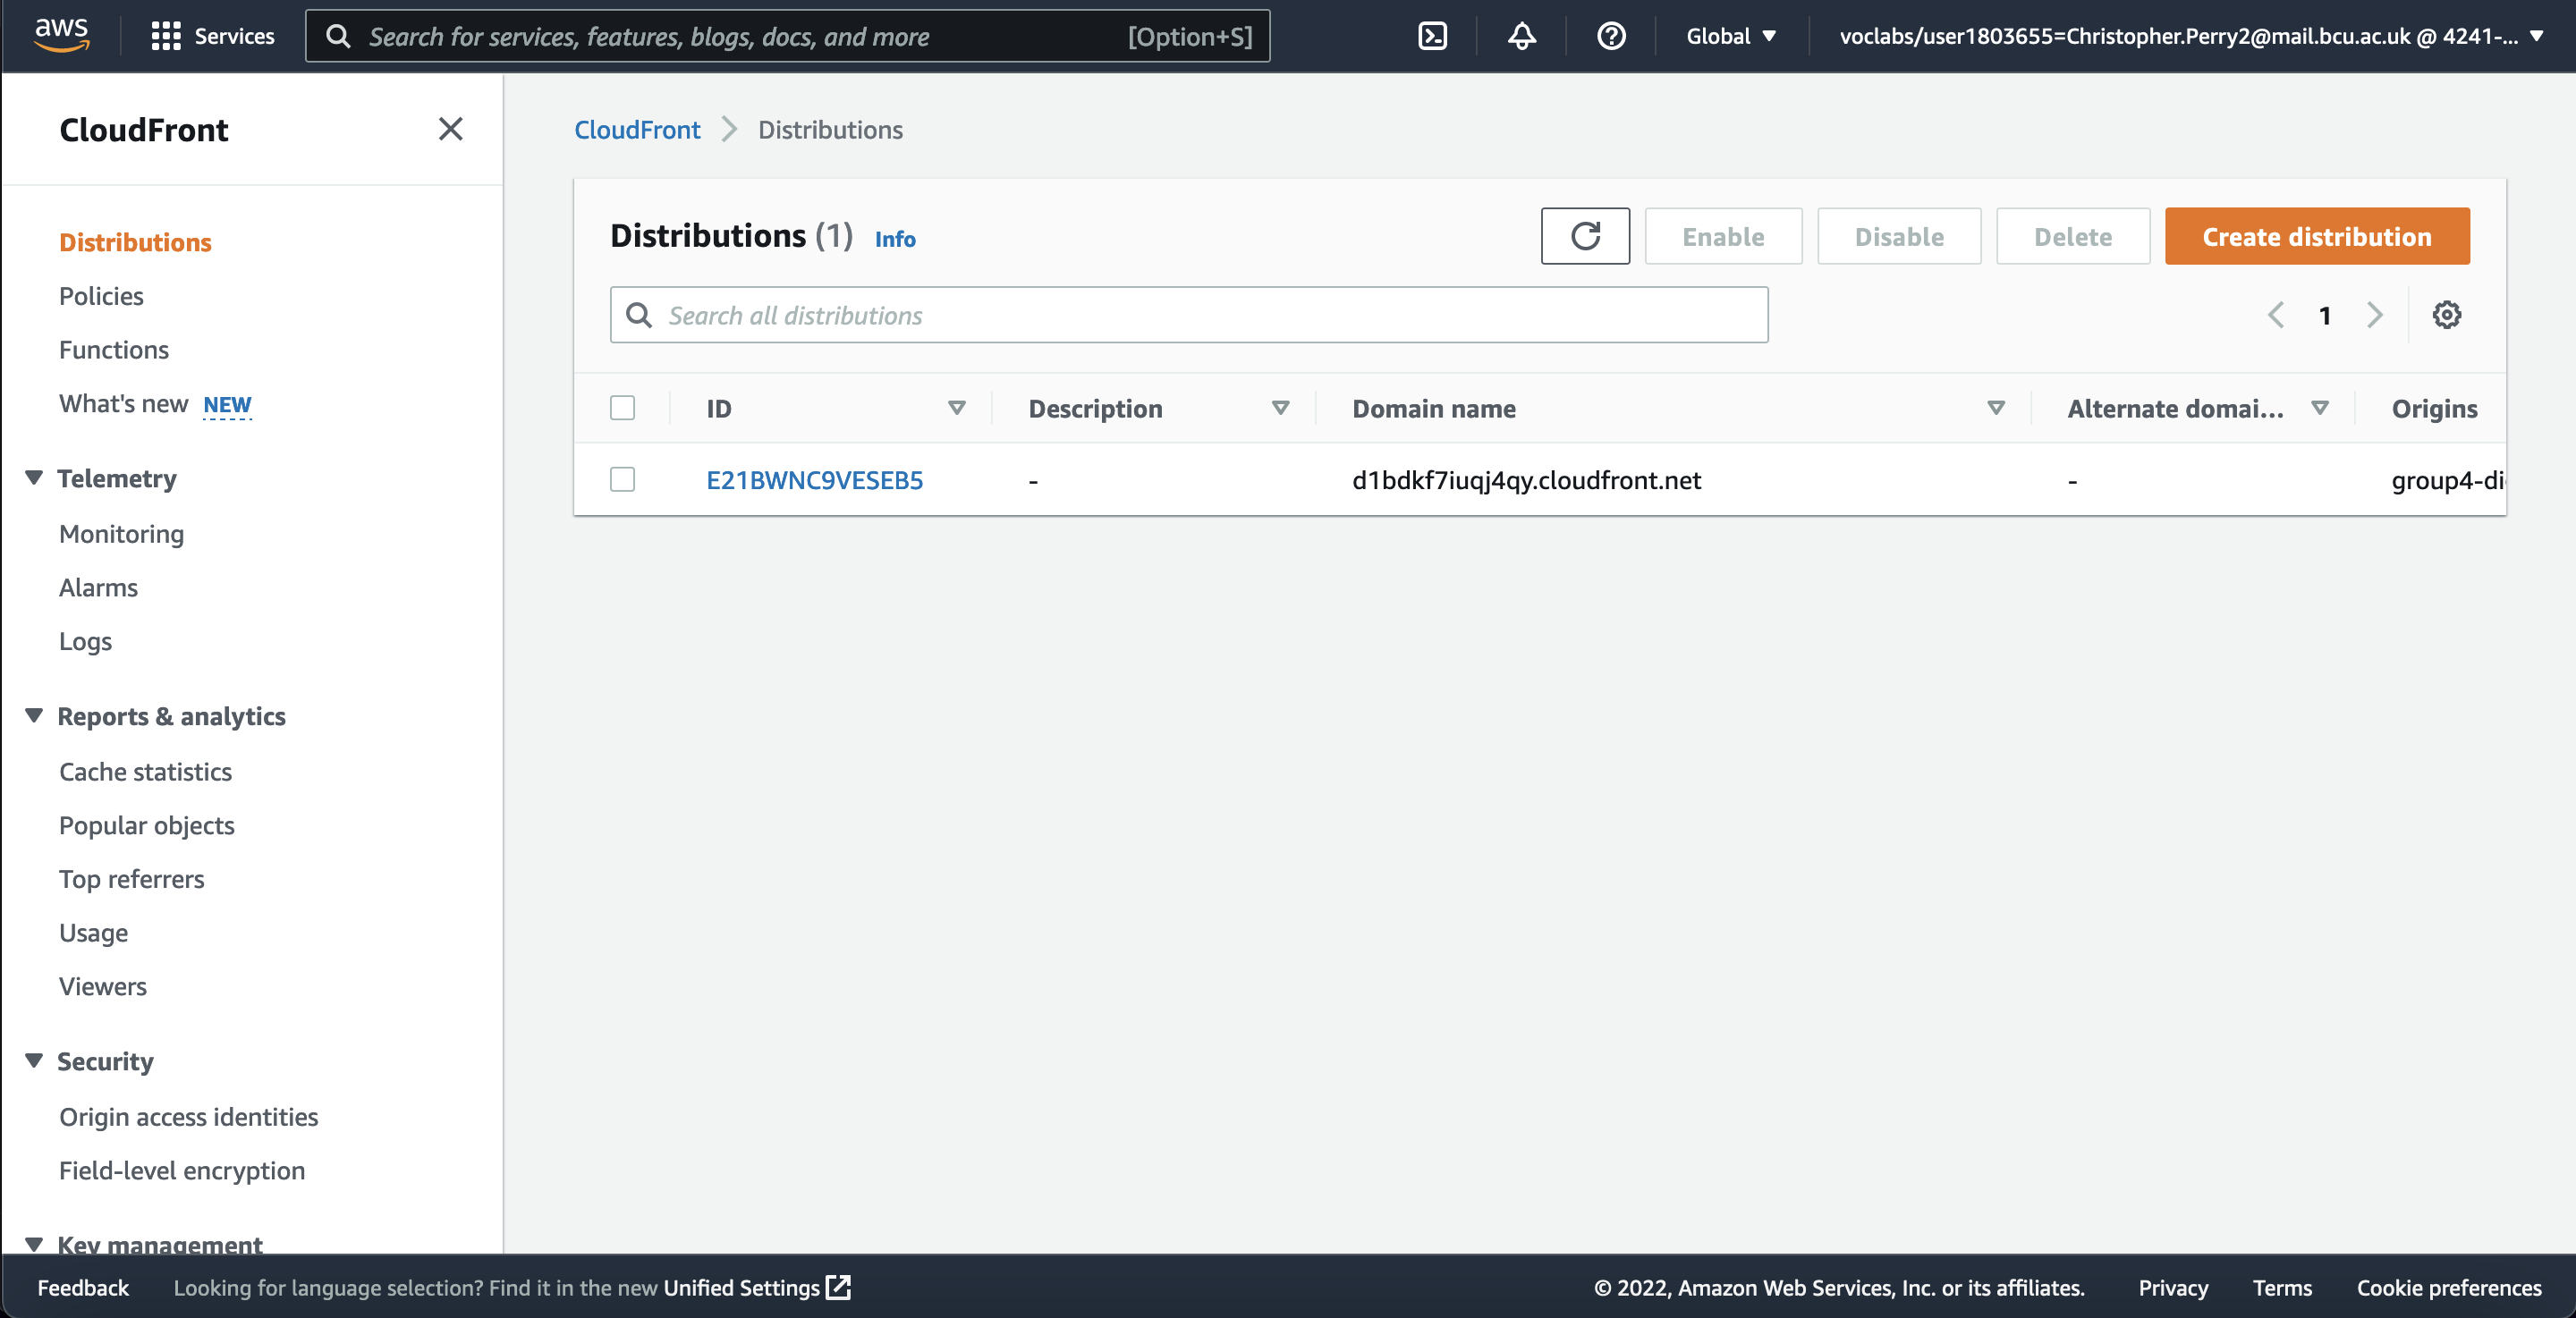
\includegraphics[width=\textwidth]{resources/cloudfront/cloudfront-created}
    \caption{Created CloudFront Distribution.}
    \label{fig:cloudfront-created}
\end{figure}

Finally, the images contained within the webserver were changed from their local location to their relevant CloudFront
locations.
This change can be seen in Figures~\ref{fig:cloudfront-before} and~\ref{fig:cloudfront-after}.

\begin{figure}[!htbp]
    \centering
    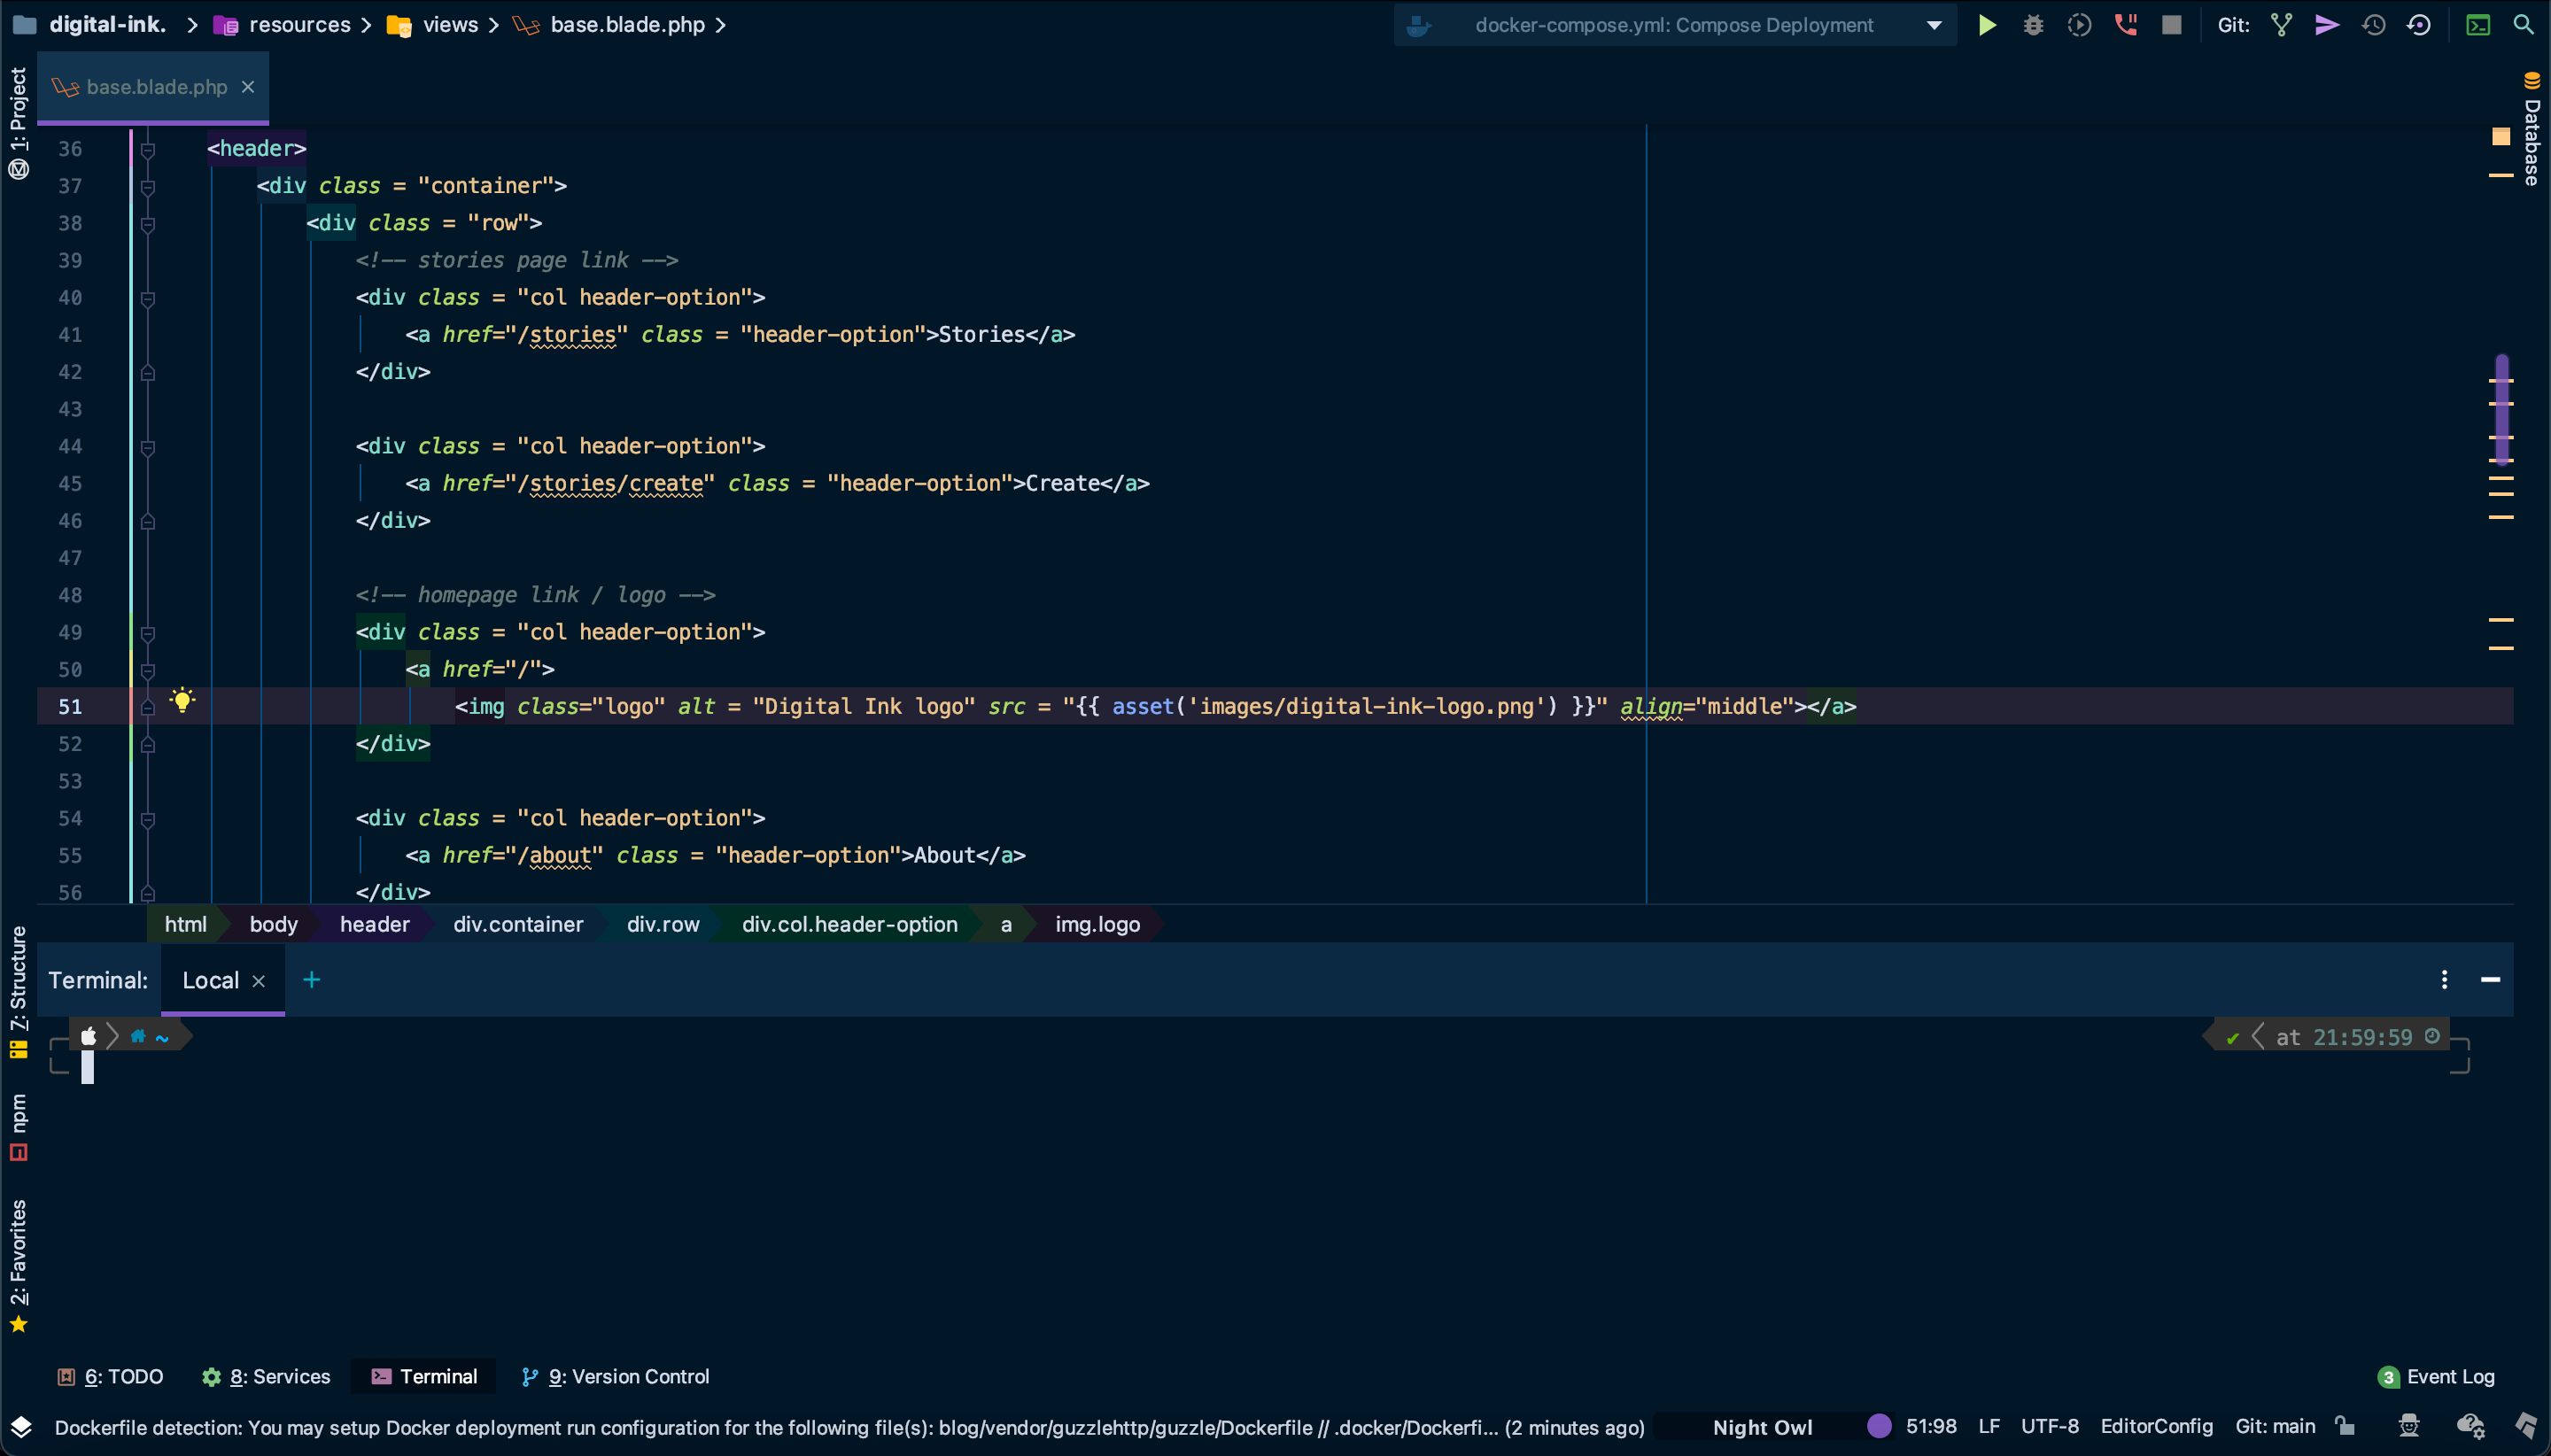
\includegraphics[width=\textwidth]{resources/cloudfront/cloudfront-before}
    \caption{Image location before CloudFront.}
    \label{fig:cloudfront-before}
\end{figure}

\begin{figure}[!htbp]
    \centering
    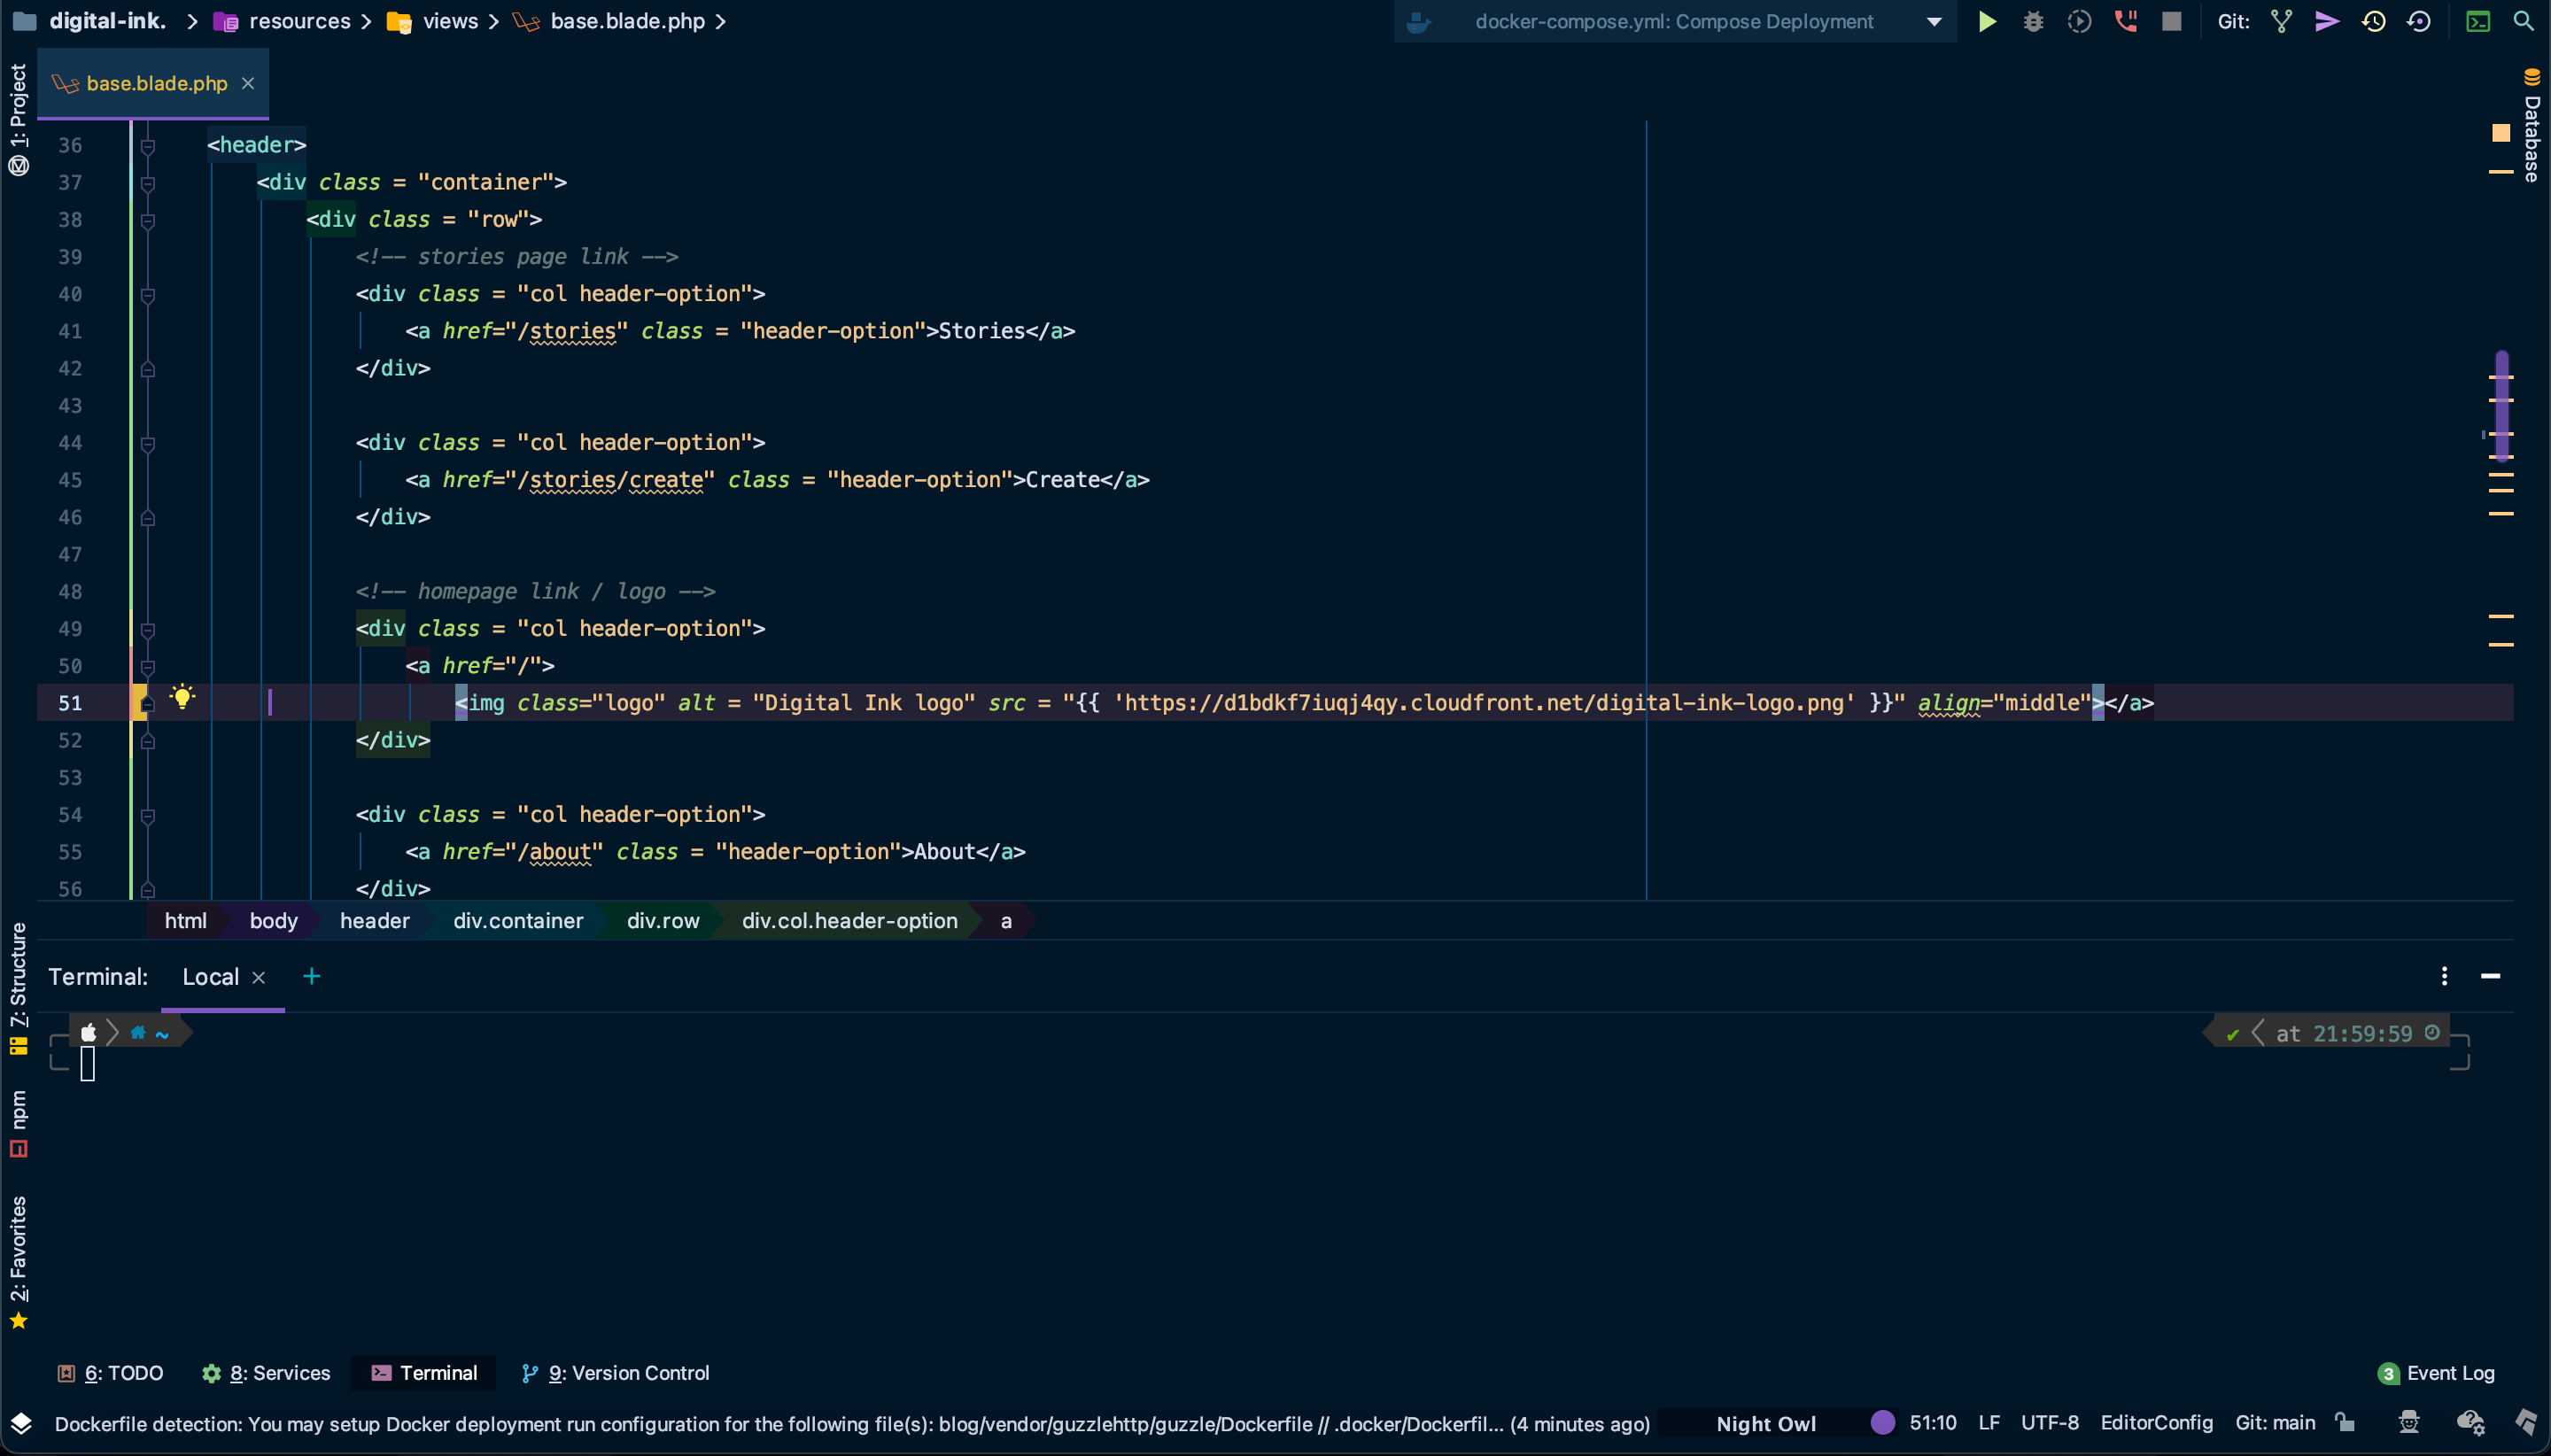
\includegraphics[width=\textwidth]{resources/cloudfront/cloudfront-after}
    \caption{Image location after CloudFront.}
    \label{fig:cloudfront-after}
\end{figure}

\clearpage

\begin{figure}[!htbp]
    \centering
    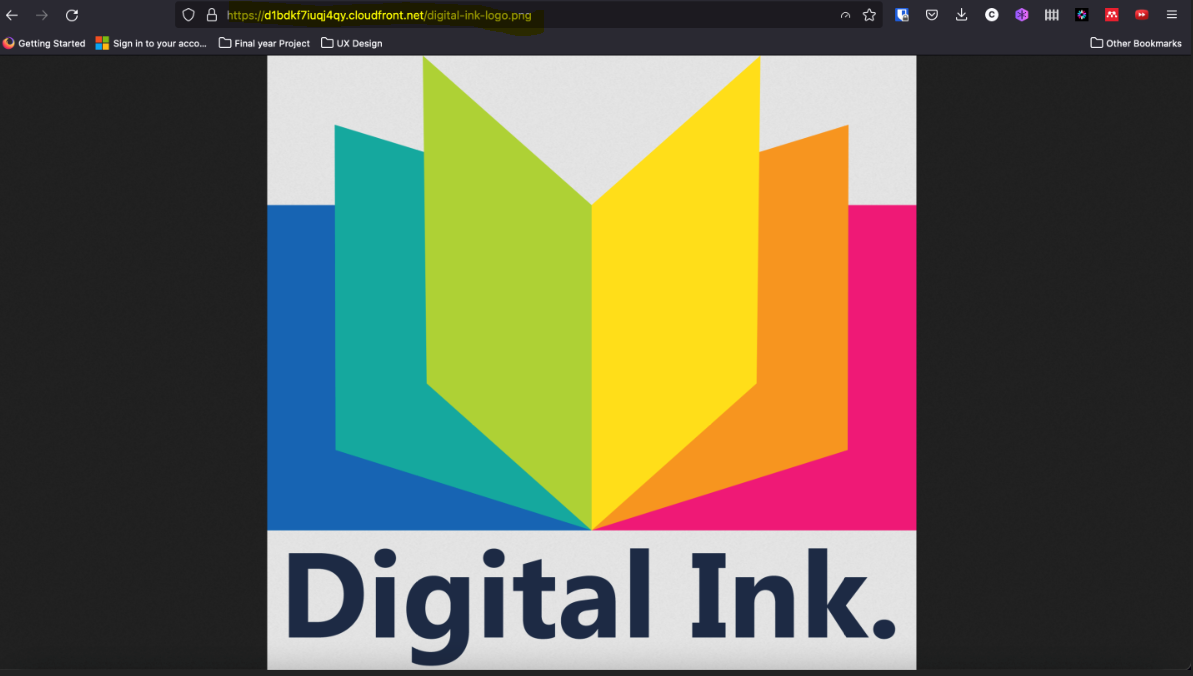
\includegraphics[width=\textwidth]{resources/cloudfront/cloudfront-website}
    \caption{Image location after CloudFront.}
    \label{fig:cloudfront-website}
\end{figure}

As seen in Figure~\ref{fig:cloudfront-website}, the Digital Ink logo is now hosted on CloudFront.






    \chapter{CloudWatch}\label{ch:cloudwatch}

Amazon CloudWatch is a monitoring and observation tool which can provide developers with insights to monitor
applications, react to performance changes, and optimise resource consumption.
CloudWatch collects monitoring and operational data about the application as logs and metrics to provide a
complete overview of operation health, resource consumption, and the services currently running on AWS\@.
This is useful for any cloud-based application as it allows developers to set alarms, visualise metric logs,
troubleshoot errors and, most importantly, identify and correct anomalous behaviour~\parencite{amazon2022amazon}.
An example of CloudWatch usage would be an alarm set to alert developers when a specified resource consumption level
is over a certain threshold.

For the purposes of the project, multiple CloudWatch alarms will be set up which will allow monitoring for budgeting
and performance across the various AWS services used.

The first alarm which will be set up is a network alarm.
Through selecting the \mintinline{zsh}|NetworkPacketsOut| metric on the \mintinline{zsh}|Group4_EC2| instance,
the packets which are being outputted can be monitored.

\begin{figure}[!htbp]
    \centering
    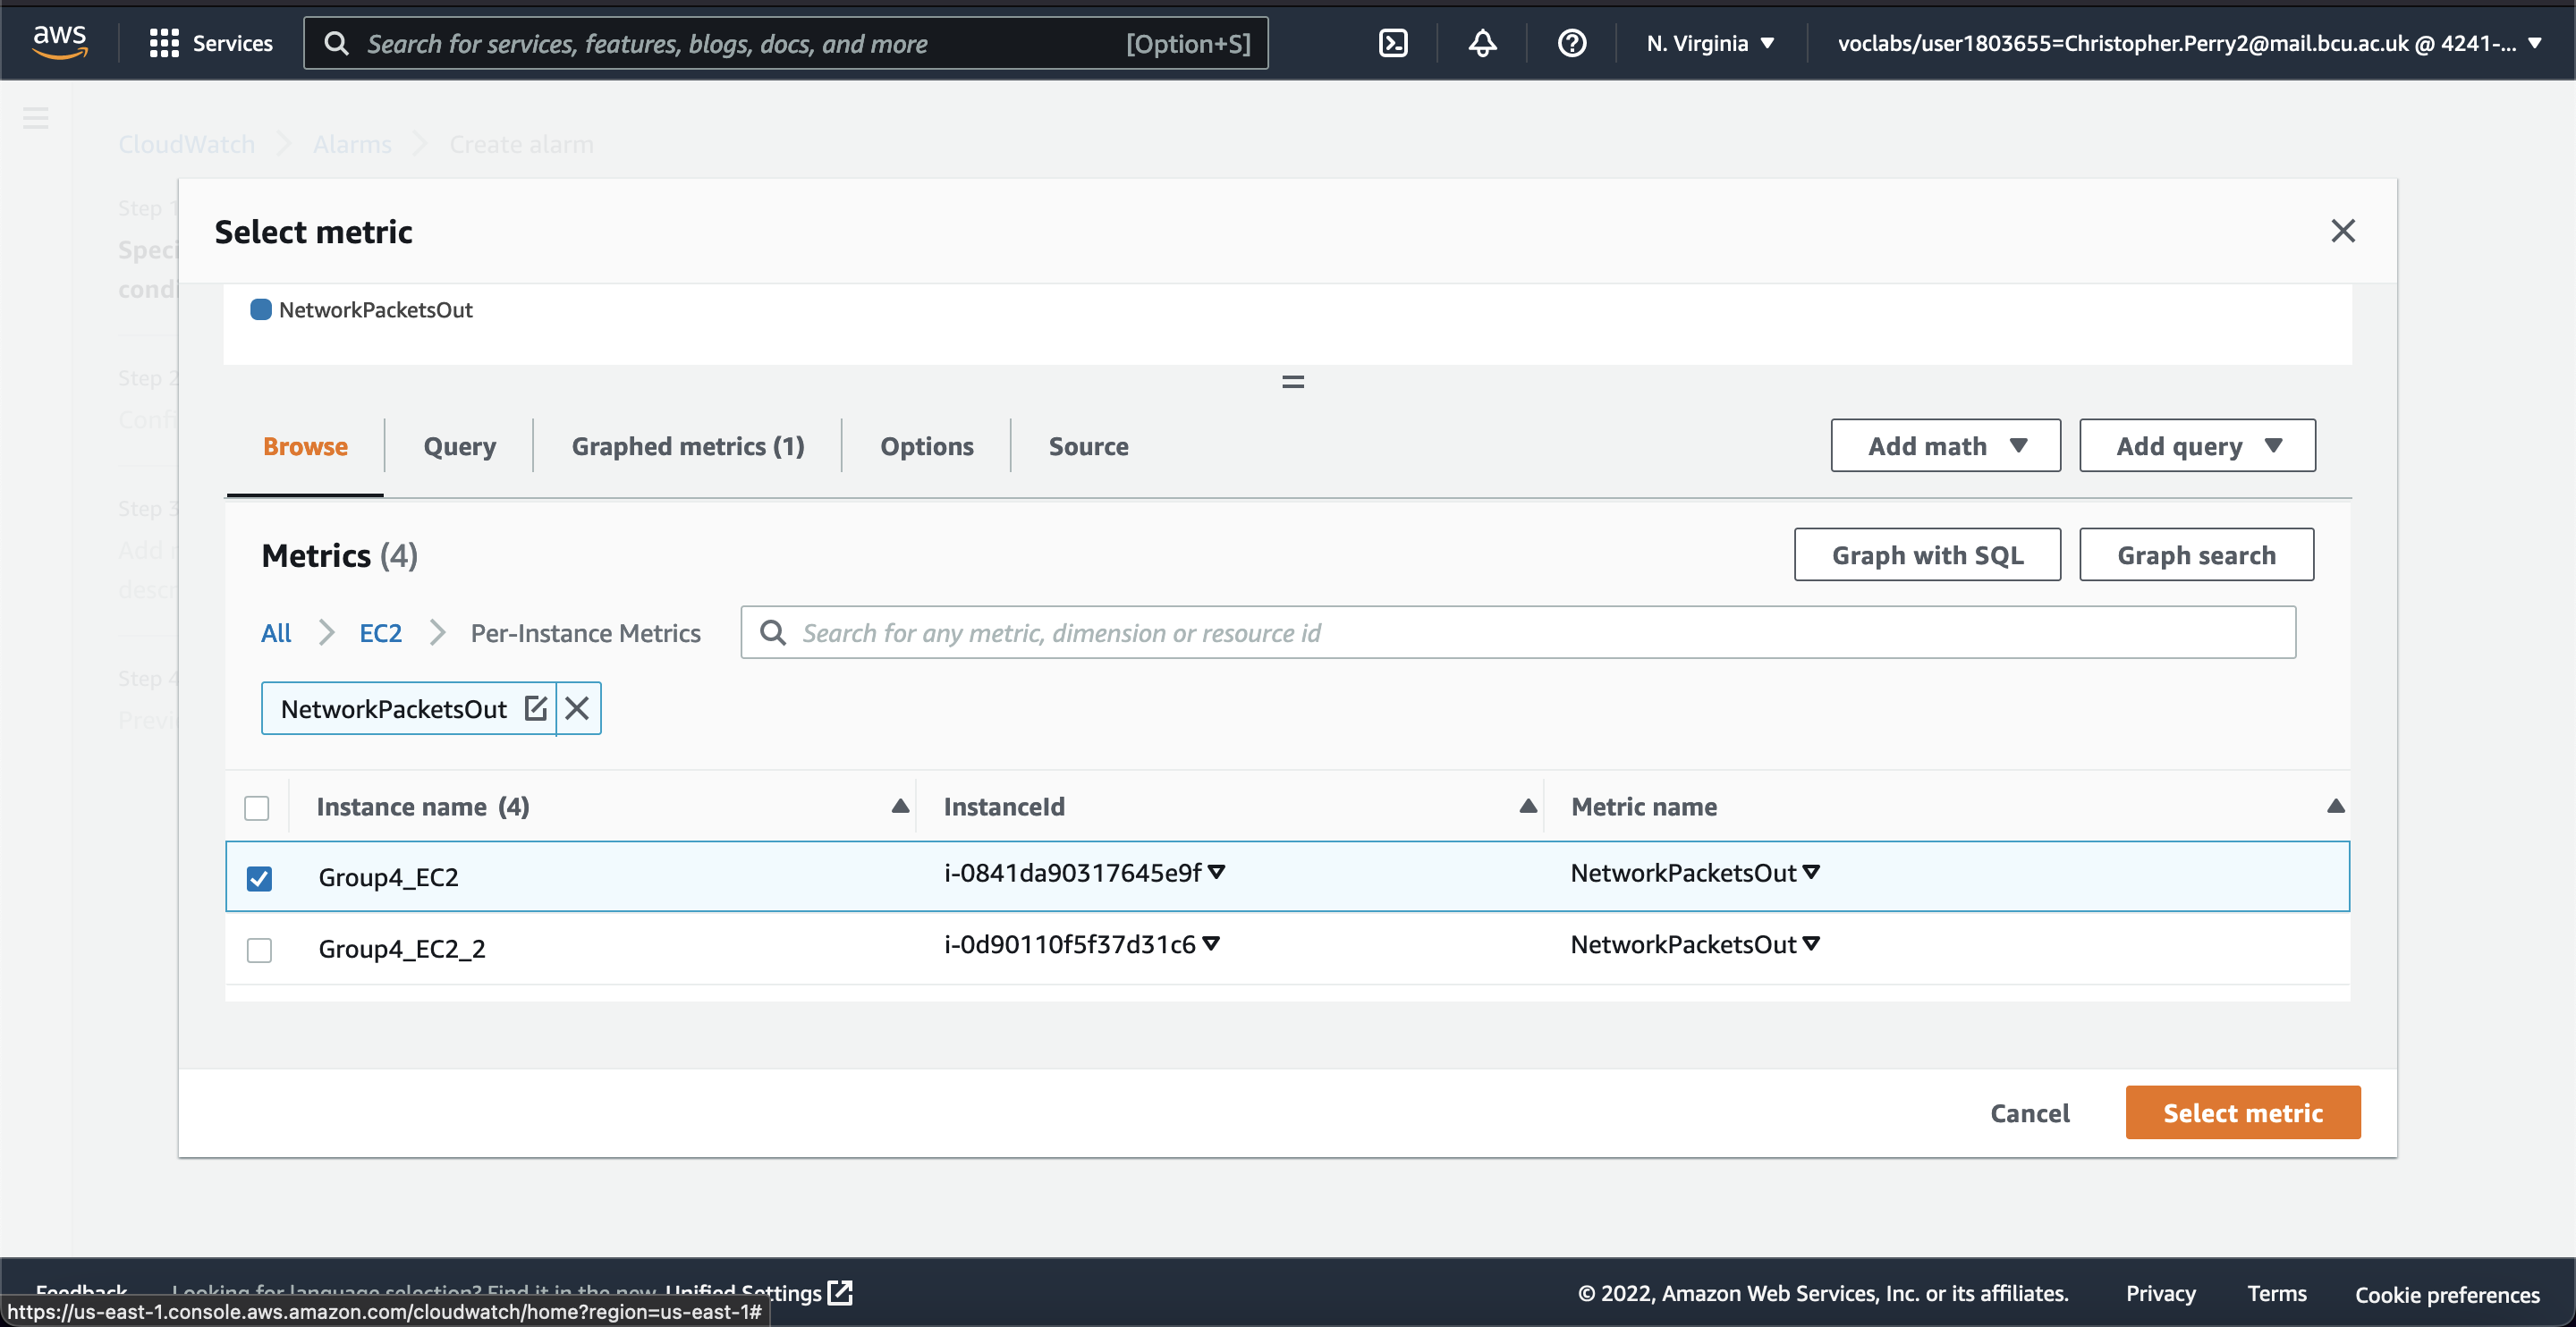
\includegraphics[width=\textwidth]{resources/cloudwatch/cloudwatch-metric-selection}
    \caption{Selection of CloudWatch metric for EC2 instance.}
    \label{fig:cloudwatch-metrics}
\end{figure}

The metric will be configured to alarm in the event that there is less than 5 packets of data sent per day from the
instance.
As the instance currently outputs nearly, 30,000 packets per day, this will be useful to check if the web app has failed.

\begin{figure}[!htbp]
    \centering
    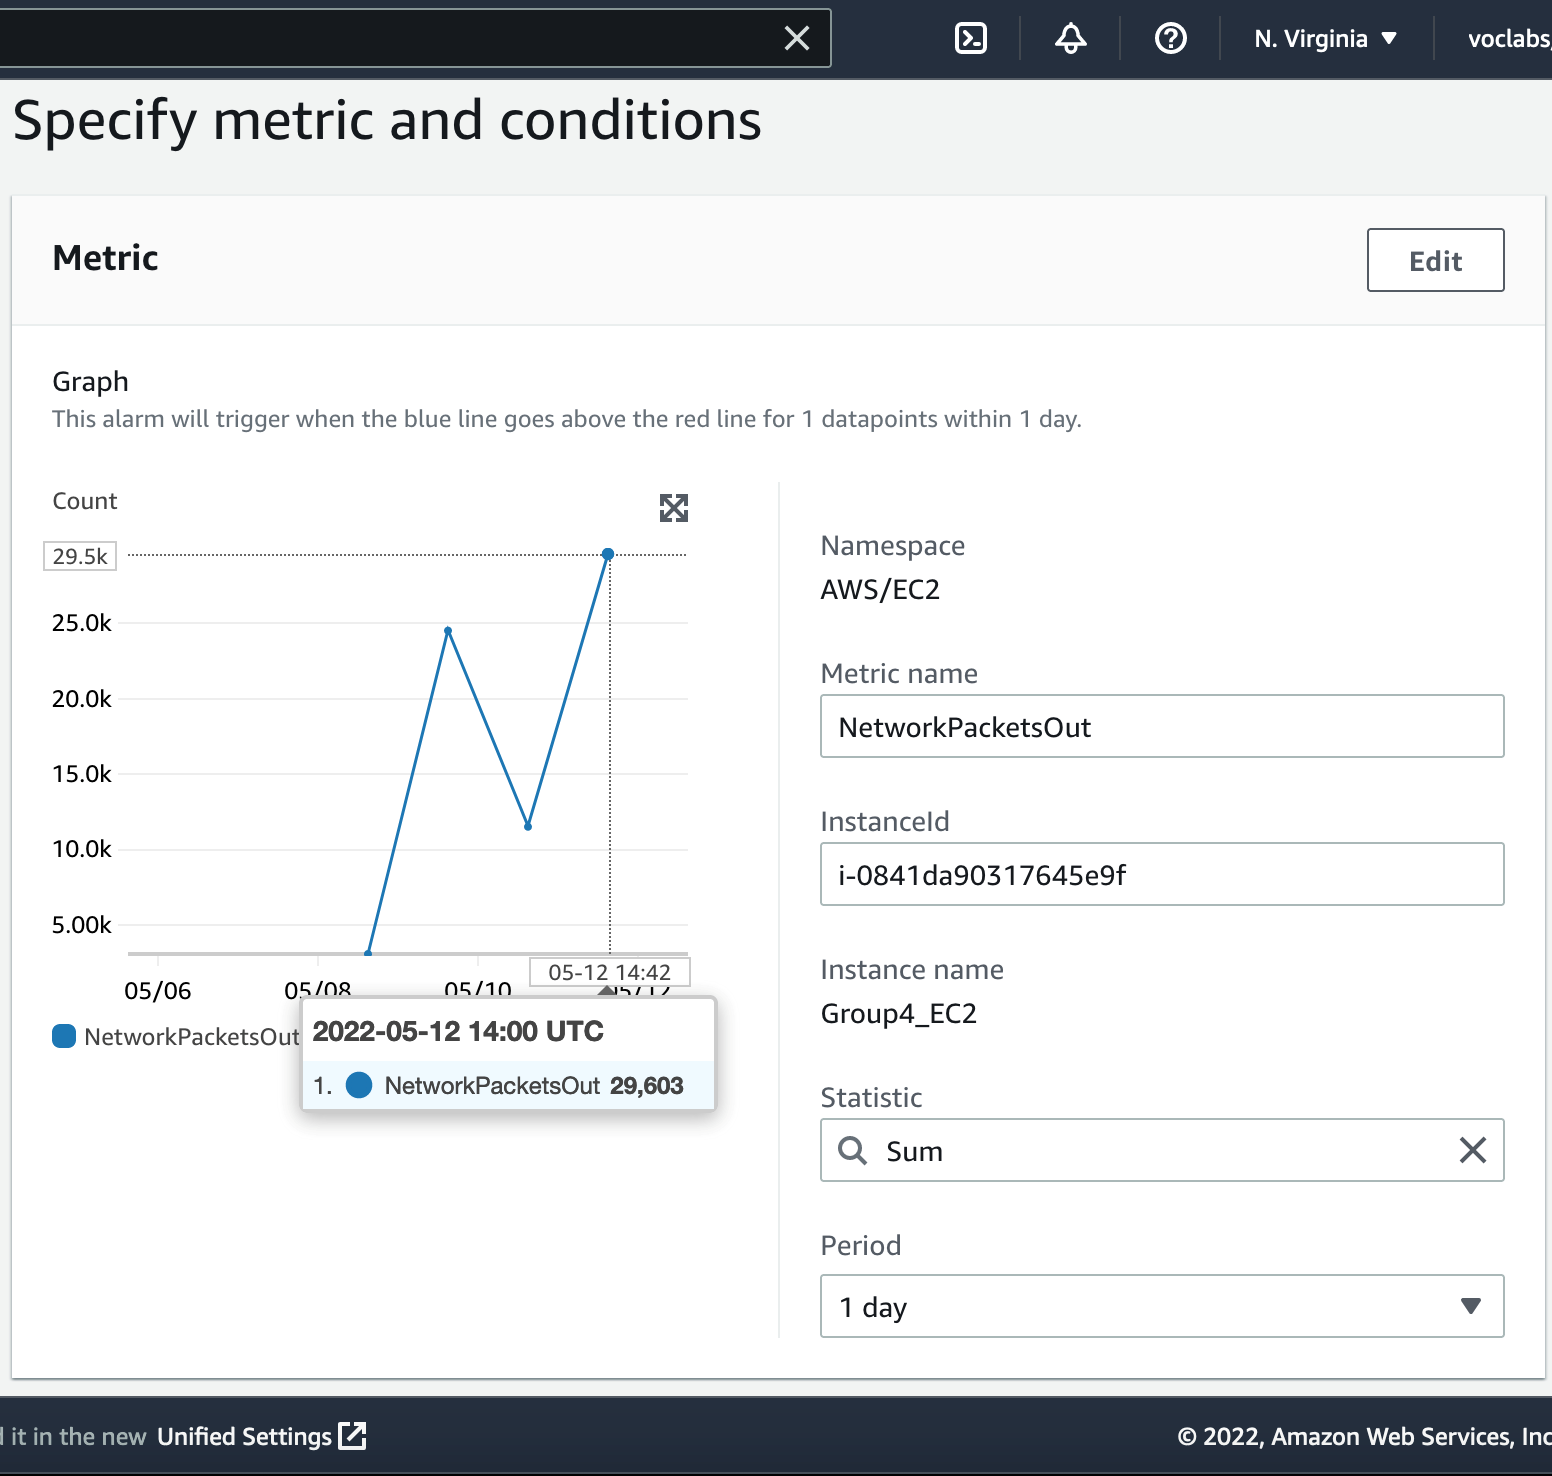
\includegraphics[width=\textwidth]{resources/cloudwatch/cloudwatch-metric-config-1}
    \caption{Configuration of NetworkPacketsOut Metric.}
    \label{fig:cloudwatch-metrics-config-1}
\end{figure}

\begin{figure}[!htbp]
    \centering
    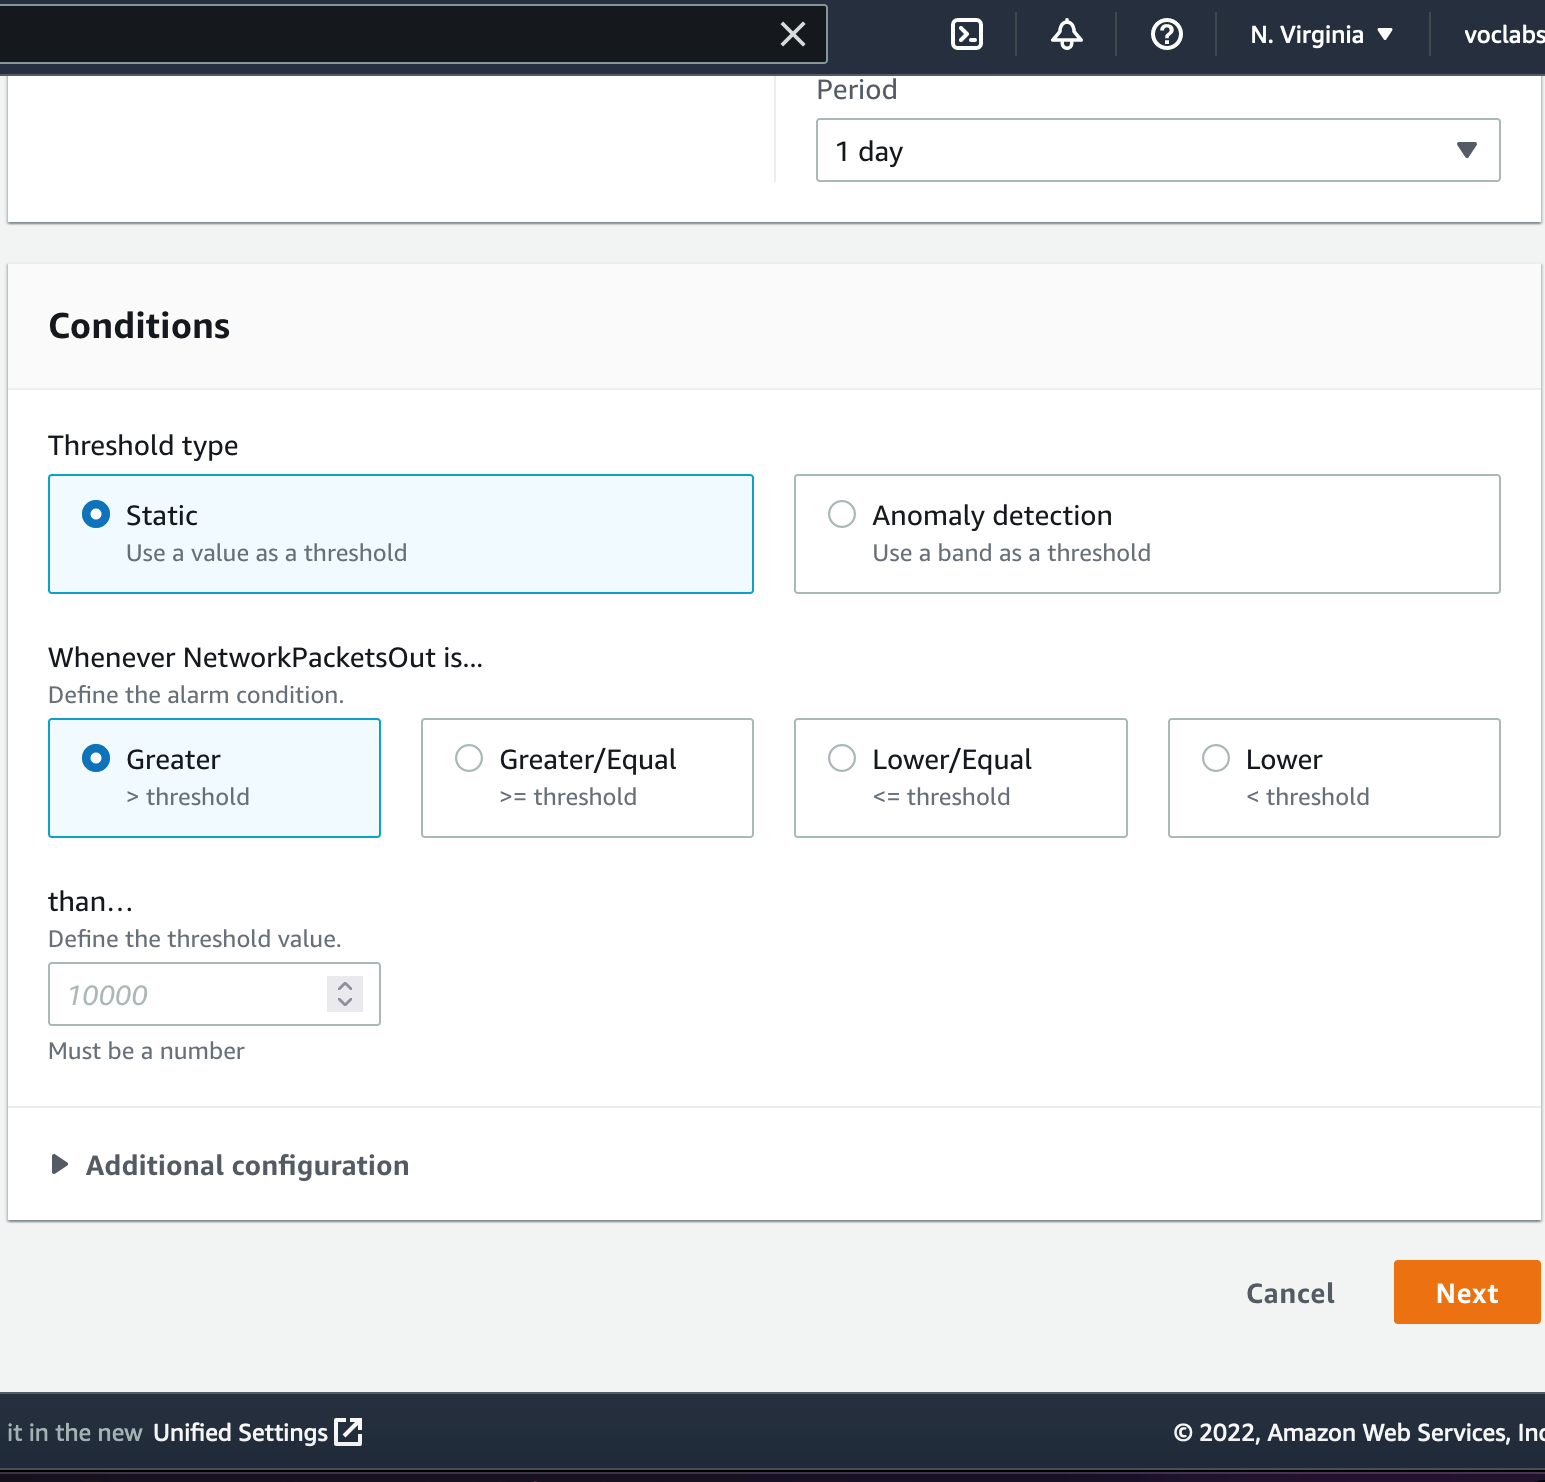
\includegraphics[width=\textwidth]{resources/cloudwatch/cloudwatch-metric-config-2}
    \caption{Configuration of NetworkPacketsOut Metric.}
    \label{fig:cloudwatch-metric-config-2}
\end{figure}

Figures~\ref{fig:cloudwatch-metrics-config-1} and~\ref{fig:cloudwatch-metric-config-2} detail the alarm being set so that
when the sum of packets sent is less than 5 per day, the alarm will activate.

In addition to the initial configuration of these CloudWatch alarms, SNS topics will also be set up so that every member
of the group will be emailed in the event that the alarms activate.
Figure~\ref{fig:cloudwatch-sns-topic} details this process.

\begin{figure}[!htbp]
    \centering
    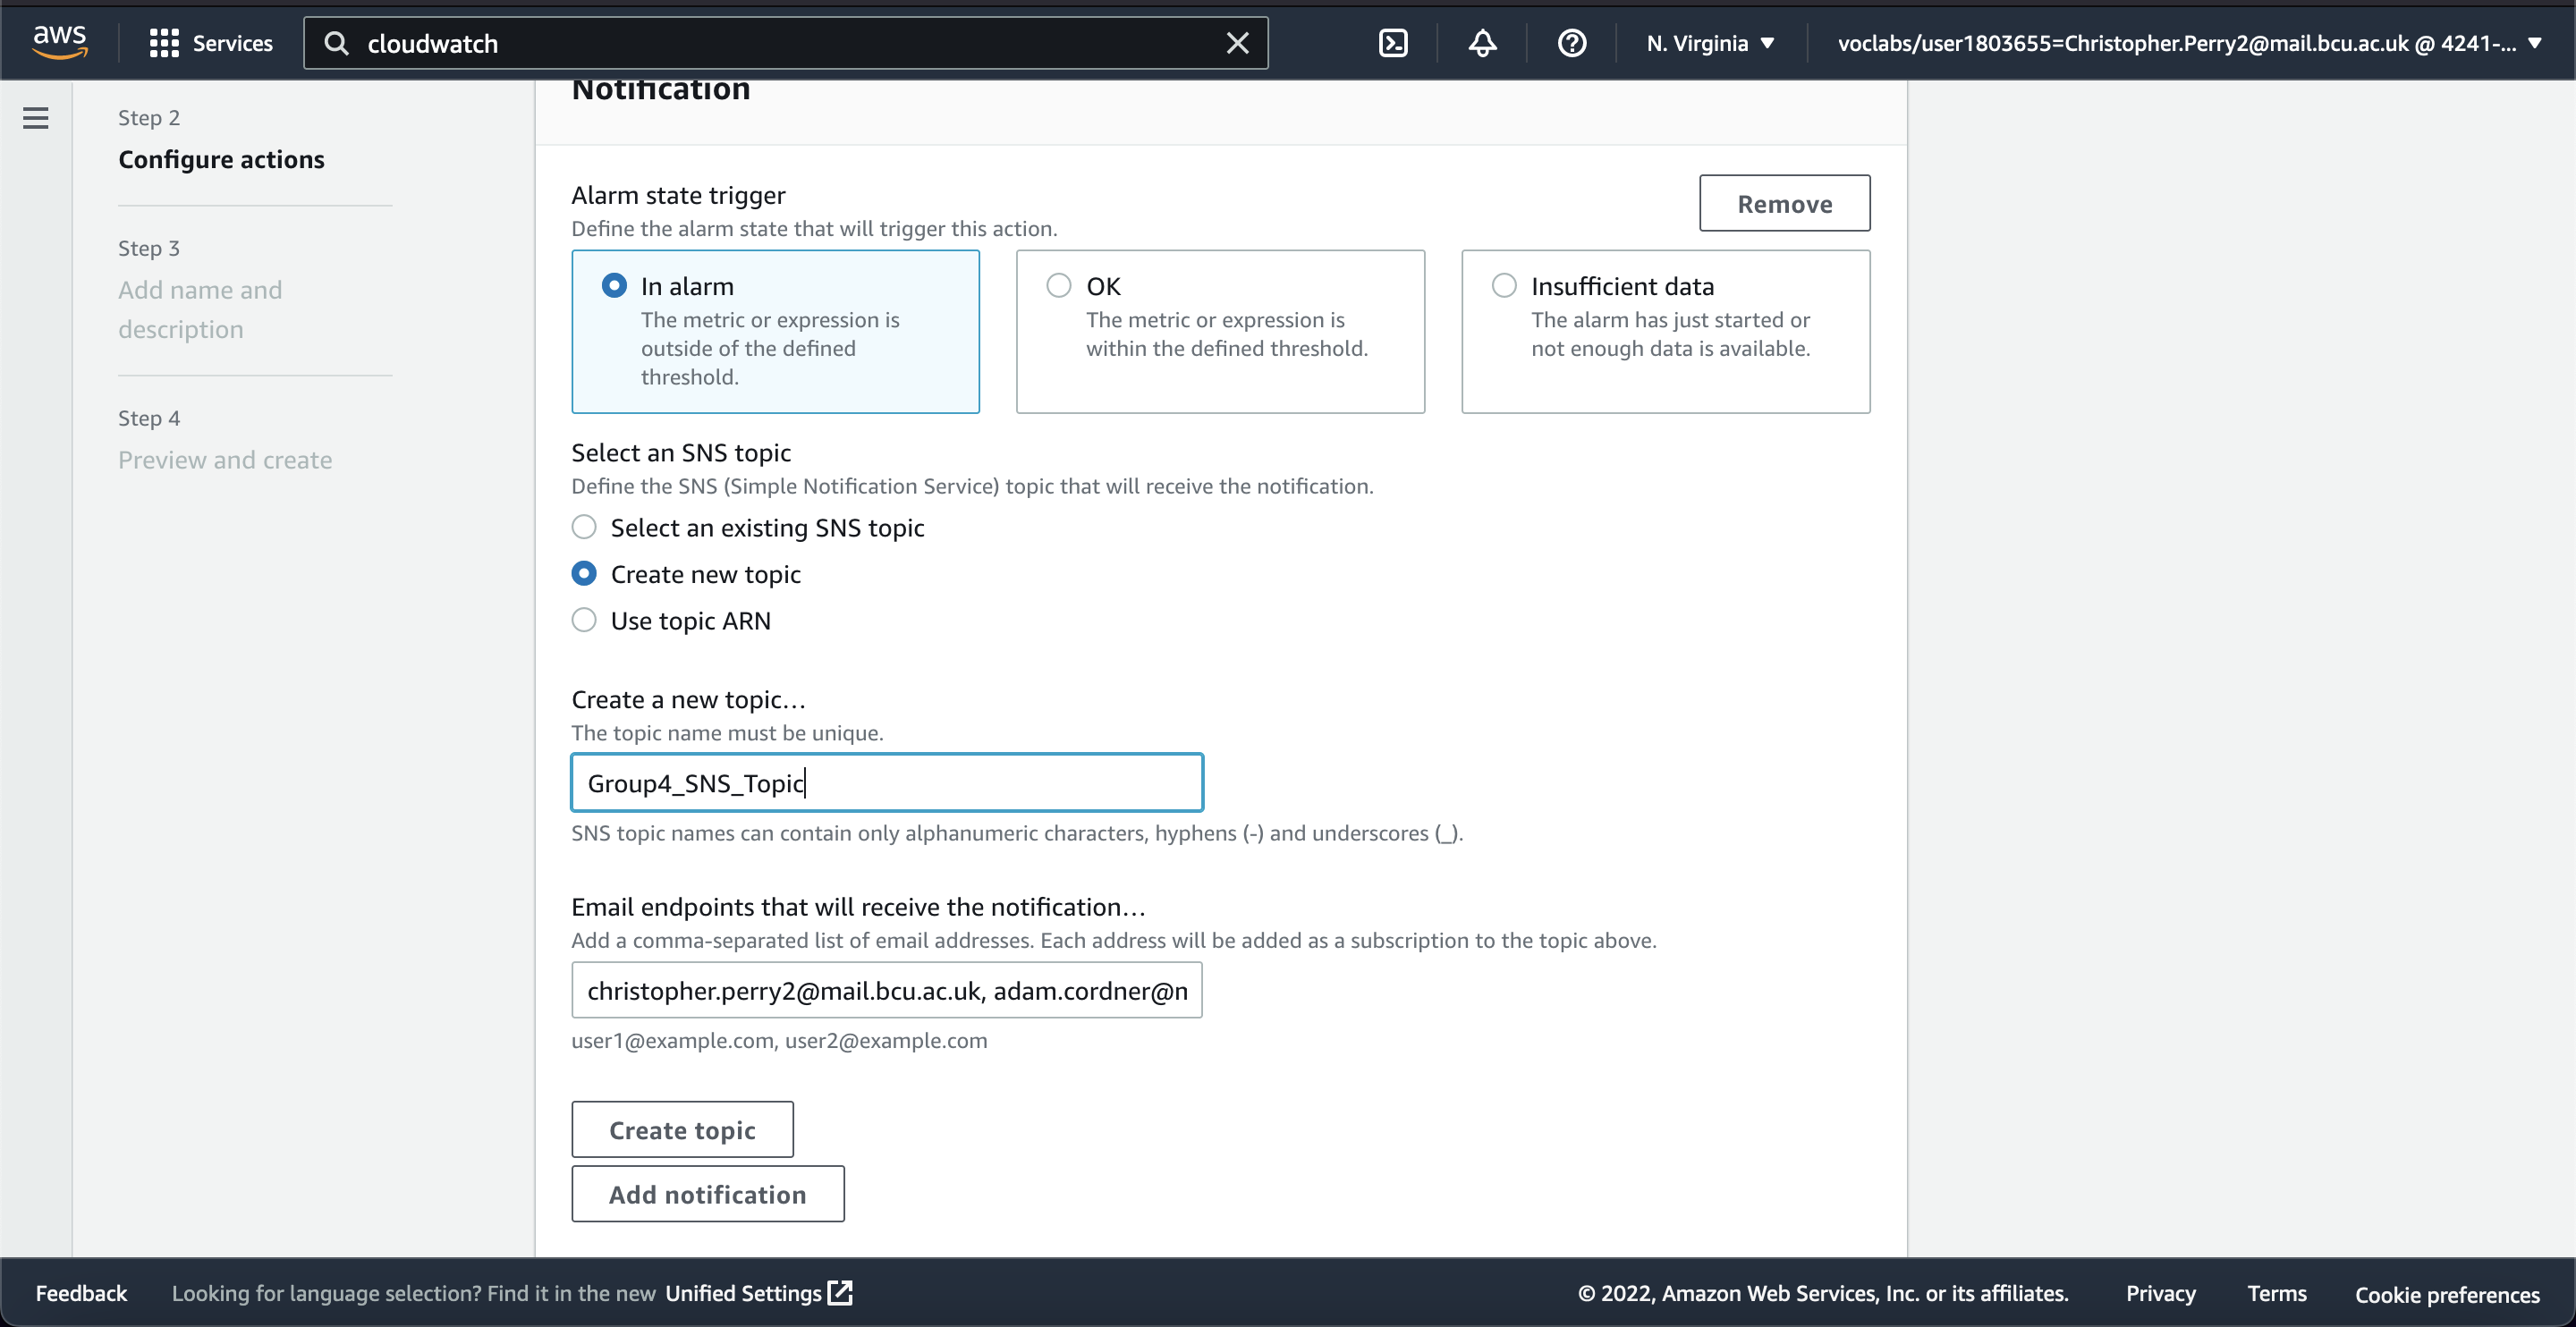
\includegraphics[width=\textwidth]{resources/cloudwatch/cloudwatch-sns-topic}
    \caption{Configuration of SNS Topic for email alerts on alarm activation.}
    \label{fig:cloudwatch-sns-topic}
\end{figure}

An email was then sent to all group members upon completion of this form, and the SNS topic was subsequently subscribed
to, as shown in Figures~\ref{fig:cloudwatch-sns-email} and~\ref{fig:cloudwatch-sns-success}.

\begin{figure}[!htbp]
    \centering
    
\includegraphics[width=\textwidth]{resources/cloudwatch/cloudwatch-email}
    \caption{CloudWatch SNS Topic Email.}
    \label{fig:cloudwatch-sns-email}
\end{figure}

\begin{figure}[!htbp]
    \centering
    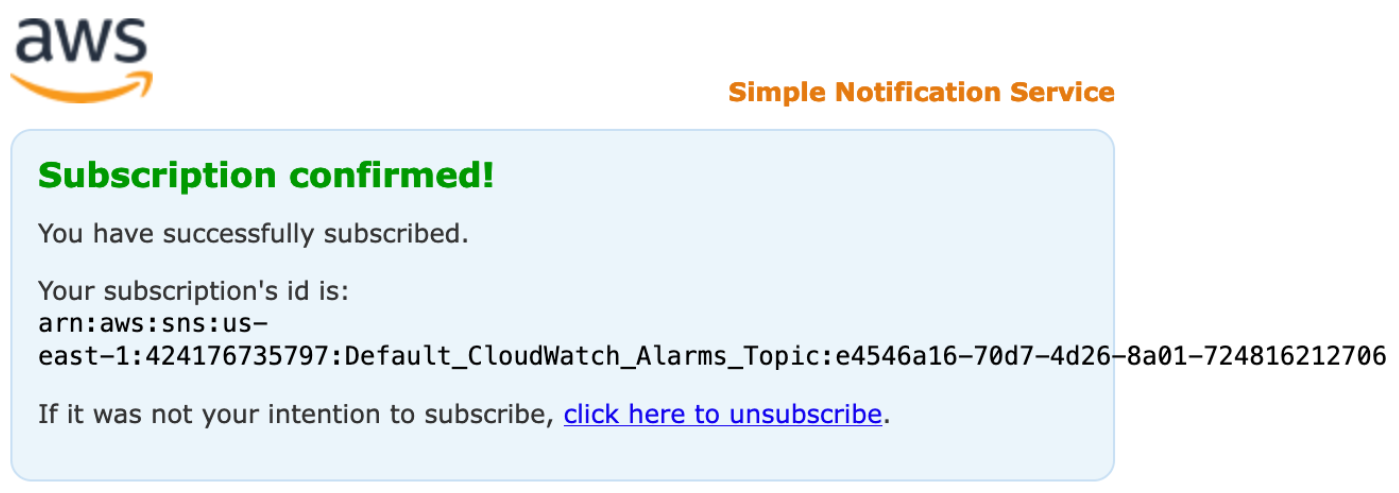
\includegraphics[width=\textwidth]{resources/cloudwatch/cloudwatch-alarm-success}
    \caption{Successful subscription to SNS topic.}
    \label{fig:cloudwatch-sns-success}
\end{figure}

The EC2 instance has also been configured to restart when this alarm activates.
This is done by automatically re-running the scripts used to start the web app on the instance starting up again.

This process can be seen in Figure~\ref{fig:cloudwatch-ec2-actions}.

\begin{figure}[!htbp]
    \centering
    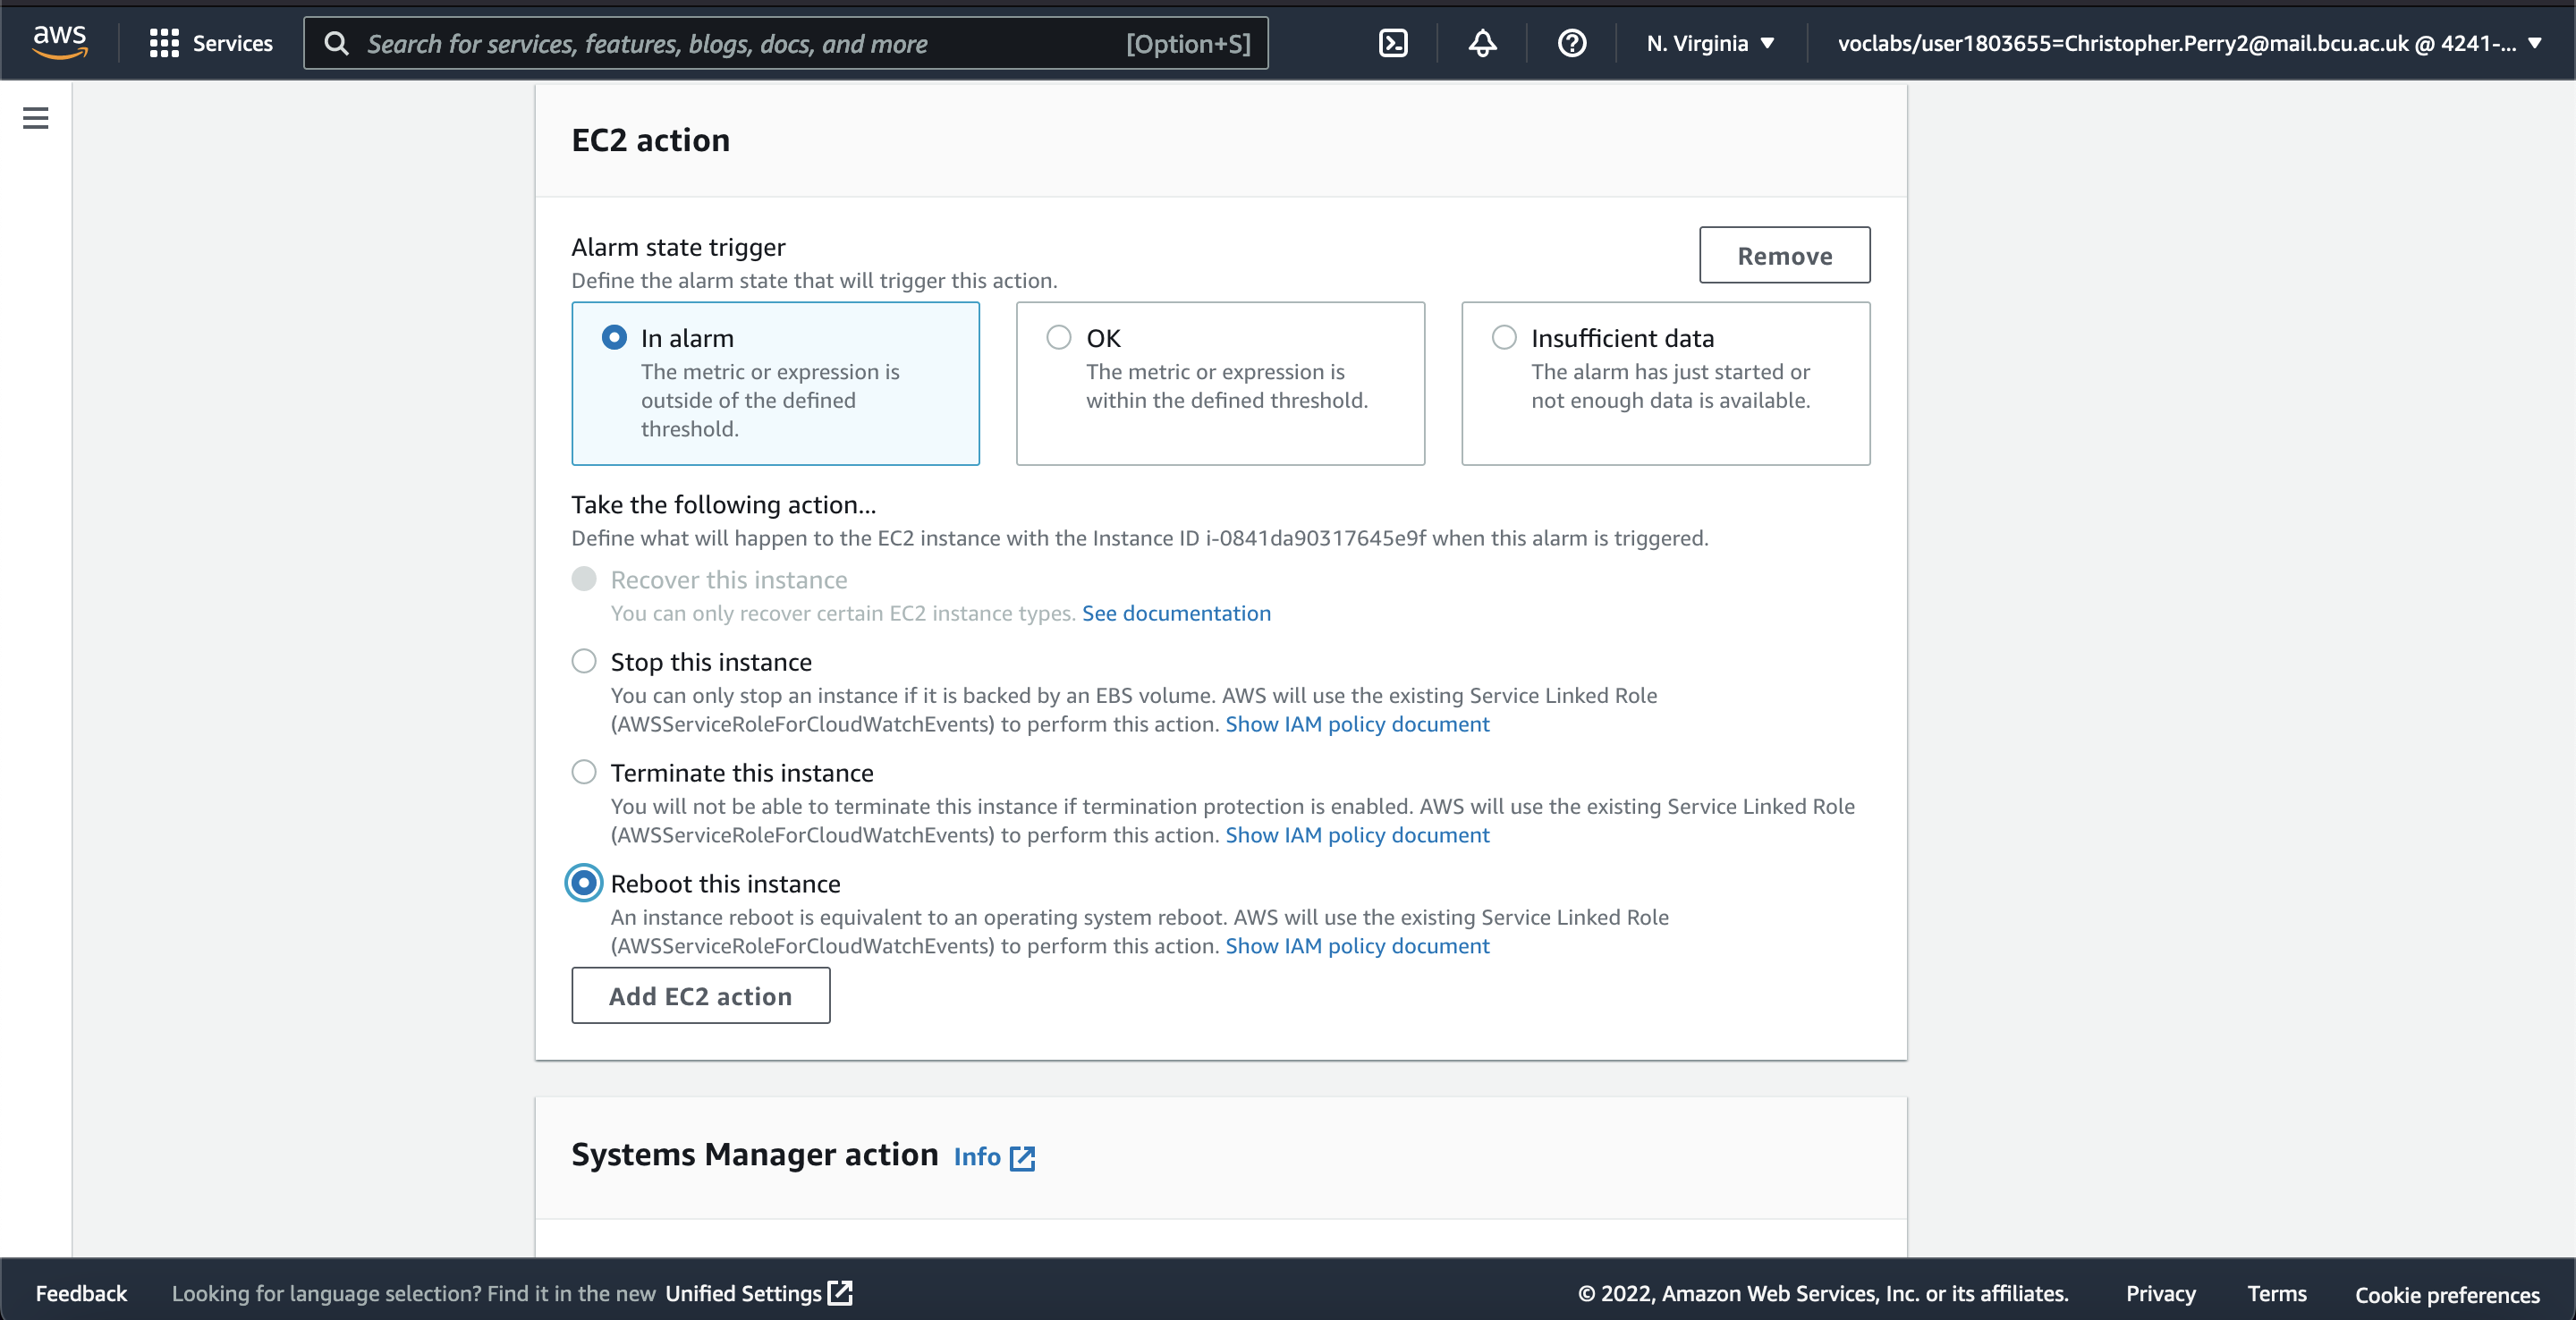
\includegraphics[width=\textwidth]{resources/cloudwatch/cloudwatch-ec2-actions}
    \caption{Configuration for EC2 instance to reboot on alarm activation.}
    \label{fig:cloudwatch-ec2-actions}
\end{figure}

A brief description of the CloudWatch alarm is then added.
This can be seen in Figure~\ref{fig:cloudwatch-description}.

\begin{figure}[!htbp]
    \centering
    \includegraphics[width=\textwidth]{resources/cloudwatch/cloudwatch-description}
    \caption{CloudWatch alarm description.}
    \label{fig:cloudwatch-description}
\end{figure}

The alarm has now been set up, and can be seen in the CloudWatch Management Dashboard in Figure~\ref{fig:cloudwatch-network-alarm}.

\begin{figure}[!htbp]
    \centering
    \includegraphics[width=\textwidth]{resources/cloudwatch/cloudwatch-network-alarm-complete}
    \caption{CloudWatch network alarm in dashboard.}
    \label{fig:cloudwatch-network-alarm}
\end{figure}

In addition to the created network alarm, a charges alarm will also be set up.
A similar process is followed whereby the metric of \mintinline{zsh}|EstimatedCharges| is applied to all
\mintinline{zsh}|AmazonEC2| instances, as detailed in Figure~\ref{fig:cloudwatch-metric-charges}.

\begin{figure}[!htbp]
    \centering
    \includegraphics[width=\textwidth]{resources/cloudwatch/cloudwatch-metric-charges}
    \caption{Selection of \mintinline{zsh}|EstimatedCharges| CloudWatch metric.}
    \label{fig:cloudwatch-metric-charges}
\end{figure}

This metric will be configured to alarm in the event that the EC2 instance uses more than \$15 every 6 hours.
This process can be seen in Figures~\ref{fig:cloudwatch-charges-config-1} and~\ref{fig:cloudwatch-charges-config-2}.

\begin{figure}[!htbp]
    \centering
    \includegraphics[width=\textwidth]{resources/cloudwatch/cloudwatch-charges-config-1}
    \caption{Configuration of CloudWatch alarm.}
    \label{fig:cloudwatch-charges-config-1}
\end{figure}

\begin{figure}[!htbp]
    \centering
    \includegraphics[width=\textwidth]{resources/cloudwatch/cloudwatch-alarm-success}
    \caption{Configuration of CloudWatch alarm.}
    \label{fig:cloudwatch-charges-config-2}
\end{figure}

A brief description was added to the alarm, as seen in Figure~\ref{fig:cloudwatch-charges-description}.

\begin{figure}[!htbp]
    \centering
    \includegraphics[width=\textwidth]{resources/cloudwatch/cloudwatch-charges-description}
    \caption{Description of CloudWatch alarm.}
    \label{fig:cloudwatch-charges-description}
\end{figure}












    \chapter{CloudTrail}\label{ch:cloudtrail}

The use of CloudTrail will allow for logging across the project.
This will give the group control over storage, analysis and any remediation actions.
Visibility of AWS account activity is a recommended AWS security best practice~\parencite{amazon2022cloudtrail}.

CloudTrail will be enabled for any changes which occur within the project's S3 bucket and RDS instances.
The CloudTrail is first given the name of~\mintinline{zsh}|Group4-CloudTrail|.
A location for the logs that CloudTrail outputs is required, so the S3 bucket created in
Chapter~\ref{ch:simple-storage-service} is selected as the storage location.
The "Log file SSE-KMS encryption" option is Enabled, which encrypts the log files that are generated, heightening
security.
A KMS is required to encrypt this data, and a new one is created and named~\mintinline{zsh}|Group4-kms|.
These options can be seen in Figure~\ref{fig:cloudwatch-general-1}.

\begin{figure}[!htbp]
    \centering
    \includegraphics[width=\textwidth]{resources/cloudtrail/cloudtrail-general-1}
    \caption{Initial CloudTrail set up.}
    \label{fig:cloudwatch-general-1}
\end{figure}

\clearpage
The "Log file validation" option is selected, which ensures that any changes which have been to made to the log file
that are not from CloudTrail directly are notified to the group.
These aforementioned notifications have been set up through the creation of new SNS topic
called~\mintinline{zsh}|Group4-cloudtrail-sns|.
These options can be seen in Figure~\ref{fig:cloudwatch-general-2}.

\begin{figure}[!htbp]
    \centering
    \includegraphics[width=\textwidth]{resources/cloudtrail/cloudtrail-general-2}
    \caption{Initial CloudTrail set up.}
    \label{fig:cloudwatch-general-2}
\end{figure}

Now that the CloudTrail initial setup is complete, the selection of the specific events which will be monitored can be
configured.
"Management Events" is firstly selected - this will allow for any read or write events which have been applied on
the S3 and RDS services to be logged.
In addition to this, "Insights Events" is also enabled, which will allow for any unusual activity on these services to
also be logged through the use of the API Call Rate and Error Rate - If they are high, this will be logged via CloudTrail.
which is of a security benefit to the project.
These settings can be seen configured in Figure~\ref{fig:cloudtrail-events}.

\begin{figure}[!htbp]
    \centering
    \begin{minipage}{.5\textwidth}
        \centering
        \includegraphics[width=1\linewidth]{resources/cloudtrail/cloudtrail-events-1}
        \label{fig:cloudtrail-events-1}
    \end{minipage}%
    \begin{minipage}{.5\textwidth}
        \centering
        \includegraphics[width=1\linewidth]{resources/cloudtrail/cloudtrail-events-2}
        \label{fig:cloudtrail-events-2}
    \end{minipage}
    \caption{Configuring CloudTrail events.}
    \label{fig:cloudtrail-events}
\end{figure}

\clearpage
The CloudTrail has now been added and is now monitoring for any activity.
This can be seen in Figure~\ref{fig:cloudtrail-added}.

\begin{figure}[!htbp]
    \centering
    \includegraphics[width=\textwidth]{resources/cloudtrail/cloudtrail-added}
    \caption{Added CloudTrail instance.}
    \label{fig:cloudtrail-added}
\end{figure}

Like with CloudWatch, all users in the SNS topic receive a confirmation email once it has been set up.
This can be seen in Figure~\ref{fig:cloudtrail-validation-message}.

\begin{figure}[!htbp]
    \centering
    \includegraphics[width=\textwidth]{resources/cloudtrail/cloudtrail-validation-message}
    \caption{CloudTrail validation message.}
    \label{fig:cloudtrail-validation-message}
\end{figure}

    \chapter{Relational Database Service (RDS)}\label{ch:relational-database-service}

Amazon RDS is a service which allows developers to create fully-featured and highly-available SQL databases that can be
automatically replicated to additional availability zones.
To create an Amazon RDS instance, a suitable identifier for the database is required before created, as well as a
selection of the resource limits for the virtual server.
The database requires a username and passphrase, although for additional security there is the option to automatically
generate a passphrase.
Afterwards, the type of SQL database required (such as MySQL, PostgreSQL, MariaDB or others) will be selected and then
the database should begin provisioning.

\section{Creation of RDS}\label{sec:creation-of-rds}
Password authentication was used for accessing the RDS instance as the accounts used to develop this deployment were
denied permissions from the root user to create IAM roles within this environment.
In the future, it would be recommended to select one of the other options to improve security, however this was not
possible for the project.

\begin{figure}[!htbp]
    \centering
    \includegraphics[width=\textwidth]{resources/rds/rds-authentication}
    \caption{Selection of RDS authentication options.}
    \label{fig:rds-auth}
\end{figure}

\clearpage
Additionally, an instance with multiple availability zones was selected to ensure that the database was highly
available and that the web app would still be able to access information from the database if one availability
zone becomes unavailable.

\begin{figure}[!htbp]
    \centering
    \includegraphics[width=\textwidth]{resources/rds/rds-availability-durability}
    \caption{Selection RDS multiple availability zones.}
    \label{fig:rds-avail}
\end{figure}

While configuring the RDs instance, it was also required to select a VPC to use.
The VPC created earlier in this deployment was used.
Public access to the database was turned off to further increase security.

\begin{figure}[!htbp]
    \centering
    \includegraphics[width=\textwidth]{resources/rds/rds-connectivity-1}
    \caption{Selection of VPC and subnet groups.}
    \label{fig:rds-connecting}
\end{figure}

\clearpage
Several database engine options are compatible with RDS, including Amazon Aurora, MySQL, MariaDB, and more.
MySQL was chosen for this RDS instance as it is the same database engine used in the local deployment of
\textit{Digital-Ink} within \mintinline{zsh}|docker-compose|.

\begin{figure}[!htbp]
    \centering
    \includegraphics[width=\textwidth]{resources/rds/rds-create-engine}
    \caption{Selection of database engine.}
    \label{fig:rds-engine}
\end{figure}

The database template Dev/Test was selected as it was the cheapest tier that granted support for creating an RDS
instance with multiple availability zones.
The "free tier" provides no support for multiple-AZ deployment.

\begin{figure}[!htbp]
    \centering
    \includegraphics[width=\textwidth]{resources/rds/rds-templates}
    \caption{Selection of database template.}
    \label{fig:rds-templates}
\end{figure}

\clearpage
A micro-sized RDS instance was selected to reduce AWS billing costs where possible.
Figure~\ref{fig:rds-costs} details the estimated RDS cost per month.

\begin{figure}[!htbp]
    \centering
    \includegraphics[width=125mm]{resources/rds/rds-instance-config}
    \caption{Selection of RDS Instance Size.}
    \label{fig:rds-instance-conf}
\end{figure}

\begin{figure}[!htbp]
    \centering
    \includegraphics[width=125mm]{resources/rds/rds-monthly-costs}
    \caption{Estimated Monthly RDS Cost.}
    \label{fig:rds-costs}
\end{figure}

\clearpage
For additional security, a VPC security group is selected for the database.
The previously created security group is selected.
Additionally, RDS login details must be configured.
A master username of \mintinline{zsh}|admin| was chosen, and a password was automatically generated
by AWS with the current best security practices.

\begin{figure}[!htbp]
    \centering
    \includegraphics[width=\textwidth]{resources/rds/rds-security-group}
    \caption{Selection of RDS security group.}
    \label{fig:rds-security}
\end{figure}

\begin{figure}[!htbp]
    \centering
    \includegraphics[width=\textwidth]{resources/rds/rds-settings}
    \caption{Generating credentials for RDS authentication.}
    \label{fig:rds-settings}
\end{figure}

\clearpage
A selection of how much storage the RDS instance is able to access should be made.
It was decided that, due to billing constraints, a small amount of storage, with size to automatically grow if
the application was presented with more users, was most appropriate.

\begin{figure}[!htbp]
    \centering
    \includegraphics[width=125mm]{resources/rds/rds-storage}
    \caption{Selection of Storage Parameters.}
    \label{fig:rds-storage}
\end{figure}

MySQL was selected as it was the same database engine that the web application was originally using within Docker.
The tables were generated using the command \mintinline{zsh}|php artisan migrate|, which generated all of the necessary
tables by using the migration scripts.

\begin{figure}[!htbp]
    \centering
    \includegraphics[width=\textwidth]{resources/rds/rds-tables-creation}
    \caption{Creation of RDS tables.}
    \label{fig:rds-tables}
\end{figure}

\clearpage
\section{Accessing the Database}\label{sec:accessing-the-new-database}
MySQL was installed on the EC2 instance in order to sign in to the new database and create tables.

\begin{figure}[!htbp]
    \centering
    \includegraphics[width=125mm]{resources/rds/rds-mysql-install}
    \caption{Installation of MySQL on the EC2 instance.}
    \label{fig:rds-msql-install}
\end{figure}

MySQL was installed manually on the EC2 instance to provide access to the \mintinline{zsh}|mysql| command,
which allowed for signing into the database.
The command \mintinline{zsh}|mysql -h \$ENDPOINT -u admin -p\$PASSWORD| was then used.

\begin{figure}[!htbp]
    \centering
    \includegraphics[width=125mm]{resources/rds/rds-database-creation}
    \caption{Creation of a database.}
    \label{fig:rds-db-create-2}
\end{figure}

\clearpage
The web application required a database table to be created manually before the database migrations could be run, so
following command was used within the RDS SQL environment: \mintinline{sql}|CREATE DATABASE group4_db;|.

\begin{figure}[!htbp]
    \centering
    \includegraphics[width=125mm]{resources/rds/envupdate}
    \caption{Changing the database endpoint from Docker to AWS RDS.}
    \label{fig:rds-env-update}
\end{figure}

After the database was set up, tested and working, the old MySQL docker container was removed from the docker-compose
file.

\begin{figure}[!htbp]
    \centering
    \includegraphics[width=50mm]{resources/rds/docker}
    \caption{Removal of database from docker file.}
    \label{fig:rds-rm-docker-compose}
\end{figure}

As old database was no longer needed within the \mintinline{zsh}|docker-compose.yml| file, the container was removed and
only Amazon RDS was used.

    \chapter{Elastic Load Balancing (ELB)}\label{ch:elastic-load-balancing}

Elastic Load Balancing is used to automatically scale your EC2 instances to meet any changes in demand from your users.
ELB can be used to both scale up or down the instance's resources to ensure that your application is kept performant and
available regardless of how many users visit.
It is also possible to scale down the resources again, after the spike in usage has passed, to save money when it comes
to billing and ensure you aren't paying for any additional resources that are not being used.

\section{Step 1: Creation of new AMI}

\begin{enumerate}
	\item Selection of AMI previously created and then "Create Instance from AMI" option \begin{figure}[H]
	      \centering
	      \includegraphics[width=\textwidth]{resources/elb/elb-instance-from-ami.png}
	      \caption{Creation of Instance from AMI Image}
	      \label{fig:elb-instance-from-ami}
	\end{figure}
	\item AMI selected to use same instance as "Group4-EC2" so everything is the same \begin{figure}[H]
	      \centering
	      \includegraphics[width=\textwidth]{resources/elb/elb-instance-2-name.png}
	      \caption{Naming Second Instance}
	      \label{fig:elb-instance-2-name}
	\end{figure}
	\item Same keypair used, so it is easier to switch between both instances \begin{figure}[H]
	      \centering
	      \includegraphics[width=\textwidth]{resources/elb/elb-instance-2-type-and-keypair.png}
	      \caption{Selection of Keypair \& Instance Size}
	      \label{fig:elb-type-and-keypair}
	\end{figure}
	Network Settings
	\item VPC set to be Group4 VPC  (created in Section~\ref{ch:vpc})
	\item Subnet set to be "Public Subnet 2"
	\item Public IP auto-assigned
	\item Existing security group of "Group4-Security-Group" selected to allow HTTP, HTTPS, SSH and MySQL traffic on the
	      instance \begin{figure}[H]
	      \centering
	      \includegraphics[width=\textwidth]{resources/elb/elb-instance-2-network-settings.png}
	      \caption{Selection of VPC and Security Group}
	      \label{fig:elb-instance-2-network-setting}
	\end{figure}
	\item Storage remains the same as previous instance

	      \begin{figure}[H]
	      	\centering
	      	\includegraphics[width=\textwidth]{resources/elb/elb-instance-2-storage-config.png}
	      	\caption{Selection of Instance Storage Size}
	      	\label{fig:elb-instance-2-storage}
	      \end{figure}
	\item Second instance now created \begin{figure}[H]
	      \centering
	      \includegraphics[width=\textwidth]{resources/elb/elb-instance-2-created.png}
	      \caption{Second Instance Creation Success}
	      \label{fig:elb-instance-2-create}
	\end{figure}
\end{enumerate}

\section{Step 2: Creation of target group}

Now that there are 2 instances, they both need to be stored within a target group.

\begin{enumerate}
	\item The Target Group type of "Instances" is selected - this will store both running instances of Digital-Ink in a group
	      to be handled by the Load Balancer
	\item Target Group name of "Group4-Target-Group" given
	\item Protocol of HTTP and port 80 given \begin{figure}[H]
												 \centering
												 \includegraphics[width=\textwidth]{resources/elb/elb-target-group-basic-config.png}
												 \caption{Setting Target Type, Protocol \& Port}
												 \label{fig:elb-target-group-basic-config}
	\end{figure}
	\item Group4-VPC selected \begin{figure}[H]
	      \centering
	      \includegraphics[width=\textwidth]{resources/elb/elb-vpc.png}
	      \caption{Selection of Group 4 VPC}
	      \label{fig:elb-vpc}
	\end{figure}
	\item The next screen asks for instances that will be registered to the Target Group to be selected
	\item The 2 running instances of Digital Ink are shown and added as targets through the "Include as pending below"
	      button \begin{figure}[H]
	      \centering
	      \includegraphics[width=\textwidth]{resources/elb/elb-register-targets.png}
	      \caption{Include as Pending Below}
	      \label{fig:elb-register-targets}
	\end{figure}
	\item Target group now created, and contains both EC2 instances within them \begin{figure}[H]
	      \centering
	      \includegraphics[width=\textwidth]{resources/elb/elb-target-group-created.png}
	      \caption{Target Groups Success}
	      \label{fig:elb-target-group-create}
	\end{figure}
\end{enumerate}

\section{Step 3: Creation of Load Balancer}

\begin{enumerate}
	\item The Target groups are not associated with a Load Balancer, so one will be created as an Application Load Balancer
	      \begin{figure}[H]
	      	\centering
	      	\includegraphics[width=\textwidth]{resources/elb/elb-load-balancer-creation.png}
	      	\caption{No Load Balancer Configured Warning}
	      	\label{fig:elb-load-bal-create}
	      \end{figure}
	\item Given the name of "Group4-Load-Balancer' \begin{figure}[H]
													   \centering
													   \includegraphics[width=\textwidth]{resources/elb/elb-basic-config.png}
													   \caption{Load Balancer Creation}
													   \label{fig:elb-creation-config}
	\end{figure}
	\item Set to be internet facing and will handle IPv4 addresses \begin{figure}[H]
	      \centering
	      \includegraphics[width=\textwidth]{resources/elb/elb-network-mapping.png}
	      \caption{Load Balancer Network Mapping}
	      \label{fig:elb-networ-mapping}
	\end{figure}
	\item The security group of Group4-Security-Group is selected, which allows HTTP, HTTPS, SSH and MySQL traffic within
	      the load balancer
	\item In the event that either of the web apps goes down, it will be forwarded to the Group4-Target-Group, which will then
	      display the available instance \begin{figure}[H]
	      \centering
	      \includegraphics[width=\textwidth]{resources/elb/elb-security-groups-and-listeners.png}
	      \caption{Listeners and Routing Configuration}
	      \label{fig:elb-security-groups}
	\end{figure}
	\item Could not create Global Accelerator due to permissions issue (Future improvement, please see Chapter~\ref{ch:future-enhancements})
	      \begin{figure}[H]
	      	\centering
	      	\includegraphics[width=\textwidth]{resources/elb/elb-accelerator.png}
	      	\caption{There Was a Problem Creating Global Accelerator}
	      	\label{fig:elb-accelerators}
	      \end{figure}
	\item Summary

	      \begin{figure}[H]
	      	\centering
	      	\includegraphics[width=\textwidth]{resources/elb/elb-summary.png}
	      	\caption{Final Load Balancing Summary}
	      	\label{fig:elb-summary}
	      \end{figure}


	\item Load balancer created
	      \begin{figure}[H]
	      	\centering
	      	\includegraphics[width=\textwidth]{resources/elb/elb-created.png}
	      	\caption{Load Balancer List View}
	      	\label{fig:elb-created}
	      \end{figure}

	\item When the load balancer is visited at
	      \href{http://http://group4-load-balancer-1914525647.us-east-1.elb.amazonaws.com/}{http://http://group4-load-balancer-1914525647.us-east-1.elb.amazonaws.com/},
	      the website is shown
	      \begin{figure}[H]
	      	\centering
	      	\includegraphics[width=\textwidth]{resources/elb/elb-working.png}
	      	\caption{Load Balancer Basic Functionality Test}
	      	\label{fig:elb-working}
	      \end{figure}
\end{enumerate}

\section{Step 4: In-Depth Testing of Load Balancer}

By stopping individual instances, we are able to test the functionality of the load balancer to ensure that it is functioning correctly. When one instance goes down, the other instance should automatically respond to further requests to ensure application's service is not affected.

\begin{figure}[H]
	\centering
	\includegraphics[width=\textwidth]{resources/elb/elb-test-stopped-instance.png}
	\caption{Elastic Load Balancing}
	\label{fig:elb-stopped-instance}
\end{figure}
\begin{figure}[H]
	\centering
	\includegraphics[width=\textwidth]{resources/elb/elb-test-stopped-instance-2.png}
	\caption{Elastic Load Balancing}
	\label{fig:elb-stopped-instance-2}
\end{figure}
    \chapter{Security Practices}\label{ch:security-practices}
AWS provides a variety of services and tools which can be configured to ensure a high level of security within the
cloud architecture used for the deployment.
Cyber security is a vital aspect of any online service as it is important to protect the resources hosted on AWS from
cyberattacks and to prevent the web app itself from being taken off the web~\parencite{cavelty2010cyber}.
It is critical that the best security practices are followed to ensure a high level of security.
This chapter will detail the security measures taken during the deployment of the AWS architecture.

When configuring EC2, a KeyPair was set up for logging into the instance.
This KeyPair is stored on a secure \mintinline{zsh}|.pem| file which should only be accessible to those who created
the EC2 instance.
The KeyPair is required to log into the instance and, therefore, only the authorised users who are part of the
development team have access to editing the EC2 instance.

\begin{figure}[!htbp]
    \centering
    \begin{minipage}{.5\textwidth}
        \centering
        \centering
        \includegraphics[width=1\linewidth]{resources/ec2/create-key-pair-2}
        \label{fig:create-keypair-pem}
    \end{minipage}%
    \begin{minipage}{.5\textwidth}
        \centering
        \includegraphics[width=1\linewidth]{resources/log-in-with-key-pair-2}
        \label{fig:log-in-keypair-pem}
    \end{minipage}
    \caption{Creating and using the KeyPair.}
    \label{fig:create-use-keypair}
\end{figure}

\clearpage
EC2 security groups are virtual firewalls used to control incoming and outgoing traffic for the AWS
deployment~\parencite{amazon2022amazon2}.
Security groups were implemented which limit connections to HTTP, HTTPS, SSH, and MySQL\@.
The HTTP, HTTPS, and MySQL connections were made accessible by public IP addresses as all users who access the web app
would require these permissions (HTTP and HTTPS to view the web app, and MySQL to query the database through the web
app).
The SSH connections are limited to one IP address (eduroam) as the public does not need access.
In a future deployment, the IP address with permission to access the SSH would be set to a private location, such as an
office, rather than eduroam.
During this deployment, the IP address of eduroam was allowed access due to the location in which the deployment was
configured.

\begin{figure}[!htbp]
    \centering
    \subfloat{\includegraphics[width=\textwidth]{resources/security/security-group-name}}\hfill
    \subfloat{\includegraphics[width=\textwidth]{resources/security/security-group-rules}}\hfill
    \subfloat{\includegraphics[width=\textwidth]{resources/security/security-group-created}}\hfill
    \subfloat{\includegraphics[width=\textwidth]{resources/security/security-group-associated}}
    \caption{Configuring security group.}
    \label{fig:security-groups}
\end{figure}

IAM is an AWS service which provides fine-tuned access control across the entire AWS deployment by creating a policy
which specifies which users have permission to access certain features and resources~\parencite{amazon2022aws2}.
Ideally, this would be implemented for security purposes.
Unfortunately, this feature could not be used due to restricted permissions.

\begin{figure}[!htbp]
    \centering
    \includegraphics[width=\textwidth]{resources/iam-denied}
    \caption{Restricted permissions preventing the creation of IAM roles.}
    \label{fig:iam-denied}
\end{figure}

The S3 bucket was configured to use server-side encryption to safely store the data in the bucket.
This was done by specifying to use an Amazon S3-managed key (SSE-S3), i.e. an encryption key which Amazon S3
automatically creates, manages, and uses to encrypt the data.

\begin{figure}[!htbp]
    \centering
    \includegraphics[width=\textwidth]{resources/s3_encryption}
    \caption{S3 bucket encryption settings.}
    \label{fig:s3-encryption}
\end{figure}

When setting up the RDS for the web app, database authentication was configured to require password authentication.
This means that direct access to the SQL database requires the use of a master username and a master password generated
by AWS.
The process of configuring this can be seen in Figure x.

\begin{figure}[!htbp]
    \centering
    \includegraphics[width=\textwidth]{resources/rds_authentication}
    \caption{Setting up database authentication.}
    \label{fig:setup-rds-auth}
\end{figure}

\begin{figure}[!htbp]
    \centering
    \includegraphics[width=\textwidth]{resources/RDS_password}
    \caption{Viewing log in details for database authentication.}
    \label{fig:view-rds-auth}
\end{figure}

%S3 bucket isn't publicly accessible from the get-go
%If we do need public access, it is ONLY for GET or PUT requests (Viewing stories and uploading them)
%
%VPC controlling inbound and outbound traffic
%
%public and private subnets
%
%\begin{figure}[!htbp]
%    \centering
%    \includegraphics[width=\textwidth]{resources/rds/rds-connectivity-1}
%    \caption{Selection of VPC and Subnet Groups.}
%    \label{fig:rds-connect-2}
%\end{figure}
%
%Public access was turned off to further increase our application's security.
%
%\begin{figure}
%    \centering
%    \includegraphics[width=\textwidth]{resources/rds/rds-settings}
%    \caption{Credentials for RDS Authentication.}
%    \label{fig:rds-settings-2}
%\end{figure}
%
%We selected an automatically generated password to ensure that it was created with current best security practices.
    \chapter{Cost Breakdown}\label{ch:cost-breakdown}

If we wished to deploy this web app to the public, or to expand it to a larger market, it would be important to
gather estimated costs for hosting the app in the cloud with all the AWS services being used.
We can use the AWS Pricing Calculator to calculate current costs and predict future costs.
To calculate these costs, it is required to specify every implemented feature and several projected inputs and outputs,
such as amount of data transferred on the app per month.
We began by calculating a monthly cost and a yearly cost of deploying the app in its current state.
Following this, we used the calculator to predict monthly a

In order to predict costs for the use of the AWS infrastructure, estimates from the official AWS
calculator were utilized. The AWS calculator required every implemented feature to be
inserted, as well as the projected inputs/outputs. E.g. how much data is transferred in a month.
The predicted monthly costs and yearly costs were output by the calculator given the present
state of the application on AWS. Following the initial prediction obtained from the AWS
calculator, those figures were used to create other scenarios for if the application gained 1000
to 10000000 users. The figures are used to estimate the costs when the application is scaled
up.


\section{Estimated Costs}\label{sec:estimated-costs}


\section{Scaling Up to 10,000 Users}\label{sec:scaling-up-to-10000-users}


\section{Scaling Up to 1 Million Users}\label{sec:scaling-up-to-1-million-users}


\section{Scaling Up to 10 Million Users}\label{sec:scaling-up-to-10-million-users}

    \chapter{Testing}\label{ch:testing}

This chapter of the report will detail the testing conducted on the configured AWS services.
This was done to determine the accuracy and efficiency of the configurations made during the deployment process.
The testing was conducted by using Gherkin, a language used to define behaviour and test
cases~\parencite{dos2018automated}.
It is non-technical and is intended to be easily human-readable.
Gherkin uses set keywords for structure and meaning: Given, When, and Then.
An example of this structure can be seen in Figure~\ref{fig:gherkin}.

\begin{figure}[!htbp]
    \centering
    \begin{minted}{cucumber}
    Scenario: ...
        Given ...
        When ...
        Then ...
    \end{minted}
    \label{fig:gherkin}
\end{figure}

EC2, S3, CloudFront, RDS, CloudWatch, and CloudTrail were all tested using this approach.
Screenshots are included to illustrate the results of these tests.

\section{Testing EC2}\label{sec:testing-ec2}

\begin{figure}[!htbp]
    \centering
    \begin{minted}{cucumber}
Scenario: Accessing instance through SSH with .pem file private key.
    Given that the EC2 instance is running on AWS and the user has EC2 keypair
    When the user enters the command
    "ssh -i Group4_KeyPair.pem ec2-user@52.45.13.111" in the terminal
    Then the user will be logged into the EC2 instance
    \end{minted}
    \label{fig:accessing-instance-ec2}
\end{figure}

\begin{figure}[!htbp]
    \centering
    \includegraphics[width=\textwidth]{resources/ec2/ec2-logged-in}
    \label{fig:ec2-test-logged-in}
\end{figure}

\clearpage

\begin{figure}[!htbp]
    \centering
    \begin{minted}{cucumber}
Scenario: Accessing web app through EC2 domain name.
    Given that the web app is running on the EC2 instance
    When the user accesses
    "http://ec2-52-45-13-111.compute-1.amazonaws.com" in their browser
    Then the web app will be loaded
    \end{minted}
    \label{fig:accessing-web-app-ec2}
\end{figure}

\begin{figure}[!htbp]
    \centering
    \includegraphics[width=\textwidth]{resources/ec2/digital-ink-ec2}
    \label{fig:ec2-test-digital-ink}
\end{figure}

\clearpage

\section{Testing S3}\label{sec:testing-s3}

\begin{figure}[!htbp]
    \centering
    \begin{minted}{cucumber}
Scenario: Accessing web app image through S3 domain name.
    Given that an image on the web app is in an S3 bucket
    When the user accesses the URL
    "https://group4-digital-ink-s3.s3.amazonaws.com/" followed by the name of the image
    Then the user will see the image displayed from the S3 bucket
    \end{minted}
    \label{fig:accessing-image-s3}
\end{figure}

\begin{figure}[!htbp]
    \centering
    \includegraphics[width=\textwidth]{resources/s3/s3-image-displayed}
    \label{fig:s3-test-photo}
\end{figure}

\clearpage

\section{Testing CloudFront}\label{sec:testing-cloudfront}

\begin{figure}[!htbp]
    \centering
    \begin{minted}{cucumber}
Scenario: Accessing web app image through CloudFront domain name.
    Given that an image on the web app is in a CloudFront distribution
    When the user accesses the URL
    "https://d1bdkf7iuqj4qy.cloudfront.net/" followed by the name of the image
    Then the user will see the image displayed from the CloudFront distribution
    \end{minted}
    \label{fig:accessing-image-cloudfront}
\end{figure}

\begin{figure}[!htbp]
    \centering
    \includegraphics[width=\textwidth]{resources/cloudfront/cloudfront-website}
    \label{fig:cloudfront-test-photo}
\end{figure}

\clearpage

\begin{figure}[!htbp]
    \centering
    \begin{minted}{cucumber}
Scenario: Accessing web app image through CloudFront domain name in another region.
    Given that the user is connected to the internet
    When the user accesses a resource on the web app
    Then CloudFront will distribute that content in the region closest to them
    \end{minted}
    \label{fig:accessing-image-cloudfront-diff-region}
\end{figure}

\begin{figure}[!htbp]
    \centering
    \includegraphics[width=\textwidth]{resources/cloudfront/cloudfront-test-uk}
    \caption{Digital Ink image whilst connected to UK IP.}
    \label{fig:cloudfront-test--uk}
\end{figure}

\begin{figure}[!htbp]
    \centering
    \includegraphics[width=\textwidth]{resources/cloudfront/cloudfront-test-uk-ip}
    \caption{UK IP Location.}
    \label{fig:cloudfront-test-uk-ip}
\end{figure}

\begin{figure}[!htbp]
    \centering
    \includegraphics[width=\textwidth]{resources/cloudfront/cloudfront-test-us}
    \caption{Digital Ink image whilst connected to US IP.}
    \label{fig:cloudfront-test-us}
\end{figure}

\begin{figure}[!htbp]
    \centering
    \includegraphics[width=\textwidth]{resources/cloudfront/cloudfront-test-us-ip}
    \caption{US IP Location.}
    \label{fig:cloudfront-test-us-ip}
\end{figure}

\clearpage

\section{Testing RDS}\label{sec:testing-rds}

\begin{figure}[!htbp]
    \centering
    \begin{minted}{cucumber}
Scenario: Creating user information through the web app.
    Given ...
    When ...
    Then ...
    \end{minted}
    \label{fig:create-user-data}
\end{figure}

\begin{figure}[!htbp]
    \centering
    \begin{minted}{cucumber}
Scenario: Creating story information through the web app.
    Given ...
    When ...
    Then ...
    \end{minted}
    \label{fig:create-story-data}
\end{figure}

\begin{figure}[!htbp]
    \centering
    \begin{minted}{cucumber}
Scenario: Reading user information from the database into the web app.
    Given ...
    When ...
    Then ...
    \end{minted}
    \label{fig:read-user-data}
\end{figure}

\begin{figure}[!htbp]
    \centering
    \begin{minted}{cucumber}
Scenario: Reading story information from the database into the web app.
    Given ...
    When ...
    Then ...
    \end{minted}
    \label{fig:read-story-data}
\end{figure}

\begin{figure}[!htbp]
    \centering
    \begin{minted}{cucumber}
Scenario: Updating user information in the database through the web app.
    Given ...
    When ...
    Then ...
    \end{minted}
    \label{fig:update-user-data}
\end{figure}

\begin{figure}[!htbp]
    \centering
    \begin{minted}{cucumber}
Scenario: Updating story information in the database through the web app.
    Given ...
    When ...
    Then ...
    \end{minted}
    \label{fig:update-story-data}
\end{figure}

\begin{figure}[!htbp]
    \centering
    \begin{minted}{cucumber}
Scenario: Deleting user information in the database through the web app.
    Given ...
    When ...
    Then ...
    \end{minted}
    \label{fig:delete-user-data}
\end{figure}

\begin{figure}[!htbp]
    \centering
    \begin{minted}{cucumber}
Scenario: Deleting story information in the database through the web app.
    Given ...
    When ...
    Then ...
    \end{minted}
    \label{fig:delete-story-data}
\end{figure}

\section{Testing CloudWatch}\label{sec:testing-cloudwatch}

(One test for each of the metrics we set up.)

\begin{figure}[!htbp]
    \centering
    \begin{minted}{cucumber}
Scenario:
    Given ...
    When ...
    Then ...
    \end{minted}
    \label{fig:cloudwatch-}
\end{figure}

\section{Testing CloudTrail}\label{sec:testing-cloudtrail}

(One test for each of the metrics we set up.)

\begin{figure}[!htbp]
    \centering
    \begin{minted}{cucumber}
Scenario:
    Given ...
    When ...
    Then ...
    \end{minted}
    \label{fig:cloudtrail-}
\end{figure}

\section{Testing ELB}\label{sec:testing-elb}

(Test for turning off instance 1. Test for turning off instance 2.)
    \chapter{Future Enhancements}\label{ch:future-enhancements}

SSL and TLS are protocols for establishing safe and secure connections between networked computers and, today, support
for these protocols is built into most browsers and web servers~\parencite{thomas2000ssl}.
Adding an SSL or TLS certificate to the web app would greatly increase its security, however, it was not possible to
implement such a feature during the deployment of the app.
This was due to the restricted permissions granted to the AWS account used to create this deployment, which
restricted the ability for certain features to be implemented.
In future deployments of the web app, it would be greatly beneficial to the security of the app, for both users and the
app itself, to add an SSL or TLS certificate to encrypt the connections to the EC2 instance.
This would be especially important in a future deployment if the user-base would be expected to grow in size.

Another feature which was limited due to restricted permissions was AWS IAM roles.
IAM is an AWS service which provides fine-tuned access control across the entire AWS deployment by creating a policy
which specifies which users have permission to access certain features and resources~\parencite{amazon2022aws2}.
IAM would be very useful if the development team behind \textit{Digital-Ink} was scaled up with future
deployments, and it is especially appealing due to the fact that it is an entirely free service with no additional
costs to use.

If we were to redeploy the app again from scratch, we would consider using AWS Elastic Beanstalk.
EB is a service AWS provides for deploying and scaling web apps automatically.
EB is currently compatible with Java, .NET, PHP, Node.js, Python, Ruby, Go, and Docker~\parencite{amazon2022aws3}.
Considering that \textit{Digital-Ink} uses both PHP and Docker, using EB seems appropriate for future
deployments of the app.
Using EB is simple, simply upload the web app code and EB automatically deploys it, including appropriate
capacity provisioning, load balancing, auto-scaling, and more.
EB can also be used to automatically scale-up and scale-down the web app, which would be useful as the app
grows over time.
In many ways, this automatic handling of the deployment is preferable as it removes the risk of human error
causing the deployment to fail.
This is especially helpful as human error is one of the most significant factors in failed deployments of online
services, and the risk only increases as those services become bigger and harder to manage~\autocite{kraemer2007human}.
Additionally, like IAM, EB has no additional fee to use, as payment is only necessary for the AWS resources
configured by EB, not the use of EB itself.

AWS Global Accelerator being implemented to VPC... (requires IAM)

AWS Lambda...


    \chapter{Conclusion}\label{ch:conclusion}
This report illustrates the ease of which a full-stack web application can be developed and deployed from the
ground up with the best industry standards using AWS\@.
Being able to create a highly available, fault-resistant service is crucial for businesses trying to serve SaaS
applications to their users, and this report demonstrates how this can be done by any developer today.
The security policies that can be enabled easily within AWS, as well as how easy it is to create a robust fault-tolerant
infrastructure from within AWS, makes it an ideal platform for all web developers to at least consider using.

The project was highly successful, as all the necessary services to deploy \textit{Digital-Ink} were deployed in an
efficient, secure, and highly-available manner.
Additionally, the deployments were configured optimally, and this can be seen from the reasonable cost estimates made
for all scales of deployment.
The testing conducted on the deployed web application also highlight the accuracy to which the individual AWS services
were utilised.

Unfortunately, there were limitations to this deployment.
Several of these have been detailed within Chapter~\ref{ch:future-enhancements} Future Enhancements.
Notably, several of these enhancements were intended to be implemented when the deployment process began, however, the
accounts granted had restricted access to several of the features which were intended to be used.

In a future deployment of \textit{Digital-Ink}, it would be important to continue to be aware of the costs accumulated
by utilising the different infrastructure services.
Fortunately, the time and services spent configuring this deployment did not use up a significant amount of costs, and
estimates for future deployments are positive.

    \printbibliography[heading=bibintoc]

\end{document} %NOTE: END of document, nothing after this point
